\cleardoublepage

\section{整体设计与工作流程}
\subsection{整体硬件架构}

硬件方面,本项目使用永磁体作为磁场源,并在手背和指尖上分别放置了共计六个9轴传感器,如\autoref{fig:overall-hardware-structure}所示。其中,一个永磁体和一个6轴(9轴)传感器固定在手背上,而另外五个9轴传感器则分别固定在五个手指上。
同时,手背上还安装了一个单板计算机(Single Board Computer,SBC),用于数据采集和实时相对位置计算。
\begin{figure}[H]
    \centering
    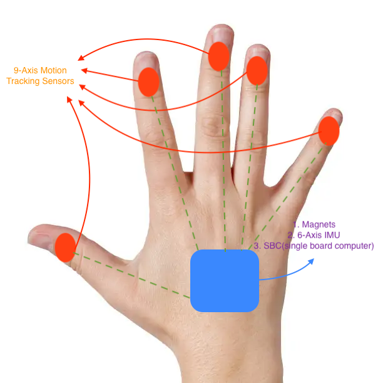
\includegraphics[width=.4\linewidth]{hardware/overall-hardware-structure.png}
    \caption{\label{fig:overall-hardware-structure}Overall Hardware Structure}
\end{figure}

为了使以上叙述更加清晰明了,以下列出并描述了位于手部的各硬件组件:
\begin{enumerate}
\item 每个指尖上都有一个9轴运动传感器
\item 手背上有一个磁铁(产生用于计算手指相对位置的磁场)
\item 手背上有一个6轴惯性传感器(IMU)
\item 手背上有一个单板计算机(Single Board Computer,SBC)(用于读取传感器数据并进行相应的计算)
\end{enumerate}

整个硬件系统的核心原则是在已知手指传感器与手背传感器相对姿态的情况下,使用磁偶极子模型估算指尖与手背的相对位置,如\autoref{fig:abstract-hardware-model}所示:

\begin{figure}[H]
    \centering
    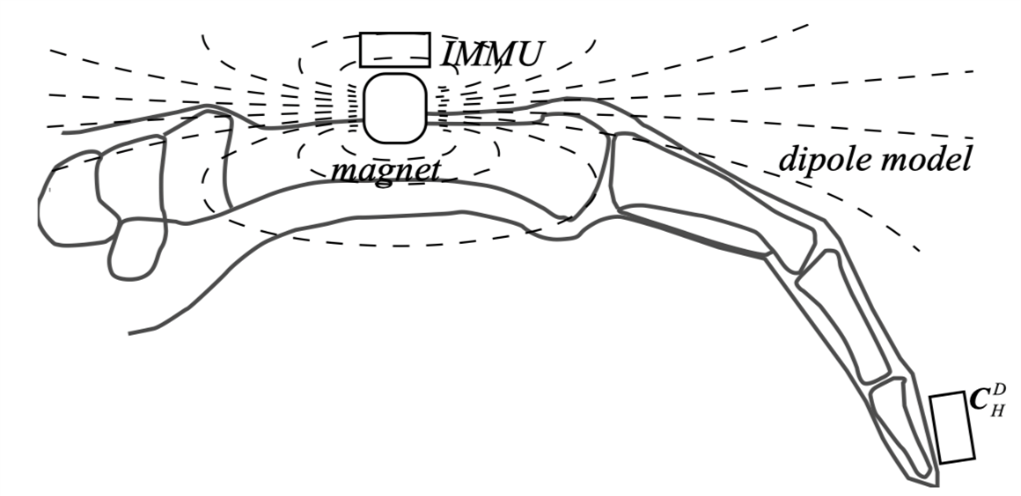
\includegraphics[width=.4\linewidth]{hardware/abstract-hardware-model.png}
    \caption{\label{fig:abstract-hardware-model}Abstract Hardware Model}
\end{figure}

针对多个传感器数据的采集,可以考虑使用I2C总线协议。\autoref{fig:connection-using-i2c-bus-protocol}展示了一种可行的传感器连接方式(\autoref{fig:connection-using-i2c-bus-protocol}中的传感器为ICM20948 9轴传感器)

\begin{figure}[H]
    \centering
    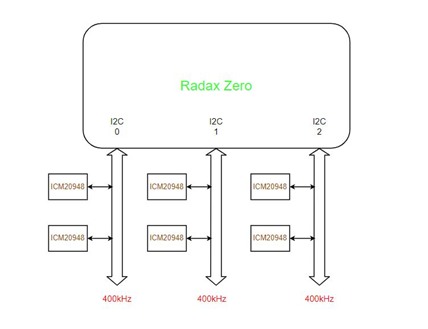
\includegraphics[width=.4\linewidth]{hardware/connection-using-i2c-bus-protocol.png}
    \caption{\label{fig:connection-using-i2c-bus-protocol}Connection Scheme Using I2C Bus Protocol}
\end{figure}

其中,每条I2C总线上连有两个相同的ICM20948传感器(I2C地址的最低位可以通过传感器上的某个特定管脚进行调整,故同一条I2C总线上最多可以容纳2个相同的传感器),总共需要3条I2C总线来对6个传感器进行数据读取。

\subsection{整体软件架构}

如\autoref{fig:connection-using-i2c-bus-protocol}所示,整个软件系统将运行在完整的Linux操作系统上。其中,{\bfseries \itshape enhanced\_icm20948}是自行开发的,包含有本毕业设计项目中很大一部分软件代码的开源库。其通过调用Eclipse基金会开发的{\bfseries \itshape mraa}开源通信库来实现对Linux开发板上I2C总线的访问与读取。

\begin{figure}[H]
    \centering
    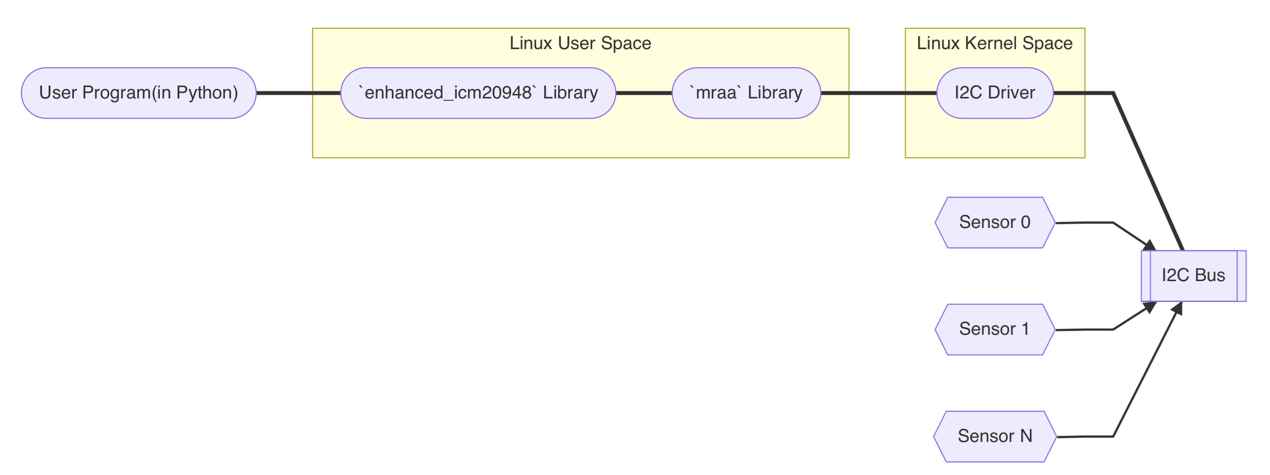
\includegraphics[width=0.85\linewidth]{software/overall-library-structure.png}
    \caption{\label{fig:overall-library-structure}Core Library Overall Structure}
\end{figure}

为了保证手指运动追踪系统计算的实时性与鲁棒性,整个开源库使用C++进行开发以实现最佳性能。如\autoref{fig:library-internal-structure}所示,{\bfseries \itshape enhanced\_icm20948}开源库主要包含3个模块,它们分别为:
\begin{enumerate}
    \item {\bfseries 传感器读取模块}: 负责高速读取各个传感器的数据
    \item {\bfseries 扩展卡尔曼滤波模块}: 负责计算手指端传感器与手背端传感器的相对姿态
    \item {\bfseries Python接口模块}: 通过使用{\bfseries \itshape Pybind11}来为由C++写成的高性能代码提供Python调用接口,以方便后续对数据的处理与深度学习技术的应用
\end{enumerate}

\begin{figure}[H]
    \centering
    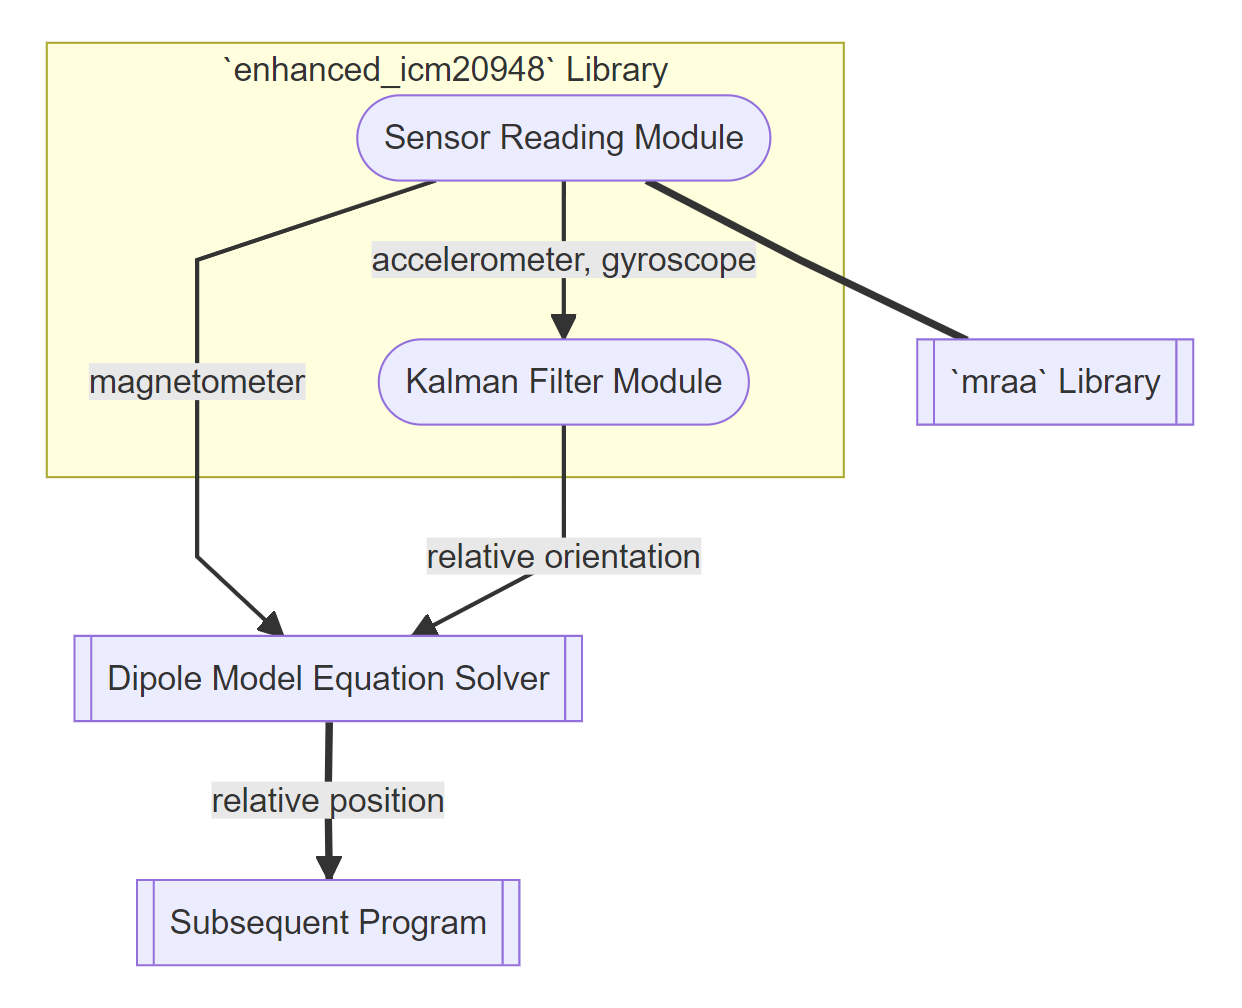
\includegraphics[width=0.4\linewidth]{software/library-internal-structure.png}
    \caption{\label{fig:library-internal-structure}Core Library Internal Structure}
\end{figure}

同时,由于整个开源库均使用标准C++并针对通用Linux内核进行开发,其可以在几乎所有的Linux发行版上正常工作运行。

本毕设项目中的后续应用及相应流程可以总结如下,如\autoref{fig:subsequent-program-structure}所示:
\begin{enumerate}
    \item 使用先前计算得到的相对位置进行动态手指追踪
    \item 使用深度学习技术进行实时手势识别
\end{enumerate}

\begin{figure}[H]
    \centering
    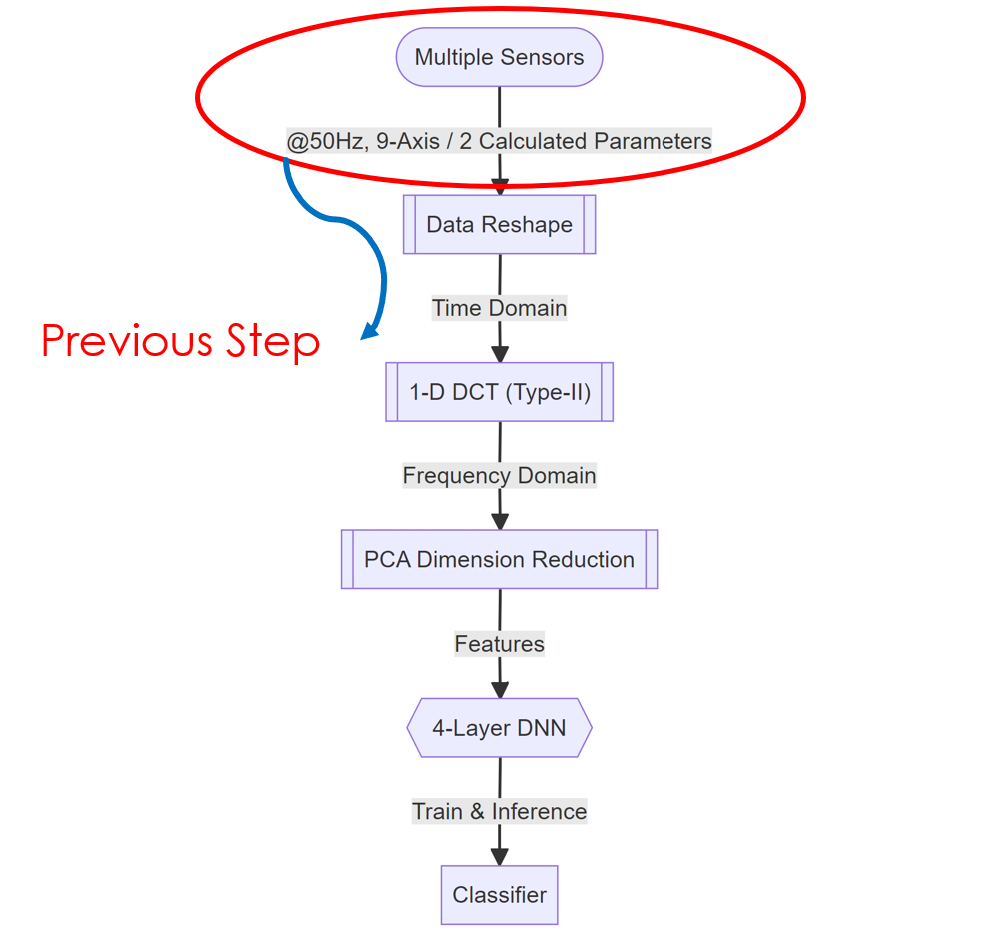
\includegraphics[width=0.4\linewidth]{software/subsequent-program-structure.png}
    \caption{\label{fig:subsequent-program-structure}Subsequent Dynamic Tracking and Gesture Recognition}
\end{figure}

\subsection{整体工作流程}
总体而言,如\autoref{fig:system-overall-workflow}所示,本毕设项目的整体系统按照以下工作流程运作:
\begin{enumerate}
    \item 首先,系统将使用扩展卡尔曼滤波(EKF),通过从各个传感器上采集到的加速度计与陀螺仪数据来计算各手指与手背之间的相对姿态
    \item 之后,系统将进一步使用磁偶极子模型与非线性方程组求解器,通过刚刚计算得到的相对姿态与传感器采集到的磁力计数据来解算各手指与手背之间的相对位置坐标
    \item 最后,计算得到的相对位置坐标将被进一步进行处理并应用深度学习技术以实现手指运动追踪与其它相应功能
\end{enumerate}

\begin{figure}[H]
    \centering
    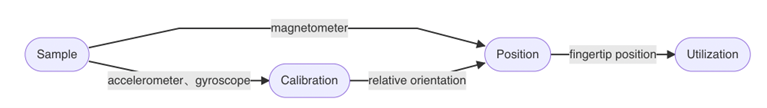
\includegraphics[width=\linewidth]{software/system-overall-workflow.png}
    \caption{\label{fig:system-overall-workflow}System Overall Workflow}
\end{figure}

值得注意的是,本毕设项目中自行开发并使用的核心开源库使用标准的C++进行编写,与多种Linux发行版兼容,使其具有高度的通用性和适应性。在接下来的几章中,本毕业设计项目的整个系统将被划分为4个部分,并进行独立的说明和讨论。

\cleardoublepage
\section{硬件系统设计与构建}
\subsection{硬件规格与参数}
本毕设项目使用了各种不同的硬件。将这些不同的硬件设备组合在一起,通过它们之间的相互配合实现特定的功能并完成此毕业设计项目中的任务,实现硬件协同。
此节将详细描述本毕设项目中所使用的各类硬件的具体参数及规格
\subsubsection{单板计算机}
本毕设项目中使用固定在手背上的单板计算机(Single Board Computer, SBC)作为核心计算设备。其不仅负责读取来自多个传感器的数据、计算手指传感器与手背传感器之间的相对姿态,同时也负责手指相对于手背位置的计算和自行训练的深度学习手势识别模型的实时推理。
为能够顺利完成上述的较为复杂的各类计算任务,同时也兼顾可维护性、可拓展性,我最终选取了树莓派4B作为此次毕设项目中的核心计算部件。\autoref{tab:raspberry-pi-spec}是树莓派4B的具体参数与规格:
\begin{table}[ht]
    \caption{\label{tab:raspberry-pi-spec}Raspberry Pi 4B Hardware Spec}
    \begin{tabularx}{\linewidth}{|c|X<{\centering}|}
        \hline
        {\bfseries Model} & Raspberry Pi 4B \\ \hline
        {\bfseries RAM} & 2GB \\ \hline
        {\bfseries CPU} & Broadcom BCM2711, Quad-core Cortex-A72 (ARM v8) 64-bit SoC \\ \hline
        {\bfseries GPU} & VideoCore VI, supports OpenGL ES 3.x and 4Kp60 hardware decoding of H.265 (HEVC) video \\ \hline
        {\bfseries Ports} & 2 x USB 3.0 ports, 2 x USB 2.0 ports, 2 x micro HDMI ports (up to 4Kp60 supported) \\ \hline
        {\bfseries Storage} & 64GB MicroSD card\\ \hline
        {\bfseries GPIO} & 40-pin GPIO header, with 3 I2C buses enabled\\ \hline
        {\bfseries Operating System} & Raspberry Pi OS (32 bits) \\ \hline
    \end{tabularx}
\end{table}

其外形如\autoref{fig:raspberry-pi-4b-appearance}所示:

\begin{figure}[H]
    \centering
    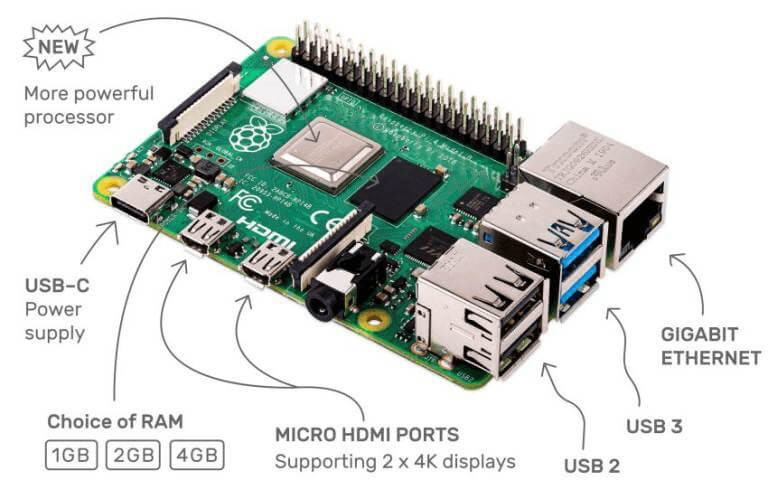
\includegraphics[width=.4\linewidth]{hardware/raspberry-pi-4b-appearance.png}
    \caption{\label{fig:raspberry-pi-4b-appearance}Raspberry Pi 4B Appearance}
\end{figure}

\subsubsection{传感器}
ICM20948是一款高度集成的惯性测量单元(IMU),具有三轴加速度计、三轴陀螺仪和三轴磁力计的功能。本次毕设项目中的全部6个传感器都选择了ICM20948。其通常被认为是MPU9250的升级版(MPU9250现已停产),具有更优秀的性能,能够很好的满足本毕业设计项目中的各项需求。以下是ICM20948传感器的核心参数与规格:
\begin{enumerate}
    \item {\bfseries Accelerometer}:
        \begin{itemize}
            \item Measurement Range: ±2 g, ±4 g, ±8 g, ±16 g
            \item Resolution: Up to 16384 LSB/g
        \end{itemize}
    \item {\bfseries Gyroscope}:
        \begin{itemize}
            \item Measurement Range: ±250 °/s, ±500 °/s, ±1000 °/s, ±2000 °/s
            \item Resolution: Up to 131 LSB/°/s
        \end{itemize}
    \item {\bfseries Magnetometer}:
        \begin{itemize}
            \item Measurement Range: ±4900 μT
            \item Resolution: Up to 0.15 μT
        \end{itemize}
    \item {\bfseries Communication}:
        \begin{itemize}
            \item I2C Bus: Supports data transfer rates up to 400 kHz
            \item SPI Bus: Supports data transfer rates up to 8 MHz
        \end{itemize}
\end{enumerate}


\subsection{PCB设计与布局}
在本毕设项目一开始的测试与验证阶段,面包板与杜邦线被直接用于拓展I2C总线并连接相应的传感器,如\autoref{fig:mess-connection}所示。这样的连接有以下几个非常大的问题与缺陷:
\begin{itemize}
    \item {\bfseries 信号干扰}:杜邦线通常没有屏蔽层,容易受到外部电磁干扰的影响,导致传感器信号的质量下降。这可能导致数据错误或不稳定性能
    \item {\bfseries 接触不可靠}:杜邦线的接触可靠性可能不高,容易出现接触不良或松动的情况。这可能导致传感器数据的不稳定性或中断
    \item {\bfseries 信号串扰}:当使用多条杜邦线在面包板上连接多个传感器时,信号可能会相互干扰,造成数据交叉或失真
    \item {\bfseries 硬件不稳定性}:面包板上的连接可能不够牢固,容易发生杜邦线松动或脱落的情况,导致系统不稳定或失效
\end{itemize}

\begin{figure}[H]
    \centering
    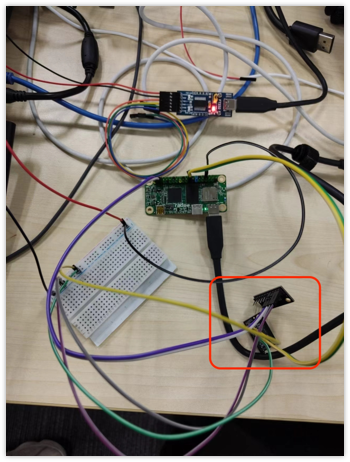
\includegraphics[width=.4\linewidth]{hardware/mess-connection.png}
    \caption{\label{fig:mess-connection}Initial Unstable Connection}
\end{figure}

为了解决这个问题,及能够通过I2C总线同时完成对6个传感器数据的高速读取并保证整体设备在进行各种运动时的连线稳定,我根据毕业设计的实际需求自行设计并打印了兼容树莓派4B 40Pins引脚的I2C总线扩展板。其电路原理图及布线图分别如\autoref{fig:pcb-schematic}和\autoref{fig:pcb-wiring}所示:

\begin{figure}[H]
    \centering
    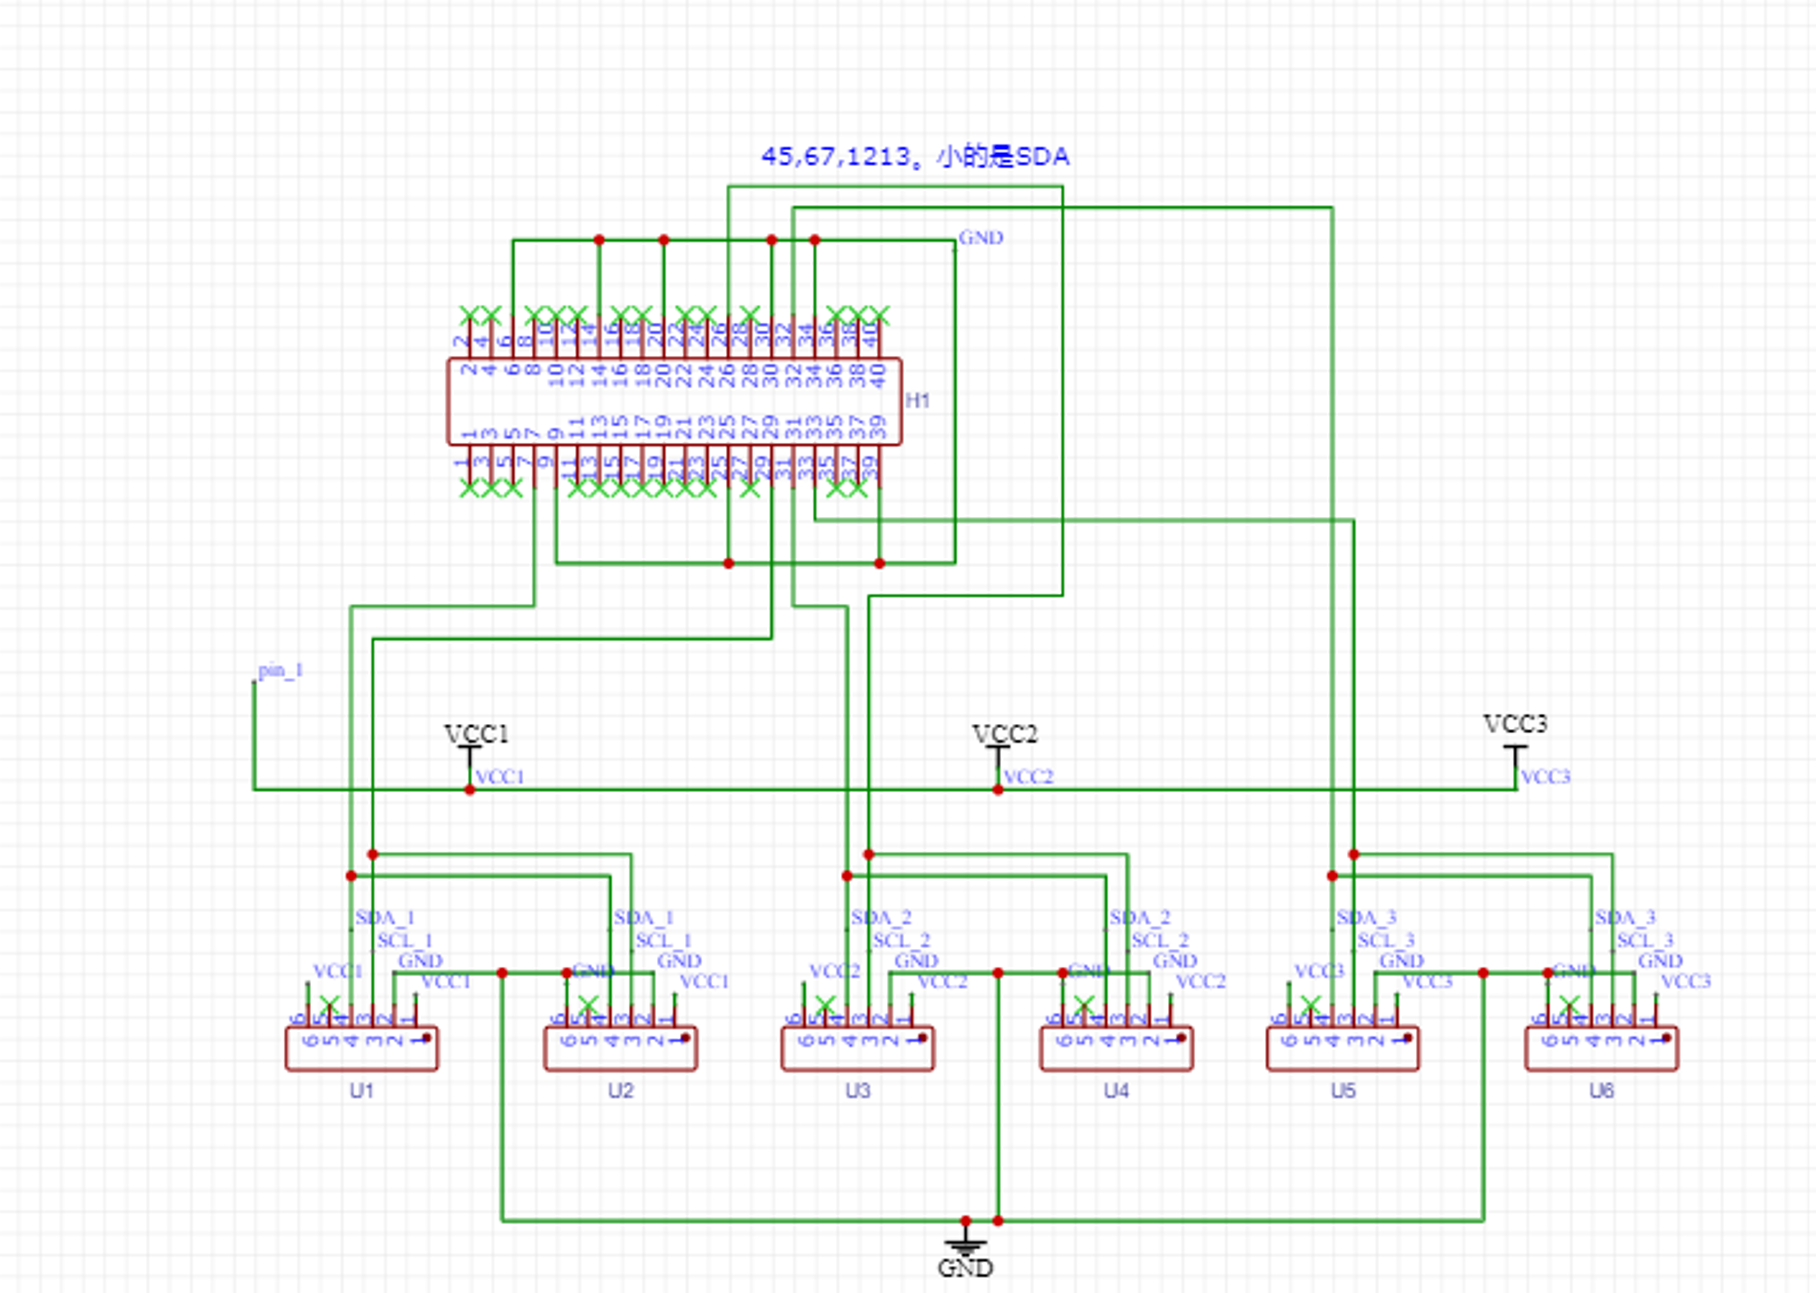
\includegraphics[width=.6\linewidth]{hardware/pcb-schematic.png}
    \caption{\label{fig:pcb-schematic}PCB Circuit Schematic}
\end{figure}

\begin{figure}[H]
    \centering
    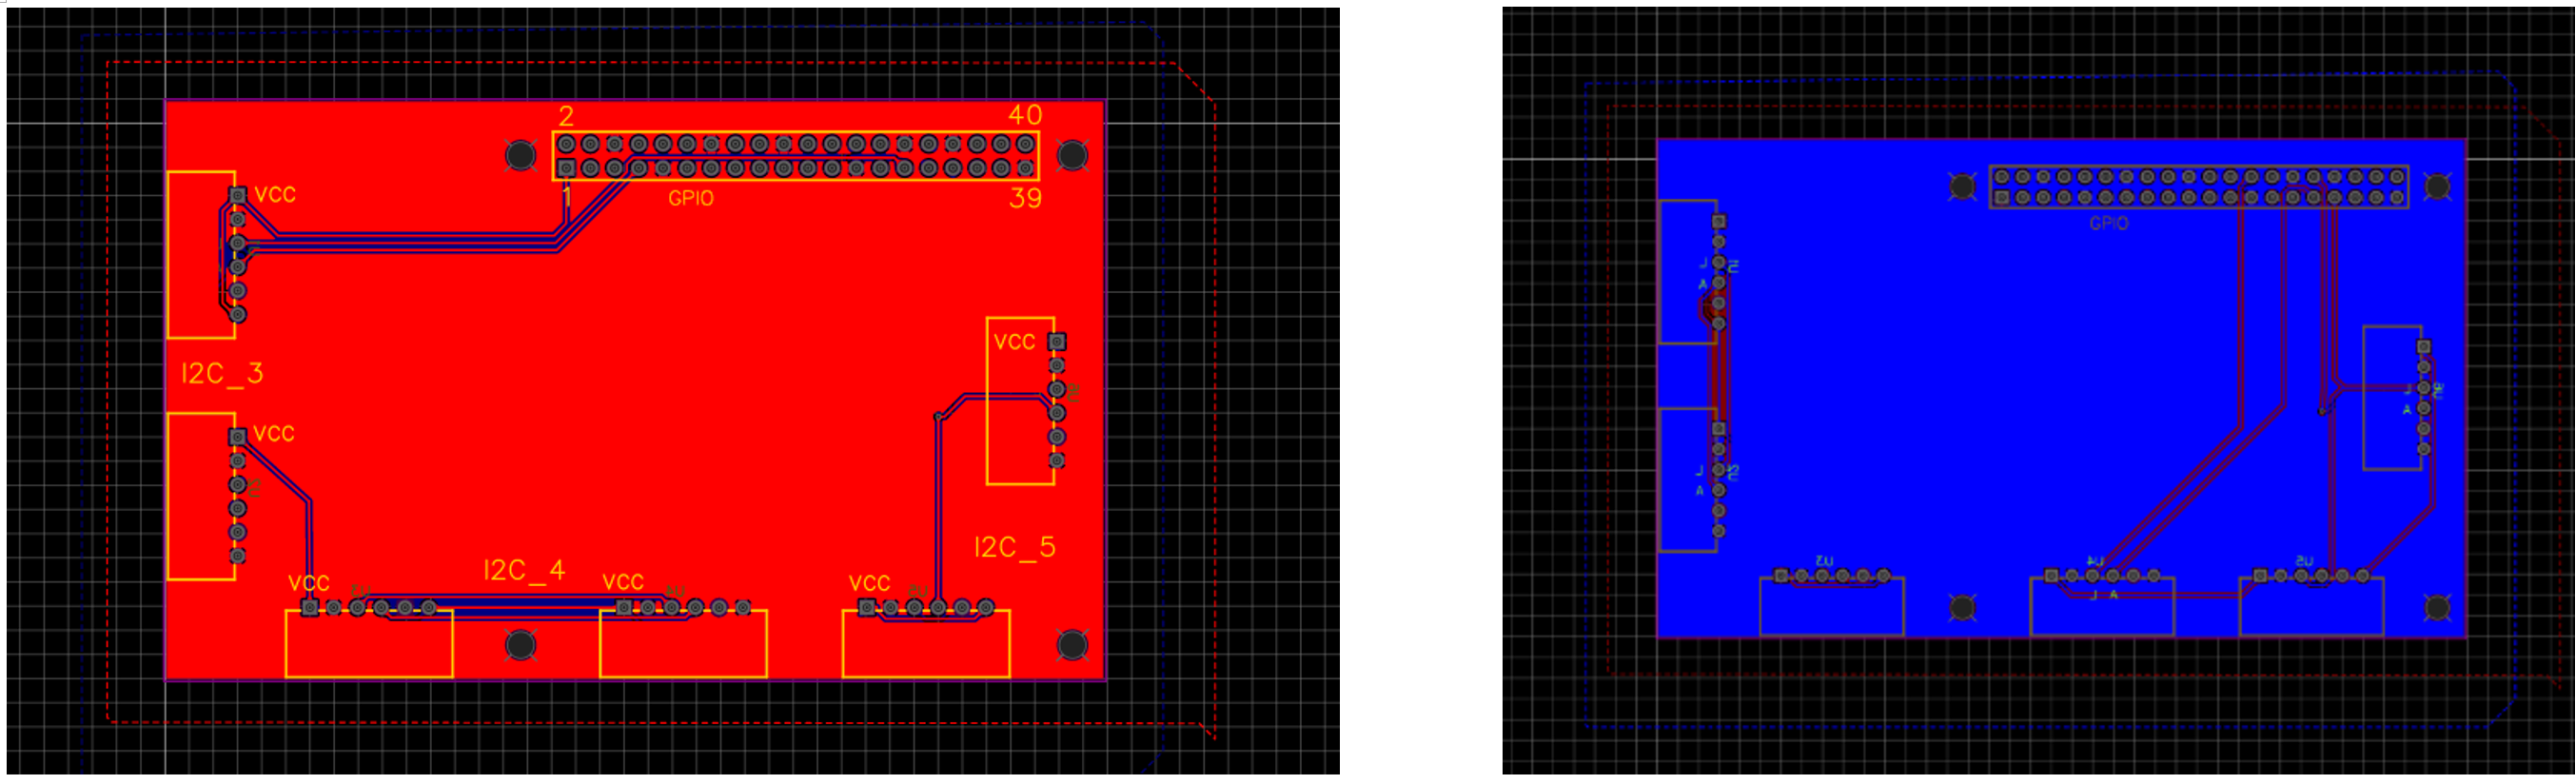
\includegraphics[width=\linewidth]{hardware/pcb-wiring.png}
    \caption{\label{fig:pcb-wiring}PCB Wiring Diagram}
\end{figure}

实物图如\autoref{fig:pcb-appearance}所示(能够与树莓派4B 40Pins引脚紧密插合)。其将树莓派4B上的3条I2C总线进行了扩展,使得每一条I2C总线上能够容纳2个传感器:

\begin{figure}[H]
    \centering
    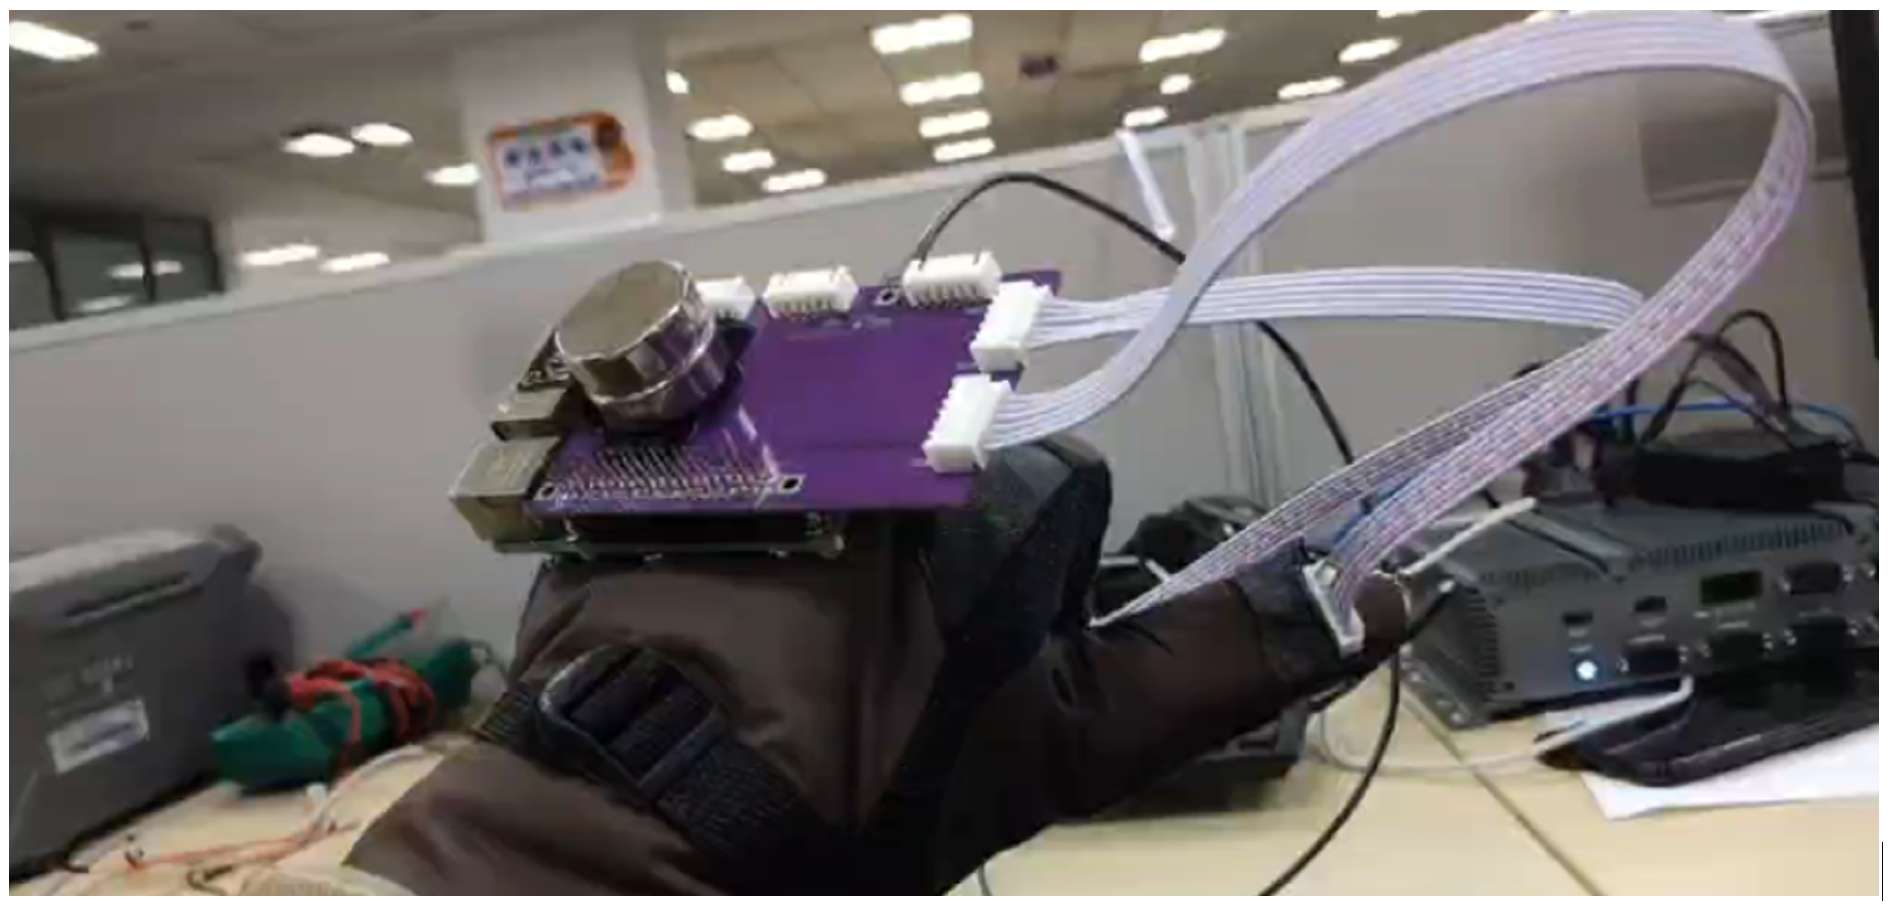
\includegraphics[width=.6\linewidth]{hardware/pcb-appearance.png}
    \caption{\label{fig:pcb-appearance}Designed and Printed PCB Board (Purple)}
\end{figure}

同时,得益于PCB设计,整体系统各个部件之间的连接稳定、可靠,为后续的动态手指追踪与实时手势识别提供了良好的硬件支持。
\subsection{硬件系统构建}
在本毕设项目中,一个绑定有一块永磁铁、6个传感器、1个单板计算机的手套被作为最终设备进行测试与开发,如\autoref{fig:entire-device-front}和\autoref{fig:entire-device-back}所示。
其中,圆柱形的永磁体作为磁场源被固定在位于手背的单板计算机上,为使用磁偶极子模型的定位算法提供磁场。
6个传感器中的5个分别位于手套的5个指尖,另一个同样被固定在位于手背的单板计算上,其紧邻永磁体,为定位算法提供相对位置的参考。
单板计算机与传感器通过上节中所提到的自行设计打印的PCB扩展板进行桥接,其连接稳定,能够在手指与手进行各种运动变换时正常工作。

\begin{figure}[H]
    \centering
    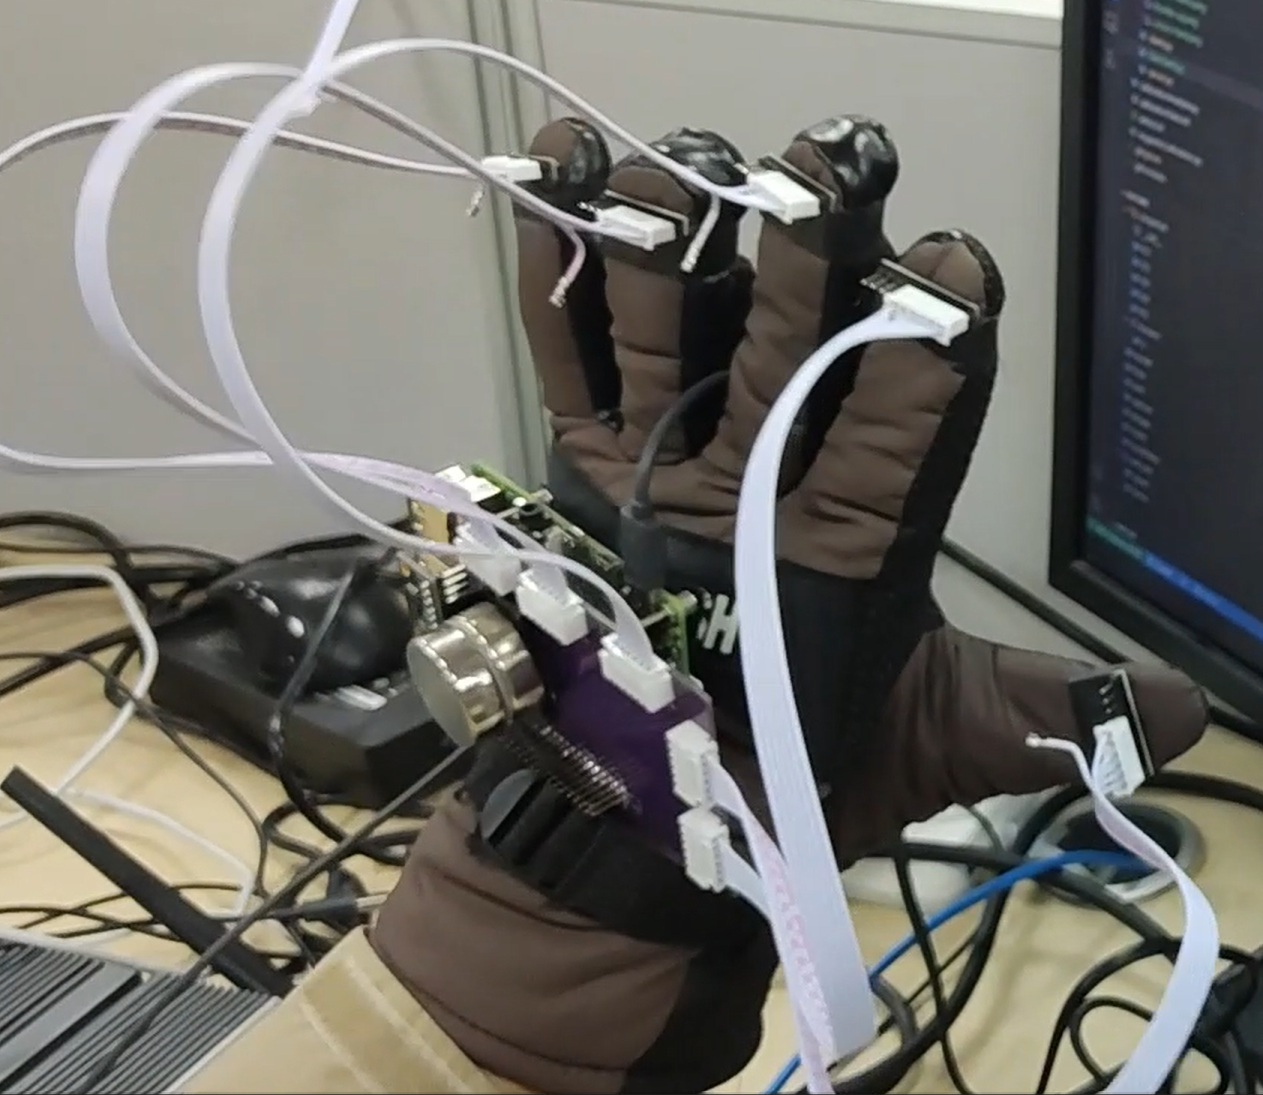
\includegraphics[width=.4\linewidth]{hardware/entire-device-front.png}
    \caption{\label{fig:entire-device-front}Final Device (Front View)}
\end{figure}

\begin{figure}[H]
    \centering
    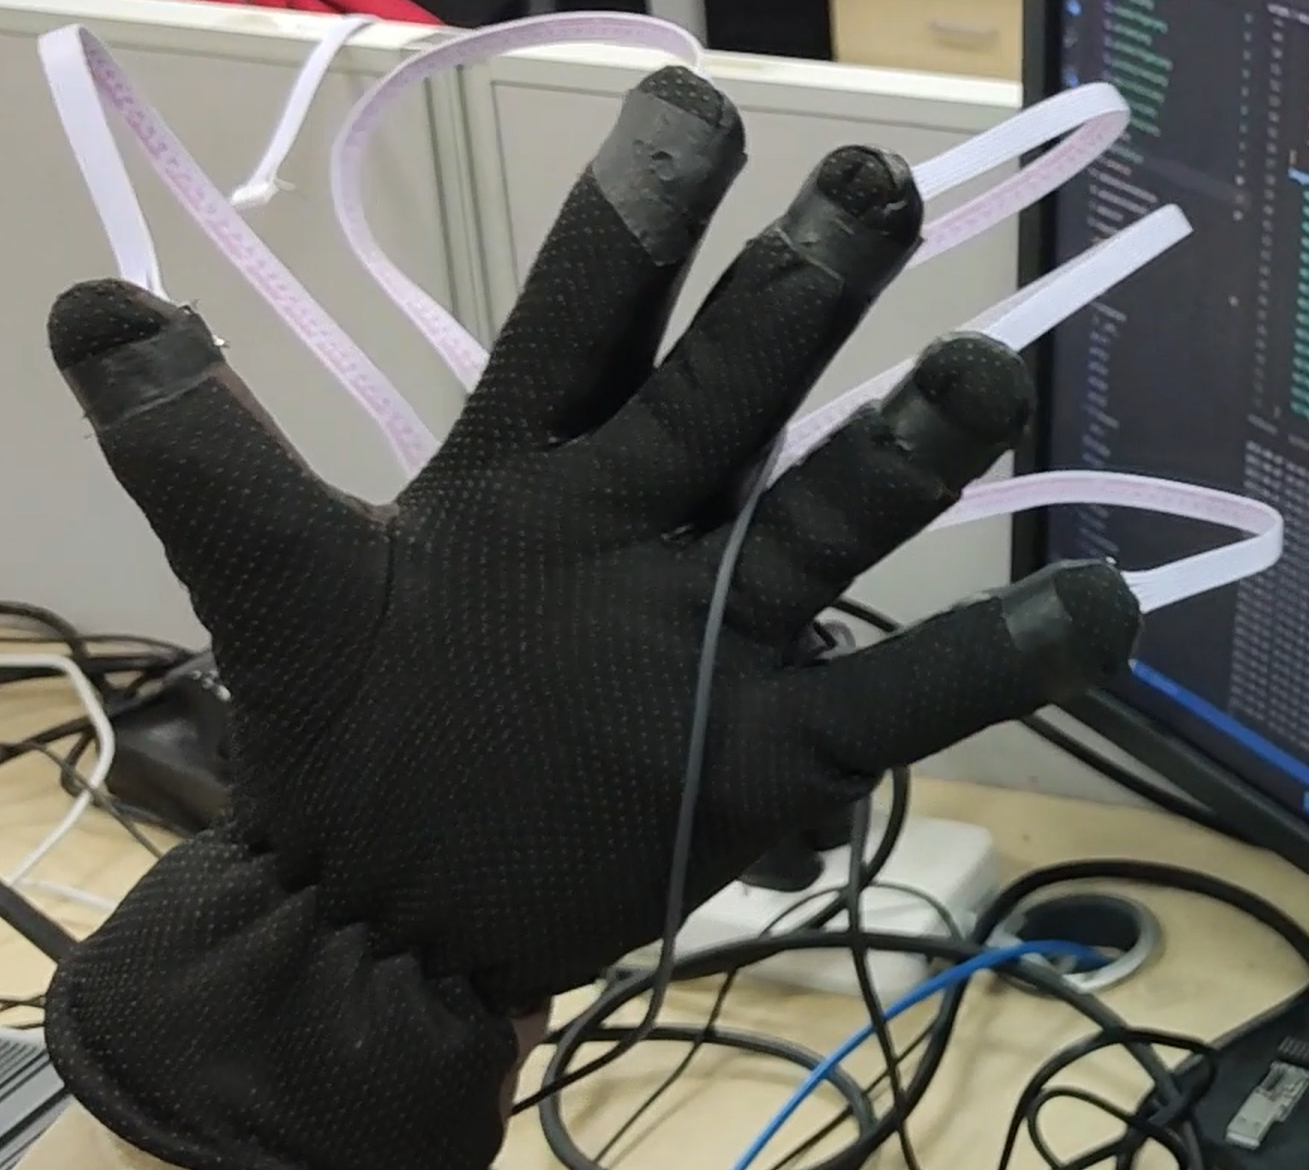
\includegraphics[width=.4\linewidth]{hardware/entire-device-back.png}
    \caption{\label{fig:entire-device-back}Final Device (Back View)}
\end{figure}

\cleardoublepage
\section{核心开源库}
\subsection{整体介绍}
{\bfseries 此库的所有代码均由本人编写并已发布在Python社区的官方软件包仓库上:\href{https://pypi.org/project/enhanced-icm20948/}{enhanced-icm20948}}

基于{\textbf \itshape libmraa},此自行开发的核心开源库,{\textbf \itshape enhanced\_icm20948},旨在为通用Linux开发板提供从ICM-20948 9轴运动传感器高速读取数据的工具(加速度计和陀螺仪的读取频率大于200Hz,磁力计的读取频率大于100Hz)。

该库的核心代码由C++编写,并借助{\bfseries \itshape Pybind11}提供基于Python的API接口。该库还支持同时从多个I2C总线上的多个ICM-20948传感器读取数据。此外,只要没有地址冲突,它还支持在单个I2C总线上读取多个传感器的数据。然而,在这种情况下,由于I2C总线通信频率的限制,读取数据的速度可能会受到限制。

除此之外,该库还基于{\bfseries \itshape Eigen3}线性代数运算库实现了扩展卡尔曼滤波(EKF)算法,并具有相当高的效率,能够支持不同传感器之间的实时相对姿态估计。

\subsection{高性能实现}
\subsubsection{C++后端}
通常,对各类传感器数据的读取与处理会交由嵌入式开发板来完成。嵌入式开发板的型号数量非常庞大,而且种类各异。各个厂商和供应商提供了许多不同类型的嵌入式开发板,以满足不同应用和需求。这些开发板可能基于不同的处理器架构,如ARM、x86、MIPS等,具有不同的处理能力和功能集。它们还可能针对特定的应用领域进行优化,如物联网(IoT)、工业自动化、医疗设备、智能家居等。

一些常见的嵌入式开发板型号包括:Raspberry Pi系列,Arduino系列,BeagleBone系列,NVIDIA Jetson系列等。但是,相对于通用计算机或服务器,嵌入式开发板的性能通常十分有限。这是因为嵌入式系统的设计目标通常是在特定的应用场景中实现低功耗、高效能和紧凑的解决方案,如进行各类传感器数据的采集与处理。

为了实现在此类设备上对多种传感器进行实时、高速地数据读取与数据处理,最大限度利用硬件资源,C/C++往往会成为编写各类性能敏感程序的最佳选择。

在为本次毕业设计项目而开发的核心库中,所有的核心控制逻辑与计算过程均由C++实现,包括但不限于对传感器、I2C总线的访问读取逻辑,卡尔曼滤波算法的实现,工作线程池的创建与管理等。此外,得益于C++对硬件和系统资源的控制能力,多线程编程模型也在开发之初就被纳入了考虑并被广泛使用以最大限度利用系统资源,进一步提升性能与效率。

具体的实现细节与性能测试将会在本章中的之后几节详述
\subsubsection{多线程编程模型设计与管理}
多线程编程模型是一种充分利用现代多核心CPU,以充分发挥CPU的计算能力和并行处理能力的方法。通过将任务分解为多个独立的线程,并在多个处理器核心上同时执行这些线程,可以实现更高的吞吐量和更快的响应时间,如\autoref{fig:multithreading-benefits}所示。

\begin{figure}[H]
    \centering
    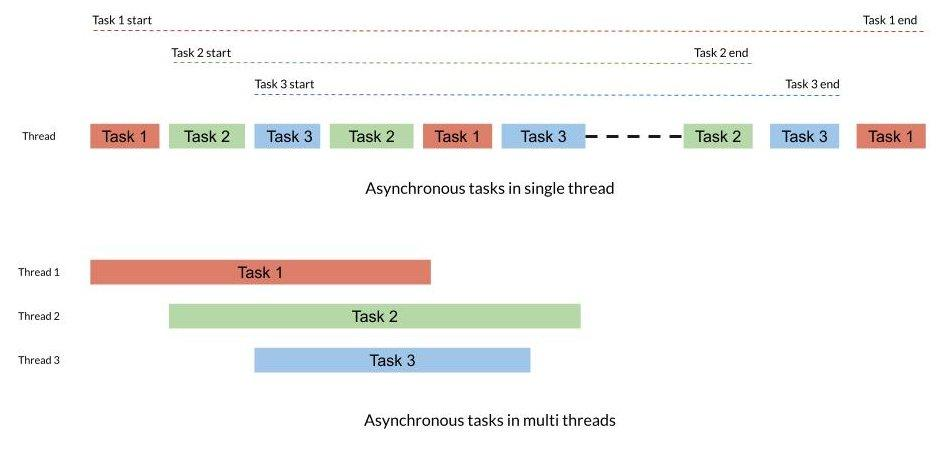
\includegraphics[width=0.7\linewidth]{library/multithreading-benefits.png}
    \caption{\label{fig:multithreading-benefits}Multithreading Benefits}
\end{figure}

在本毕业设计项目中,为了实现同时对多个传感器的高速数据读取与处理,多线程编程及线程池技术被充分应用,从而极大地提高了系统的整体性能与吞吐量,使之能够满足后续的动态传感器追踪与手势识别对数据处理速率的需求。

部分实现细节如\autoref{fig:multithreading-implementation-details}所示,其中,每个Reading Thread与1条物理I2C总线绑定,每条物理I2C总线上连接有两个物理传感器,其数据会被相应的Reading Thread读取并放置于内存中的Sensor Data Buffer。随后,Calculating Thread会从Sensor Data Buffer中读取所需的数据并使用卡尔曼滤波算法计算出各个传感器的相对姿态。最后,计算得到的传感器相对姿态会被放置于内存中的Orientation Data Buffer。

\begin{figure}[H]
    \centering
    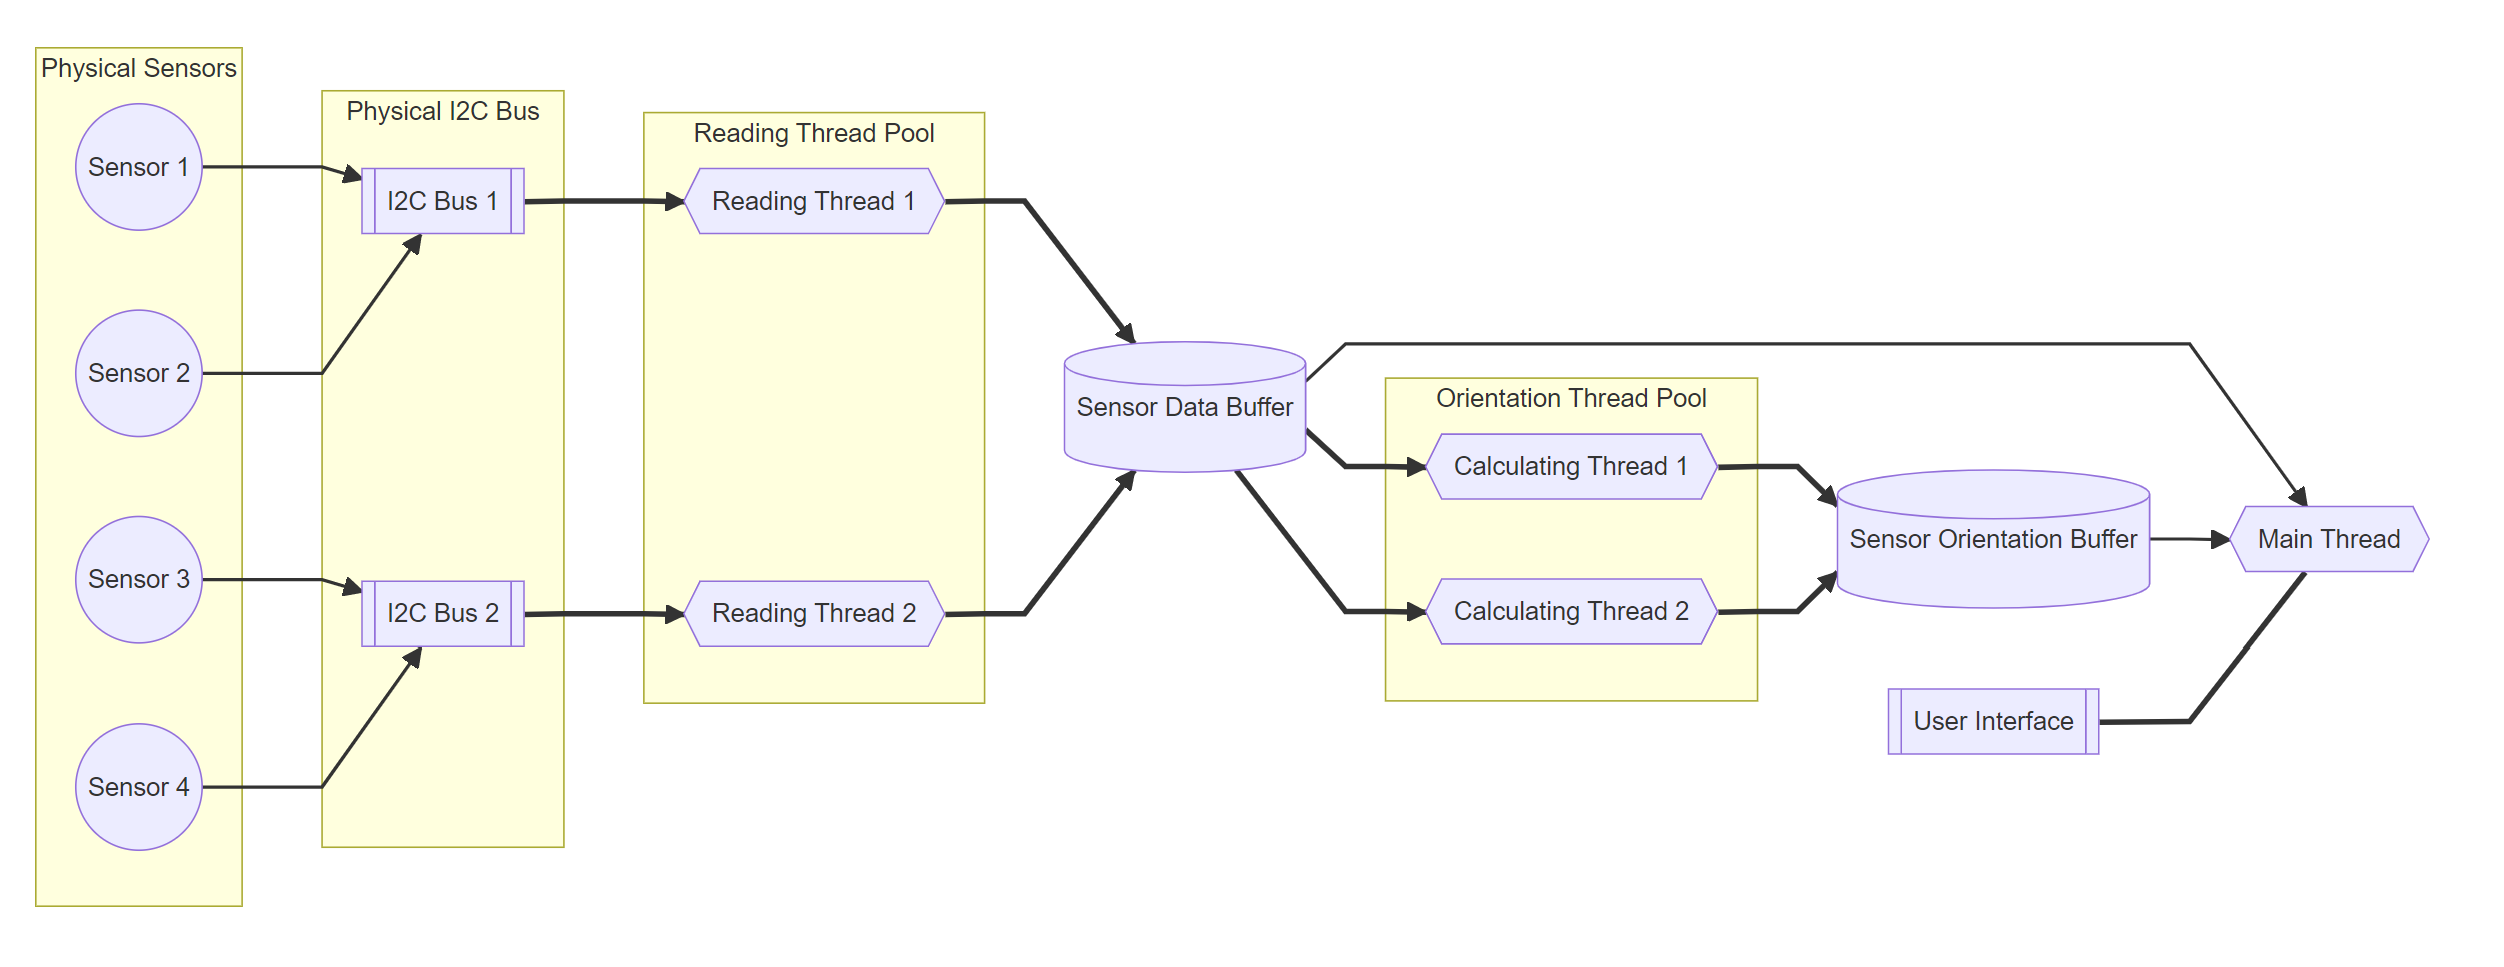
\includegraphics[width=\linewidth]{library/multithreading-implementation-details.png}
    \caption{\label{fig:multithreading-implementation-details}Multithreading Implementation Details}
\end{figure}

主线程负责管理Reading Thread Pool及Calculating Thread Pool中thread的创建与销毁,并提供相应的API以供调用此库的程序读取所需的数据、间接管理相关的工作线程以及设置相关的行为参数(包括但不限于:各传感器读取速率、卡尔曼滤波参数等)。

\subsubsection{低资源消耗}
通过合理使用阻塞式I/O、多线程模型和线程池,此库对系统资源的消耗较低。在树莓派4B平台上,仅使用此库的情况下,同时对6个传感器进行高速数据采集(200Hz+)并使用卡尔曼滤波算法实时计算它们的相对姿态时的资源消耗情况如\autoref{fig:low-resource-consumption}所示:

从\autoref{fig:low-resource-consumption}中可见,在上述情况下,此库于树莓派4B上能够在仅需要很少的CPU(15.2\% of 400\%)与内存(0.4\% of 100\%)开销的前提下实现高速的数据读取与卡尔曼滤波计算。

\begin{figure}[H]
    \centering
    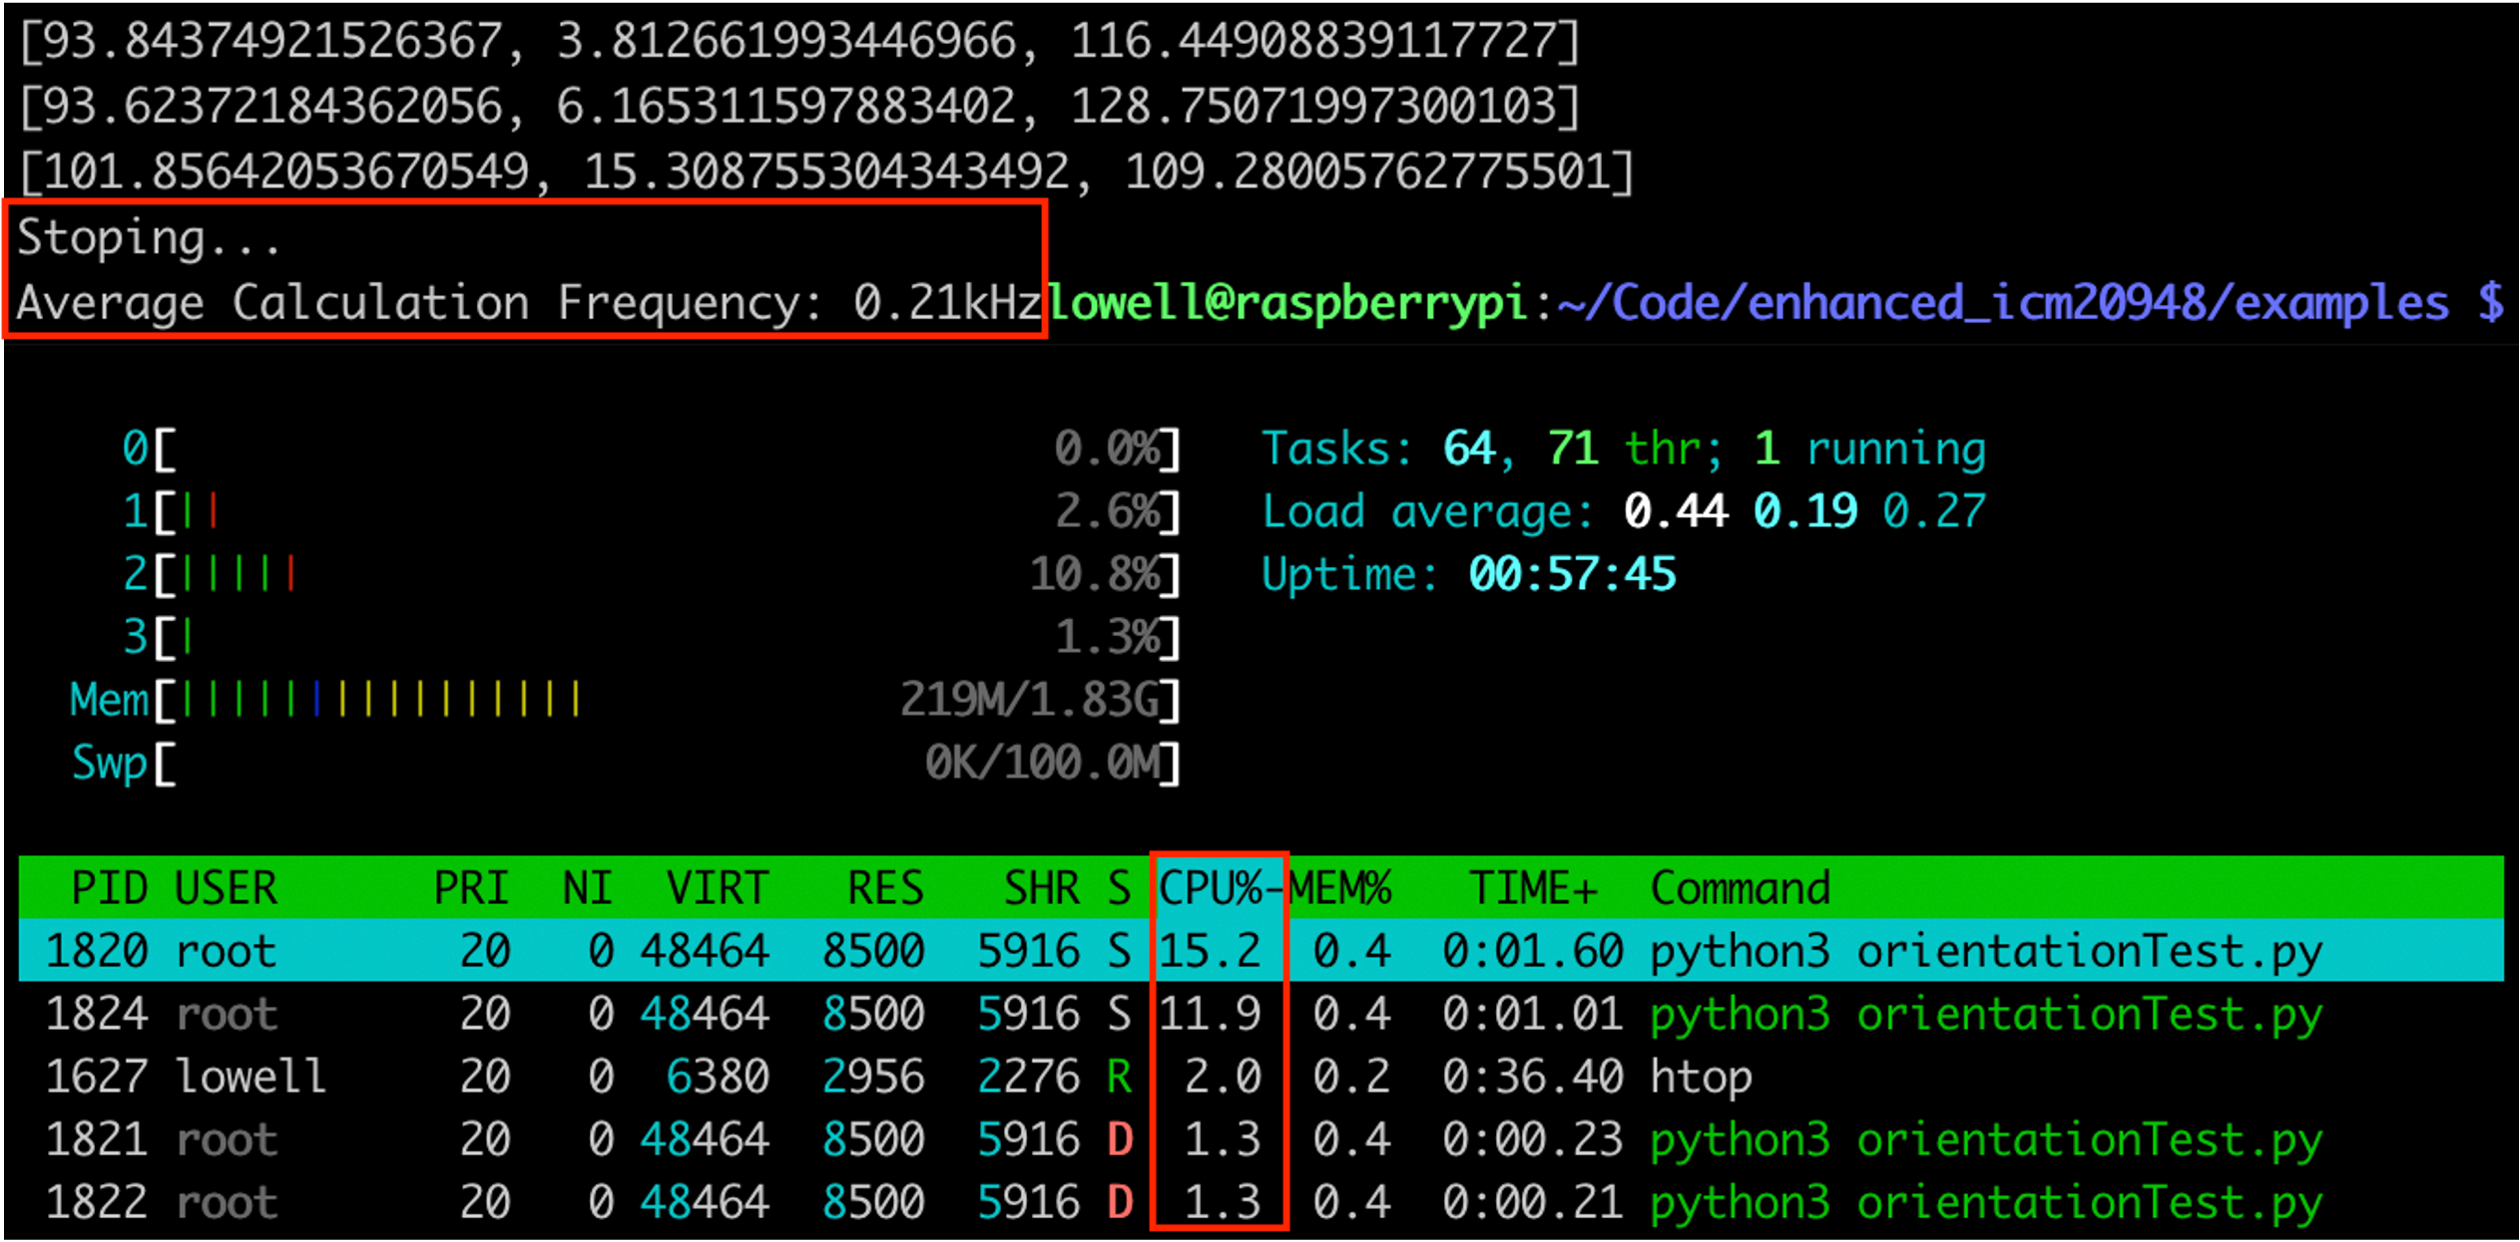
\includegraphics[width=0.6\linewidth]{library/low-resource-consumption.png}
    \caption{\label{fig:low-resource-consumption}Low Resource Consumption when Using the Library}
\end{figure}

\subsection{跨平台支持}
\subsubsection{Python Wrapper}
虽然C++的静态类型系统和直接内存访问使得它在计算密集型任务、底层系统开发和资源受限环境下具有性能和效率方面的优势。但在进行二次开发时,相比于Python,C++的开发效率相对而言非常低,因为其需要更多额外的工作来进行编码和调试,对于第三方用户的使用也非常不友好。
考虑到第三方用户的使用及整体系统后续的非线性方程组计算、实时数据处理与传输、深度学习模型训练与推理等一系列复杂流程,我使用{\bfseries \itshape Pybind11}开源工具库将已有的核心C++代码封装为Python模块,并将相关的API暴露给Python(如\autoref{fig:combine-python-and-c++}所示),从而可以在Python环境中直接调用和使用此库。
同时,这样做也可以充分发挥C++的高性能和Python的灵活性,大幅简化此毕设项目后续功能的开发、实现与验证。

\begin{figure}[H]
    \centering
    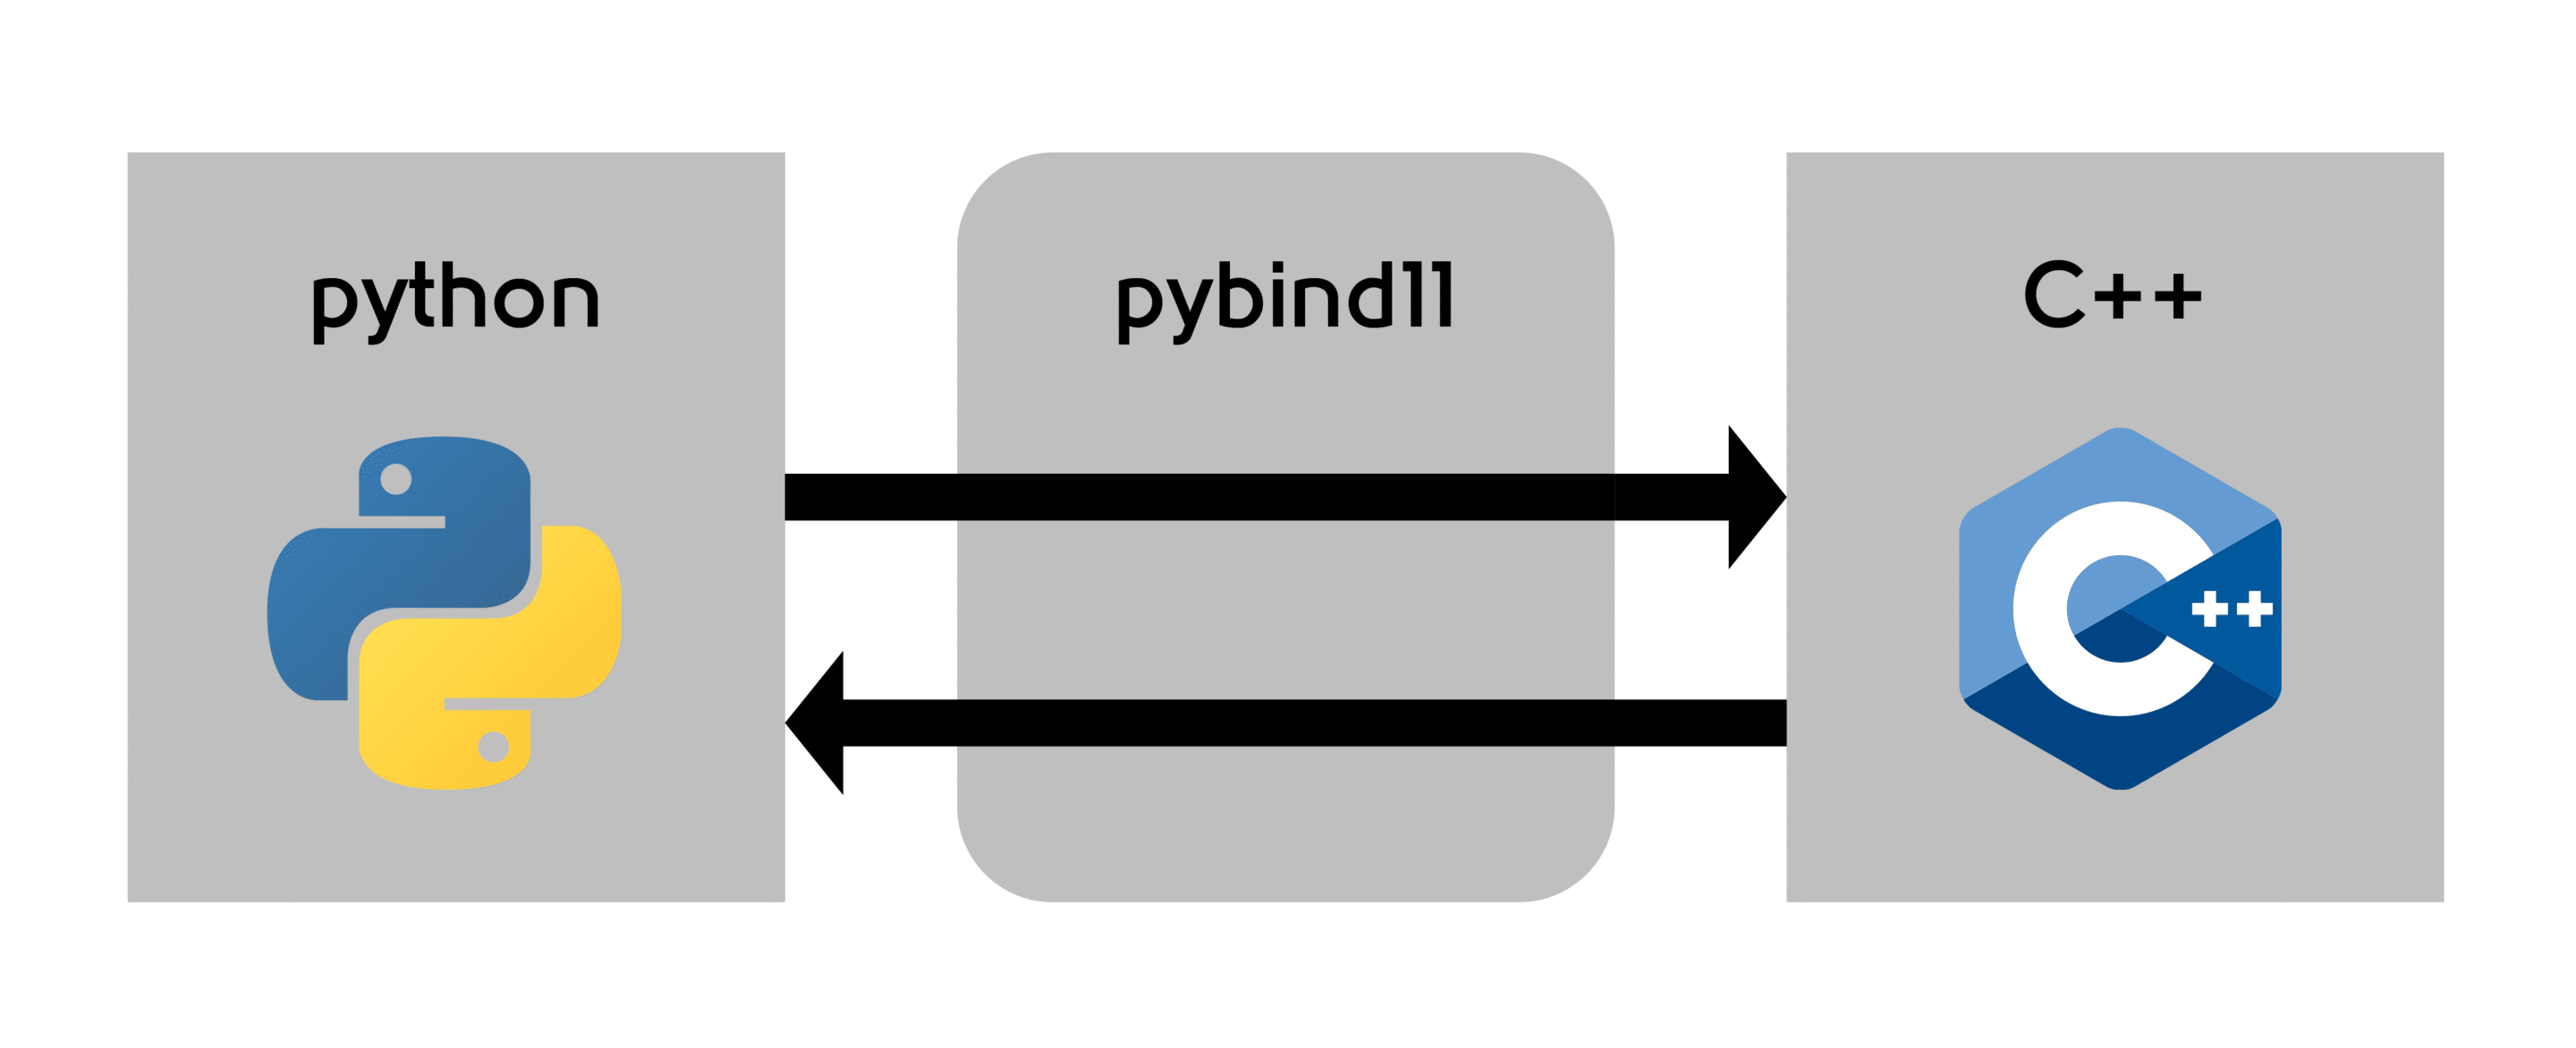
\includegraphics[width=0.5\linewidth]{library/combine-python-and-c++.png}
    \caption{\label{fig:combine-python-and-c++}Combine Python and C++ using Pybind11}
\end{figure}

\subsubsection{在PyPI上发布此库}
PyPI (Python Package Index) 是Python社区的官方软件包仓库。它是一个公共的、全球性的仓库,用于存储、发布和分发Python软件包。
开发者可以将自己编写的Python软件包上传到PyPI,以供其他用户下载和使用。用户可以使用命令行工具如pip或在开发环境中直接使用PyPI,从PyPI下载和安装软件包,以便在自己的项目中使用。

为了方便其它有需要的人的后续使用与研究,我已将此开源库打包(使用Setuptools)并上传至PyPI官方软件包仓库:\href{https://pypi.org/project/enhanced-icm20948/}{enhanced-icm20948},并撰写了相关的文档和使用说明。
任何人都可以使用pip命令行工具安装此库并进行使用与测试,如\autoref{fig:published-on-pypi}和\autoref{fig:install-the-library-using-pip}所示:

\begin{figure}[H]
    \centering
    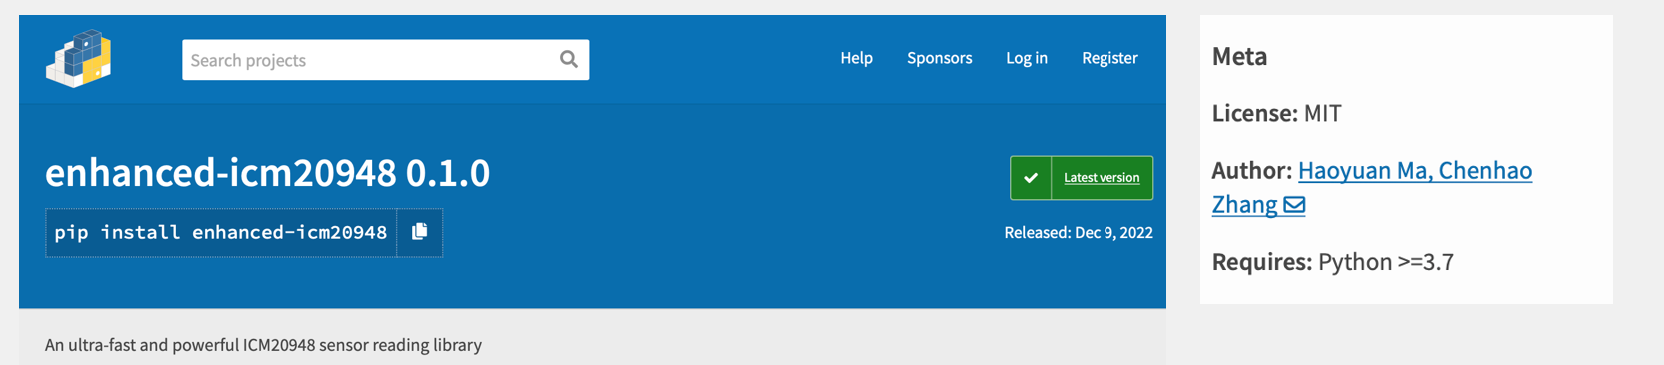
\includegraphics[width=0.75\linewidth]{library/published-on-pypi.png}
    \caption{\label{fig:published-on-pypi}The Library Published On PyPI}
\end{figure}

\begin{figure}[H]
    \centering
    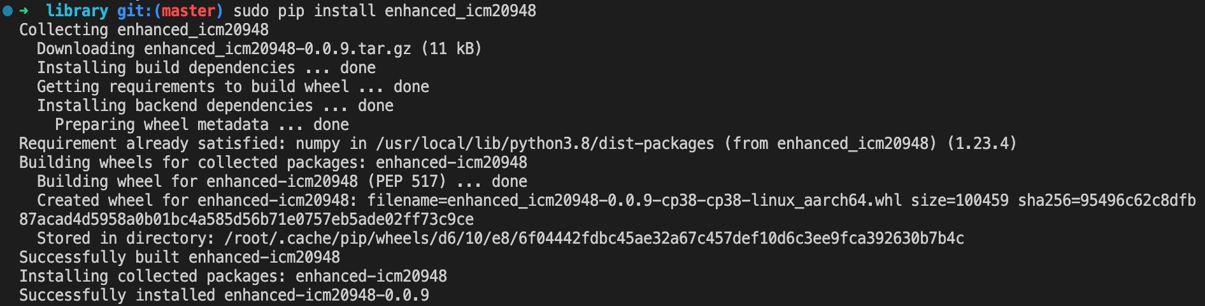
\includegraphics[width=0.75\linewidth]{library/install-the-library-using-pip.png}
    \caption{\label{fig:install-the-library-using-pip}Install the Library Using pip}
\end{figure}

\subsubsection{安装与测试手册}
以下是供参考的安装此库的说明:

\begin{enumerate}
    \item {\bfseries 安装相关依赖} \\
对于基于Ubuntu的系统,可以使用以下命令安装依赖项:
\begin{lstlisting}[%
    language={Bash},
    caption={Install Dependencies},
    label={code:install-dependencies}
]
sudo apt update
sudo apt install git build-essential swig3.0 libnode-dev \ 
cmake libjson-c-dev python3-pip python3-dev
\end{lstlisting}
    \item {\bfseries 安装libmraa} \\
如果当前使用的开发板已经有官方支持的libmraa,则强烈建议您通过相应的软件包管理器或开发板制造商提供的教程安装libmraa。
如果没有官方支持,则可以使用以下命令编译并安装libmraa:
\begin{lstlisting}[%
    language={Bash},
    caption={Install libmraa},
    label={code:install-libmraa}
]
# Clone libmraa gir repo
git clone https://github.com/eclipse/mraa.git
cd mraa
mkdir build
cd build
#########################################
###### if you use ARM-based boards ######
cmake .. -DBUILDSWIGPYTHON=OFF -DCMAKE_INSTALL_PREFIX:PATH=/usr \ 
-DBUILDARCH=arm
###### if you use X86-based boards ######
cmake .. -DBUILDSWIGPYTHON=OFF -DCMAKE_INSTALL_PREFIX:PATH=/usr
#########################################
# Build libmraa
make -j
# Install libmraa
sudo make install
# Update shared library cache
sudo ldconfig
\end{lstlisting}
    \item {\bfseries 安装enhanced-icm20948} \\
\begin{lstlisting}[%
    language={Bash},
    caption={Install enhanced-icm20948},
    label={code:install-enhanced-icm20948}
]
python3 -m pip install enhanced-icm20948
\end{lstlisting}
\end{enumerate}

\subsubsection{支持且经过测试的平台}
目前,此库所支持并通过安装测试的Linux发行版如\autoref{tab:library-platform}所示(包括但不限于):

\begin{table}[ht]
    \caption{\label{tab:library-platform}Supported and Tested Platform}
    \begin{tabularx}{\linewidth}{|c|X<{\centering}|}
        \hline
        {\bfseries Operating System} & {\bfseries Architecture} \\ \hline
        Ubuntu 22.04 & amd64, aarch64 \\ \hline
        Ubuntu 20.04 & amd64, aarch64 \\ \hline
        Raspberry Pi OS & aarch64, arm32 \\ \hline
        Debian 11 & aarch64, arm32 \\ \hline
    \end{tabularx}
\end{table}
请注意,此列表并非详尽无遗,该库可能也适用于其他Linux发行版。
\subsection{数据采集}
\subsubsection{并发数据读取}
此库支持通过多个I2C总线同时高速读取多个传感器的数据,其内部实现如\autoref{fig:sensor-reading-module-implementation}所示

\begin{figure}[H]
    \centering
    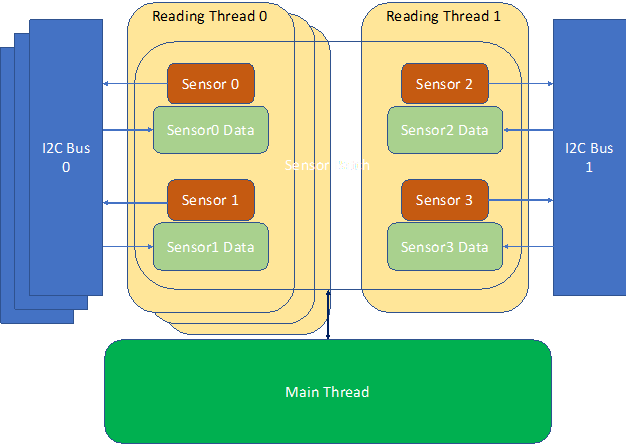
\includegraphics[width=0.5\linewidth]{library/sensor-reading-module-implementation.png}
    \caption{\label{fig:sensor-reading-module-implementation}Sensor Reading Module Implementation}
\end{figure}

如本章前几节所述,此库使用了多线程编程模型及线程池技术,以最大限度利用系统资源,提升系统的整体性能与吞吐量。线程锁、原子量等技术也根据需要被相应地使用,以对临界区进行有效保护,确保整体程序的正确性。
由于使用了{\bfseries \itshape Pybind11}对此库进行了Python封装,在实际Python环境中使用此库时,Reading Thread能够在后台自动地持续读取各传感器数据(通过相应API进行控制,之后几节会有介绍)。
此外,此数据读取模块在实现时采用了"Producer-Consumer Pattern"模式,Python程序作为"Consumer",能够通过相应的API读取库中暂存的传感器数据。

\subsubsection{I2C Bus Multiplexer}
在某些 Linux 开发板上,多条物理I2C总线外设可能在内部由多路复用器(Multiplexer)实现。多路复用器通常由硬件支持,并由相应的设备树(Device Tree)描述。设备树中的多路复用器节点描述了如何将多个 I2C 设备连接到同一物理 I2C 总线上,并通过选择不同的通道或地址进行访问。
对于此类开发板,在使用多个线程对多条I2C总线进行并发访问时,其正确性取决于开发板厂商所提供的设备驱动程序。在本次毕设项目进行的实验中,很多开发板厂商所提供的设备驱动程序无法正确处理多线程对I2C总线多路复用器的并发访问。
为此,此库针对此类情况提供了单线程多路复用数据读取功能。开启此功能时(通过相应的API,下一节会有介绍),只有一个Reading Thread会被创建,此Reading Thread会负责轮询各个I2C总线并读取连接在相应I2C总线上的传感器的数据。

\subsubsection{User Interface}
本节将会介绍此库中用于读取和控制传感器数据的部分重要API(Python Interface):
\begin{enumerate}
    \item {\bfseries 创建传感器并将其加入到SensorBatch} \\
可以使用如\autoref{code:create-sensor-and-sensor-batch}示例中的API创建传感器并将其加入到SensorBatch以便后续读取与管理
\begin{lstlisting}[%
    language={Python},
    caption={Create a sensor and add it to the SensorBatch},
    label={code:create-sensor-and-sensor-batch}
]
# Import library
from enhanced_icm20948 import sensors
# Create Sensors
firstSensor = sensors.ICM20948(i2cBus = 1, i2cAddress = 0x68, sensorName = "Hello")
secondSensor = sensors.ICM20948(i2cBus = 2, i2cAddress = 0x69, sensorName = "World")
# Create SensorBatch
sensorBatch = sensors.SensorBatch()
# Add Sensors to SensorBatch for later reading and management
sensorBatch.add_sensor(firstSensor)
sensorBatch.add_sensor(secondSensor)
\end{lstlisting}
    \item {\bfseries 启动数据读取} \\
如上一节所述,此库支持两种数据读取模式:多线程并发读取或单线程轮询读取。如\autoref{code:start-reading-thread}所示是两种读取方式的API:
\begin{lstlisting}[%
    language={Python},
    caption={Start reading thread},
    label={code:start-reading-thread}
]
# Import library
from enhanced_icm20948 import sensors
# Create Sensors
...
# Create SensorBatch
...
# Add Sensors to SensorBatch for later reading and management
...
# Start reading(multiple-thread version)
sensorBatch.start_reading()
# Start reading(single-thread version)
sensorBatch.start_sequential_reading()
\end{lstlisting}
    \item {\bfseries 读取库中暂存的数据} \\
可以使用如\autoref{code:retrieve-sensor-data}中所示的API来读取库中暂存的数据
Here are the APIs for retrieving sensor data from the library:
\begin{lstlisting}[%
    language={Python},
    caption={Retrieve sensor data},
    label={code:retrieve-sensor-data}
]
# Import library
from enhanced_icm20948 import sensors
# Create Sensors
firstSensor = sensors.ICM20948(i2cBus = 1, i2cAddress = 0x68, sensorName = "Hello")
# Create SensorBatch
...
# Add Sensors to SensorBatch for later reading and management
...
# Start reading
...
# Retrieving sensor data
# Get accelerometer data
accData = firstSensor.get_accel_data()
# Get gyroscope data
gyroData = firstSensor.get_gyro_data()
# Get magnetometer data
magData = firstSensor.get_mag_data()
\end{lstlisting}
    \item {\bfseries 停止数据读取} \\
可以使用如\autoref{code:stop-reading-thraed}中所示的API来停止数据读取:
The following APIs can be used to stop reading thread:
\begin{lstlisting}[%
    language={Python},
    caption={Stop reading thread},
    label={code:stop-reading-thraed}
]
# Import library
from enhanced_icm20948 import sensors
# Create Sensors
...
# Create SensorBatch
sensorBatch = sensors.SensorBatch()
# Add Sensors to SensorBatch for later reading and management
...
# Start reading
...
# Retrieving sensor data
...
# Stop reading thread
sensorBatch.stop_reading()
\end{lstlisting}
\end{enumerate}

\subsection{相对姿态计算}
\subsubsection{四元数简介}
四元数(Quaternion)是一种数学工具,用于表示旋转和方向。它扩展了传统的三维欧几里德空间中的复数概念,由一个实部和三个虚部组成,通常表示为$ q = a + bi + cj + dk$,其中$a,\ b,\ c,\ d$是实数,$i,\ j,\ k$是虚数单位。
在本毕业设计项目中,四元数主要被用于通过卡尔曼滤波算法来表示指尖传感器与手背传感器的相对姿态(坐标系三维旋转变化),如\autoref{fig:rotation-represented-by-quarternion}所示

\begin{figure}[H]
    \centering
    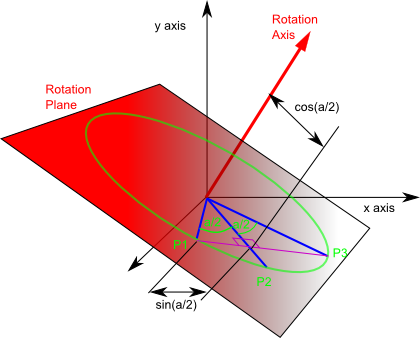
\includegraphics[width=0.5\linewidth]{library/rotation-represented-by-quarternion.png}
    \caption{\label{fig:rotation-represented-by-quarternion}Rotation Represented by Quarternion}
\end{figure}

\subsubsection{拓展卡尔曼滤波简介}
卡尔曼滤波(Kalman Filter)是一种基于状态空间模型的最优估计滤波器,用于通过测量值和系统模型来估计动态系统的状态。然而,许多实际应用中的系统模型都是非线性的,而卡尔曼滤波算法要求系统模型是线性的。这时,就需要使用扩展卡尔曼滤波来近似非线性系统模型,并在滤波过程中进行状态估计。

扩展卡尔曼滤波(Extended Kalman Filter,EKF)是一种卡尔曼滤波(Kalman Filter)的扩展版本,用于估计非线性系统的状态。与传统的卡尔曼滤波相比,EKF通过线性化非线性系统模型来处理非线性特性,从而能够更好地适应实际应用中的非线性问题。
EKF通过对非线性系统模型进行线性化,使用一阶泰勒展开来逼近非线性系统的状态转移函数和观测函数。然后,在每次更新步骤中,EKF使用线性化的模型来计算卡尔曼增益和估计误差协方差矩阵,进而进行状态估计和滤波更新,如\autoref{fig:extended-kalman-filter-step}所示。

\begin{figure}[H]
    \centering
    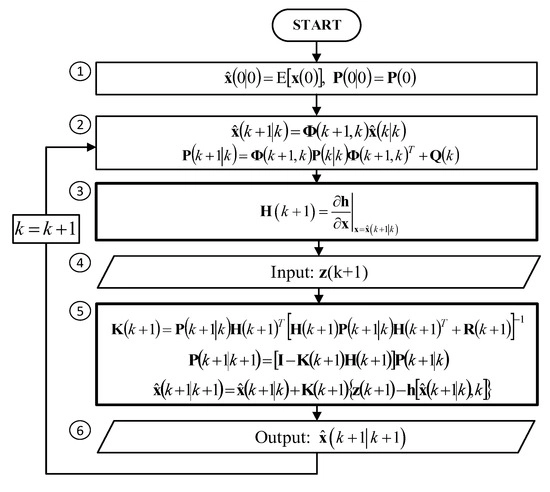
\includegraphics[width=0.5\linewidth]{library/extended-kalman-filter-step.png}
    \caption{\label{fig:extended-kalman-filter-step}Extended Kalman Filter Algorithm}
\end{figure}

扩展卡尔曼滤波(EKF)的基本步骤如下:
\begin{enumerate}
    \item {\bfseries 初始化}: 初始化状态估计值和误差协方差矩阵
    \item {\bfseries 预测步骤(状态预测)}: 根据线性化的状态转移函数,通过预测模型来估计下一个时刻的状态
    \item {\bfseries 更新步骤(状态更新)}: 根据线性化的观测函数,通过测量值来修正状态估计,并更新误差协方差矩阵
    \item {\bfseries 重复进行预测和更新步骤}: 不断迭代执行预测和更新步骤,以逐步更新状态估计和误差协方差矩阵,并逼近真实系统的状态
\end{enumerate}

\subsubsection{使用拓展卡尔曼滤波计算相对姿态}
在手部执行某些特定的动作和功能时,存在许多手和手指尖一起移动,经历几乎相同的角速度的情况。并且在这些特定情况下,不同传感器在其各自的三维坐标系中测量到的加速度几乎相同。
因此,我们假设在这些特定事件(designated events, DEs)期间和这些特定事件之间可以使用3D IMU充分估计手背与手指尖之间的相对姿态~\cite{mainArticle1}。

为了估计手指尖和手背之间的相对姿态,需要以一种最佳的方式将陀螺仪和加速度计的信息与特定事件(designated events, DEs)期间的额外信息进行融合。
因此,本毕业设计项目中引入了扩展卡尔曼滤波(EKF)算法来估计手指尖和手背之间的相对姿态(即假设手指尖和手背之间的角速度和加速度是相同的,只是在不同的坐标系下表示)。

扩展卡尔曼滤波(EKF)算法中的process model基于相对角速度的积分,measurement model主要基于DEs(特定事件)期间的信息。
DEs(特定事件)的质量被考虑在measurement variance中。
当DEs(特定事件)可用且方差较小时,我们更加相信measurement model;否则,我们更加相信process model。
因此,在手部执行某些特定的动作和功能时,此方法通过最佳融合process model和measurement model的信息来估计手指尖和手背之间的相对姿态~\cite{mainArticle1}。

\subsubsection{数学建模}
sensor model基于传感器增益误差和非正交误差具有时间不变性,且这些误差可以通过传感器校准获得的假设。
因此,经过校准的陀螺仪输出可以表示为\autoref{equ:outputs-of-gyroscope}:
\begin{equation}
    \label{equ:outputs-of-gyroscope}
    \begin{cases}
        y_{gyro,h}^h &= \omega_h^h + b_h + \zeta_h \\
        y_{gyro,f}^f &= \omega_f^f + b_f + \zeta_f
    \end{cases}
\end{equation}
其中,$y_{gyro,h}^h$和$y_{gyro,f}^f$分别是手背和指尖上的陀螺仪输出在它们各自的坐标系中的表示。
$b_x(x=h,f)$是缓慢变化的偏移量,$\zeta_x(x=h,f)$是高斯噪声。

对于校准后的加速度计,其在手背和指尖上的输出可以分别表示为\autoref{equ:outputs-of-accl}:
\begin{equation}
    \label{equ:outputs-of-accl}
    \begin{cases}
        y_{acc,h}^h &= a_h^h + g_h + \eta_h \\
        y_{acc,f}^f &= a_f^f + g_f + \eta_f
    \end{cases}
\end{equation}
其中,$g$代表重力加速度,$\eta_h$和$\eta_f$代表高斯噪声。

process model基于手背和手指尖之间在其各自坐标系中的相对角速度的积分。
我们选择表示手指尖到手背之间相对姿态的四元数$q_{hf} = [q_0\ \ q_1\ \ q_2\ \ q_3]^T$作为状态向量$x = q_{hf}$。相对姿态$x_k$的更新过程如\autoref{equ:process-model}所示:
\begin{equation}
    \label{equ:process-model}
    x_k = x_{k-1} \otimes [1\ \ \frac{1}{2}\omega_k d_t] + m
\end{equation}
其中,$m$是过程误差。$\omega_k$是手背和手指尖之间的相对角速度;$\otimes$表示两个四元数之间的乘法运算,如\autoref{equ:wk-definition}所示:
\begin{equation}
    \label{equ:wk-definition}
    \omega_k = (\omega_h^h)_k - x_{k-1} \otimes (\omega_f^f)_k \otimes x_{k-1}^{\star}
\end{equation}
其中,$\omega_h^h$和$\omega_f^f$分别表示手背和手指尖的角速度。

扩展卡尔曼滤波(EKF)的measurement model基于DEs(特定事件)。在DEs(特定事件)期间,手背和手指尖在不同的坐标系中共享相同的角速度,如\autoref{equ:de-share}所示:
\begin{equation}
    \label{equ:de-share}
    \omega_h^h = q_{hf} \otimes \omega_f^f \otimes q_{hf}^{\star}
\end{equation}
where $\omega_x^y(x=h,f;\ y=h,f)$ is the angular velocity of an object in frame $x$ expressed in the coordinate frame of object $y$. 
$h$ represents the hand and $f$ represents the finger tip.
其中,$\omega_x^y(x=h,f;\ y=h,f)$代表某个在坐标系$x$中的对象的角速度在$y$坐标系下的表示。
这里,$h$代表手背,$f$代表手指尖。

将\autoref{equ:outputs-of-gyroscope}和\autoref{equ:de-share}结合起来,我们可以得到\autoref{equ:shared-y-gyro-h-h}:
\begin{equation}
    \label{equ:shared-y-gyro-h-h}
    y_{gyro,h}^h = q_{hf} \otimes y_{gyro,f}^f \otimes q_{hf}^{\star} + d_{gyro}
\end{equation}

同样地,我们还可以得到\autoref{equ:shared-y-acc-h-h}:
\begin{equation}
    \label{equ:shared-y-acc-h-h}
    y_{acc,h}^h = q_{hf} \otimes y_{acc,f}^f \otimes q_{hf}^{\star} + (\lfloor w_h^h \rfloor_{\times} \lfloor w_h^h \rfloor_{\times} + \lfloor w_h^h \rfloor_{\times})r_{fh}^h  + \eta_c
\end{equation}

Subsequently, by combining \autoref{equ:shared-y-gyro-h-h} and \autoref{equ:shared-y-acc-h-h}, we can get the measurement model based on the sensor model and quaternion constraint:
接下来,通过结合\autoref{equ:shared-y-gyro-h-h}和\autoref{equ:shared-y-acc-h-h},我们可以得到基于sensor model和四元数约束的measurement model,如\autoref{equ:simplified-measurement-model}所示:
\begin{equation}
    \label{equ:simplified-measurement-model}
    y_k = f(x_k) + v
\end{equation}
其中,$y$和$f$可以表示为\autoref{equ:y-k}和\autoref{equ:measurement-model}:
\begin{equation}
    \label{equ:y-k}
    y_k = {[{(y_{acc,h}^h)}^T\ \ {(y_{gyro,h}^h)}^T\ \ 0]}^T
\end{equation}
\begin{equation}
    \label{equ:measurement-model}
    f(x) = \begin{bmatrix}
        x_k \otimes y_{acc,f}^f \otimes x_k^{\star} \\
        x_k \otimes y_{gyro,f}^f \otimes x_k^{\star} \\
        q_0^2 + q_1^2 + q_2^2 + q_3^2 - 1
    \end{bmatrix}
\end{equation}

如\autoref{equ:process-model}和\autoref{equ:measurement-model}所示,process model和measurement model都相对于$x_k$非线性。
为了更新$x_k$的协方差矩阵,需要进行线性化,并计算process model和measurement model的雅各比矩阵$F$和$H$。
详细过程及具体实现可以在此库的源代码中找到:\href{https://pypi.org/project/enhanced-icm20948/}{enhanced-icm20948}。
\subsubsection{并发计算}
此库支持同时计算多个传感器的相对姿态数据,其内部实现如\autoref{fig:kalman-module-implementation}所示

\begin{figure}[H]
    \centering
    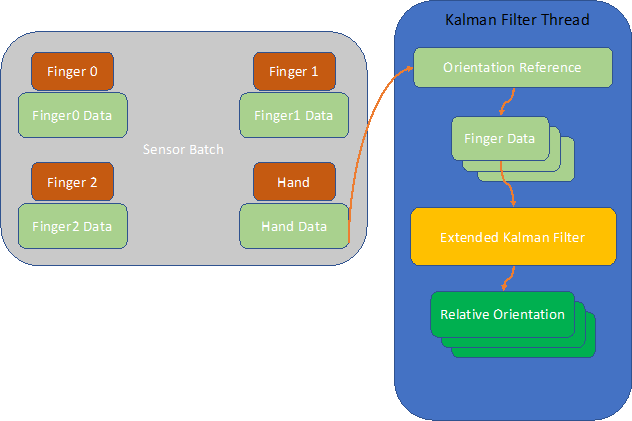
\includegraphics[width=0.5\linewidth]{library/kalman-module-implementation.png}
    \caption{\label{fig:kalman-module-implementation}Kalman Module Implementation}
\end{figure}

如本章前几节所述,此库使用了多线程编程模型及线程池技术,以最大限度利用系统资源,提升系统的整体性能与吞吐量。线程锁、原子量等技术也根据需要被相应地使用,以对临界区进行有效保护,确保整体程序的正确性。

由于使用了{\bfseries \itshape Pybind11}对此库进行了Python封装,在实际Python环境中使用此库时,Calculating Thread能够在后台自动地持续实时计算各传感器的相对姿态数据(通过相应API进行控制,之后几节会有介绍)。
此外,此卡尔曼滤波模块在实现时采用了"Producer-Consumer Pattern"模式,Python程序作为"Consumer",能够通过相应的API读取库中暂存的经过拓展卡尔曼滤波计算后得到的传感器相对姿态数据。

\subsubsection{实时性能}
由于扩展卡尔曼滤波涉及到大量的矩阵运算,为了加速计算过程,充分利用硬件资源,我在此库的开发过程中引入了第三方矩阵运算库Eigen。
Eigen是一个用于线性代数运算的C++模板库,提供了广泛的矩阵和向量操作功能。它采用了许多优化技术,包括表达式模板(expression templates)、编译时优化和向量化指令等,以提供高性能的线性代数计算。它在执行速度和内存使用方面表现出色,适用于大规模计算和实时计算。
此外,Eigen是一个纯头文件库,没有外部依赖,因此可以轻松地在各种操作系统和编译器上使用。它具有良好的跨平台支持,可以在多种硬件和软件环境中无缝运行。

得益于Eigen库的引入和使用,卡尔曼滤波算法能以相当高的效率执行。在树莓派4B平台上运行时,此库能以较低的延时和资源占用完成传感器之间相对姿态的实时计算与更新(200Hz+)

\subsubsection{用户接口}
本节将会介绍此库中用于读取和控制传感器相对姿态数据的部分重要API(Python Interface)
\begin{enumerate}
    \item {\bfseries 开始计算相对姿态} \\
可以使用如\autoref{code:start-calculating-thraed}中所示的API来开始计算指尖传感器与手背传感器的相对姿态:
\begin{lstlisting}[%
    language={Python},
    caption={Start calculating thread},
    label={code:start-calculating-thraed}
]
# Import library
from enhanced_icm20948 import sensors
# Create Sensors
...
# Create SensorBatch
sensorBatch = sensors.SensorBatch()
# Add Sensors to SensorBatch for later reading and management
...
# Start reading
...
# Start calculating orientation
sensors.start_estimating_orientation()
\end{lstlisting}
    \item {\bfseries 获取传感器相对姿态数据} \\
可以使用如\autoref{code:retrieve-orientation-data}中所示的API来获取传感器的相对姿态数据:
\begin{lstlisting}[%
    language={Python},
    caption={Retrieve orientation data},
    label={code:retrieve-orientation-data}
]
# Import library
from enhanced_icm20948 import sensors
# Create Sensors
firstSensor = sensors.ICM20948(i2cBus = 1, i2cAddress = 0x68, sensorName = "Hello")
# Create SensorBatch
...
# Add Sensors to SensorBatch for later reading and management
...
# Start reading
...
# Start calculating orientation
...
# Retrieve orientation data
firstSensor.get_orientation_quaternion()
\end{lstlisting}
    \item {\bfseries 停止传感器相对姿态计算} \\
可以使用如\autoref{code:stop-calculating-thread}中所示的API来停止对传感器相对姿态的计算:
\begin{lstlisting}[%
    language={Python},
    caption={Stop calculating thread},
    label={code:stop-calculating-thread}
]
# Import library
from enhanced_icm20948 import sensors
# Create Sensors
...
# Create SensorBatch
sensorBatch = sensors.SensorBatch()
# Add Sensors to SensorBatch for later reading and management
...
# Start reading
...
# Start calculating orientation
...
# Stop calculating orientation
sensorBatch.stop_estimating_orientation()
\end{lstlisting}
\end{enumerate}

\subsection{与现有解决方案的比较}
与现有的一些较为典型的第三方传感器数据读取库相比,此库在性能、效率、通用性等方面具有的优缺点如\autoref{tab:library-comparison}所示:
\begin{table}[ht]
    \caption{\label{tab:library-comparison}Library Comparison}
    \begin{tabularx}{\linewidth}{c|c|c|c|X<{\centering}|}
        \hline
        {\bfseries Library Name} & {\bfseries \itshape enhanced\_icm20948} & Adafruit & libmraa & icm20948\\ \hline
        {\bfseries More Supported Platform} & {$\surd$} & {$\times$} & {$\surd$} & {$\times$} \\ \hline
        {\bfseries More Supported Sensors} & {$\times$} & {$\surd$} & {$\times$} & {$\times$} \\ \hline
        {\bfseries Higher Performance} & {$\surd$} & {$\times$} & {$\surd$} & {$\times$} \\ \hline
        {\bfseries Multithreading Support} & {$\surd$} & {$\times$} & {$\times$} & {$\times$} \\ \hline
        {\bfseries Easier to Use} & {$\surd$} & {$\surd$} & {$\times$} & {$\surd$} \\ \hline
    \end{tabularx}
\end{table}

总体而言,毕设项目中开发的此库在各方面均达到了预期目标与要求,其高性能,高效率,易使用的特点为毕设项目后续的动态手指追踪与实时手势识别提供了可靠的支持。

\cleardoublepage
\section{相对位置计算与跟踪}
\subsection{磁偶极子模型简介}
当一个铁磁物体远离传感器时(距离超过其长度的2.5倍),该物体可以近似为一个磁偶极子~\cite{mainArticle3},如\autoref{fig:dipole-model-of-a-magnet}所示。磁体(位于原点)产生的在$r_m$处的磁场可用\autoref{equ:dipole-model}表示。

\begin{figure}[H]
    \centering
    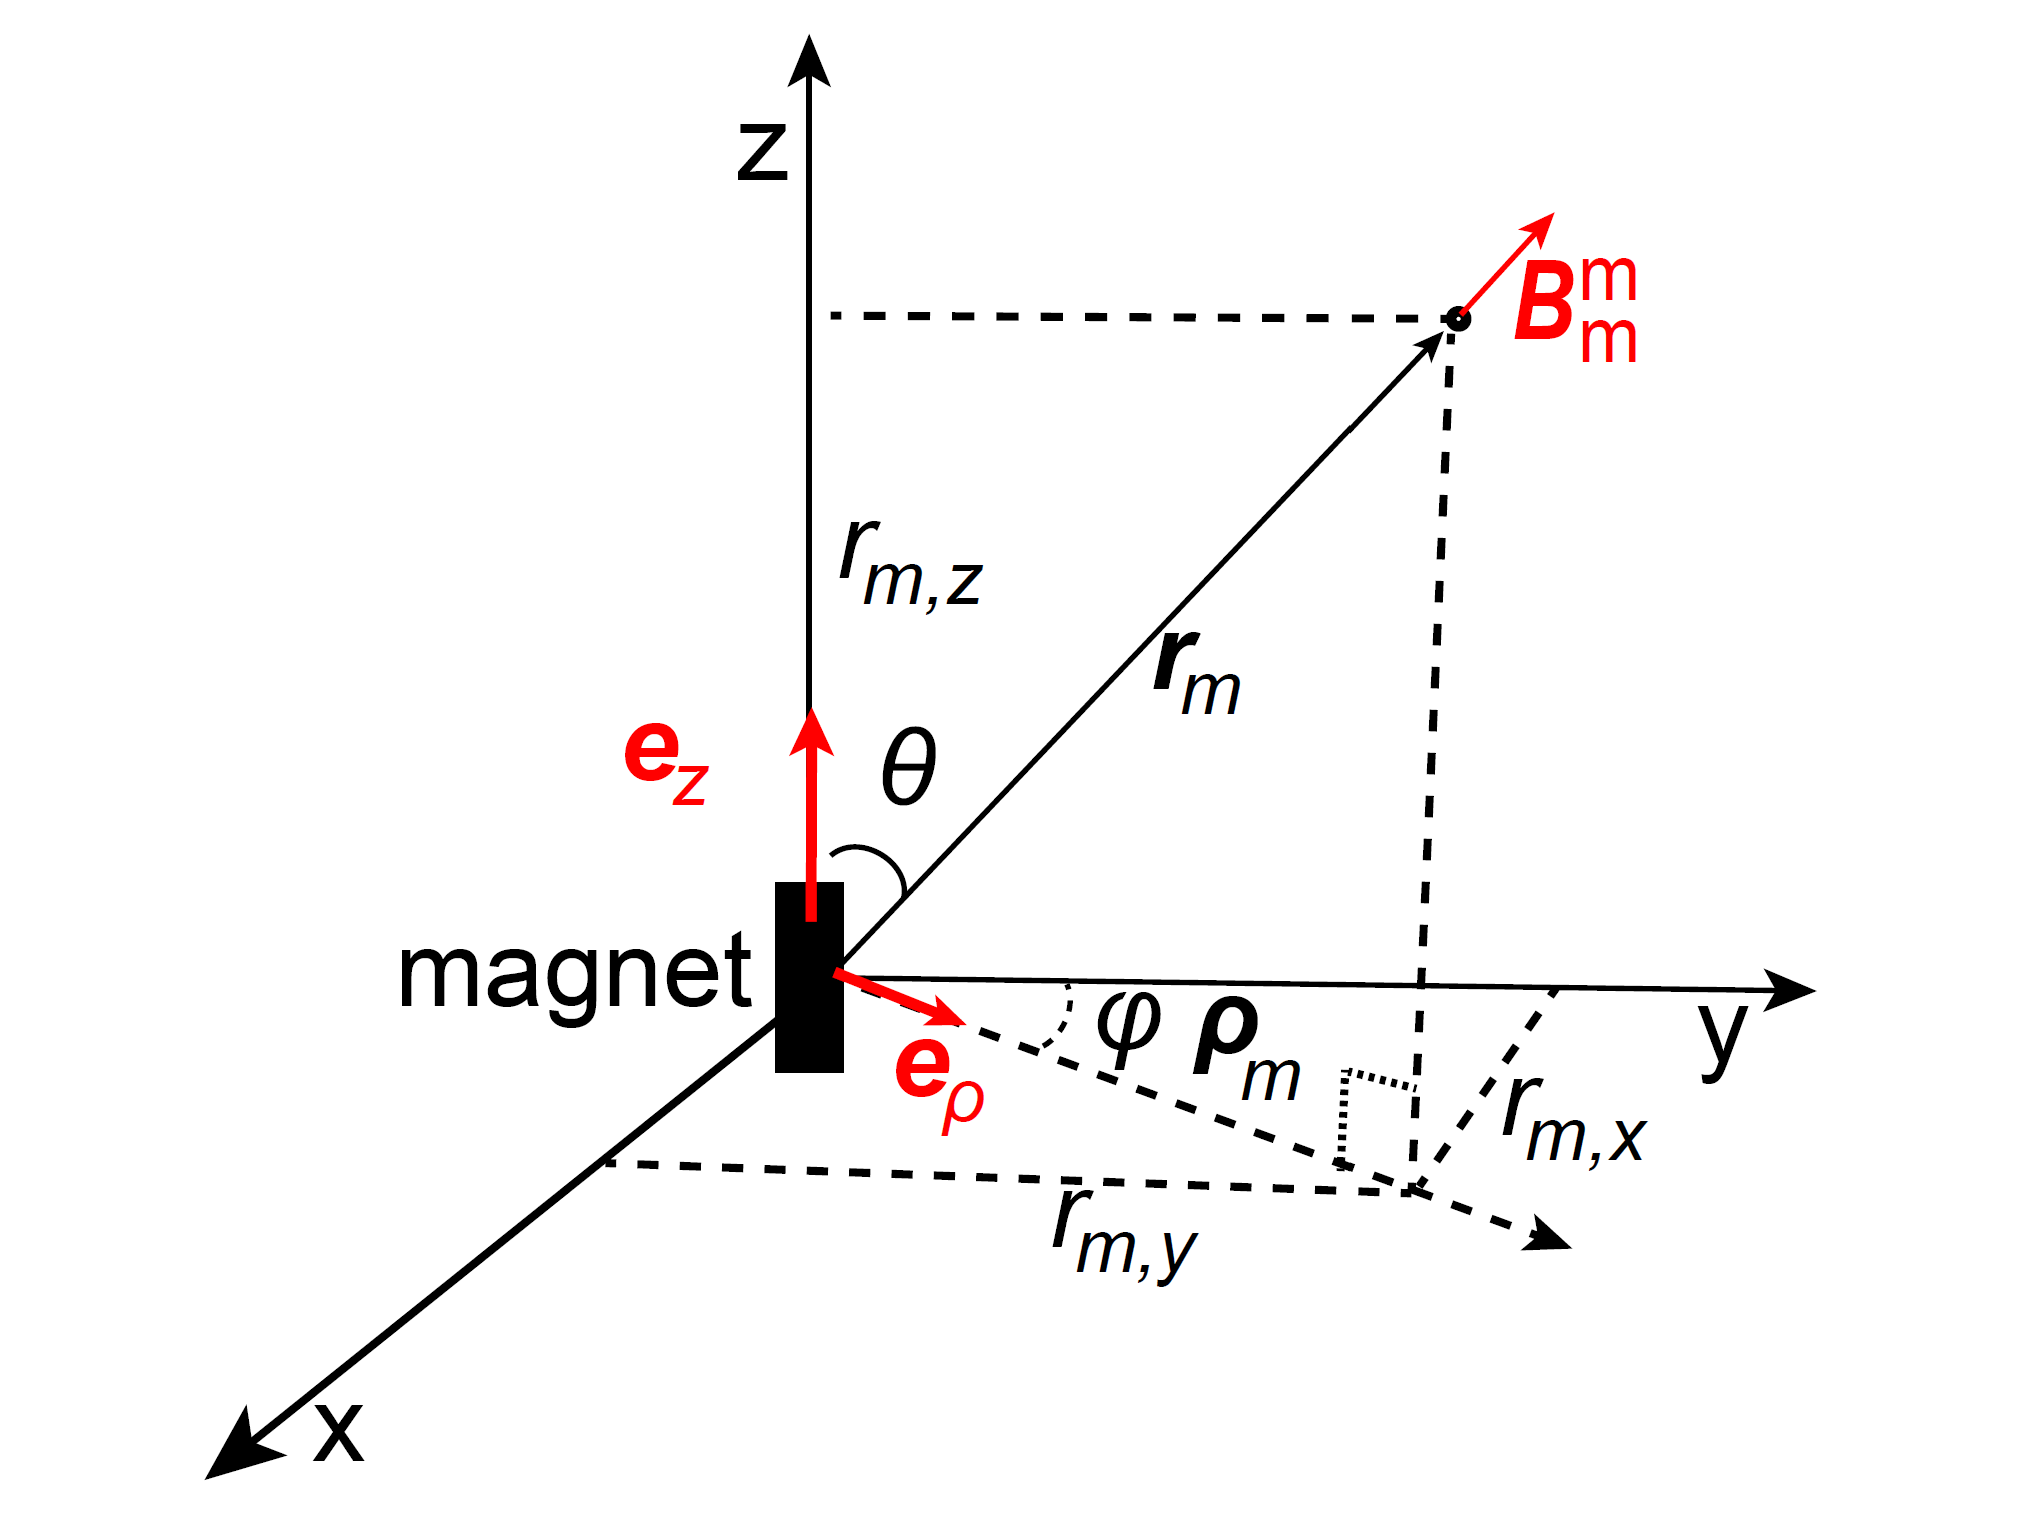
\includegraphics[width=.5\linewidth]{magnet/dipole-model-of-a-magnet.png}
    \caption{\label{fig:dipole-model-of-a-magnet}Dipole Model of a Magnet}
\end{figure}

\begin{equation}
    \label{equ:dipole-model}
    f(r_m, \theta) = \frac{\mu_0 M_m}{4\pi r_m^3}[\frac{3}{2}\sin{2\theta}\vec{e_p} + (3\cos^2{\theta} - 1)\vec{e_z}]
\end{equation}
其中,$\mu_0$是真空磁导率,$M_m$是磁偶极矩强度。
$r_m$是传感器在磁体坐标系中的位置,以球坐标系表示,如\autoref{equ:spherical-coordinate-system}所示:
\begin{equation}
    \label{equ:spherical-coordinate-system}
    r_{m,x} = r_m\cos{\theta}\sin{\phi},\ r_{m,y} = r_m\cos{\theta}\cos{\phi},\ r_{m,z} = r_m\sin{\theta}
\end{equation}
其中,$(r_m, \theta, \phi)$表示径向距离、极角和方位角。$\vec{e}_{\rho}$和$\vec{e}_z$是$r_m$在水平平面上和垂直轴上的投影的单位向量,如\autoref{fig:dipole-model-of-a-magnet}所示。

当通过三轴磁传感器(TAM)测量位于位置$r_m$处的磁场时(用$y^s_{mag}$表示),这个测量可以用如\autoref{equ:dipole-measurement}所示的数学模型描述:
\begin{equation}
    \label{equ:dipole-measurement}
    y_{mag}^s = A(B_m^s + B_e^s + b) + n_{B}
\end{equation}
其中,$A$是包括灵敏度误差、非正交性误差和软铁效应误差在内的综合误差参数。
$b$是包括偏移误差和硬铁效应误差在内的综合误差。
$B_m^s$是磁铁产生的磁场。
$B_e^s$是包括地磁场和周围干扰在内的扰动磁场,$n_B$是测量噪声。
通过校准过程可以估计出$A$和$b$。当$|B_m^s|$远大于$|B_e^s|$时,\autoref{equ:dipole-measurement}可以被近似为\autoref{equ:simplified-dipole-measurement}:
\begin{equation}
    \label{equ:simplified-dipole-measurement}
    y_{mag}^s \approx A(B_m^s + b) + n_{B}
\end{equation}

\subsection{永磁体分析与校准}
为了保证后续手指追踪定位与手势识别的准确度,需要提前测量并标定永磁体的磁偶极矩强度,否则将无法通过相关的数学模型计算出手指相对于手背的位置,或者计算出的相对位置存在较大的偏差
在本毕业设计项目中,为实现此目标,我自行设计了一套标定永磁体磁偶极矩强度的装置,进行了相关的数学建模与分析,并最终使用回归模型对毕设项目中所使用的圆柱体永磁体的磁偶极矩强度进行了测量。
测量装置如\autoref{fig:magnet-measure-device}所示:

\begin{figure}[H]
    \centering
    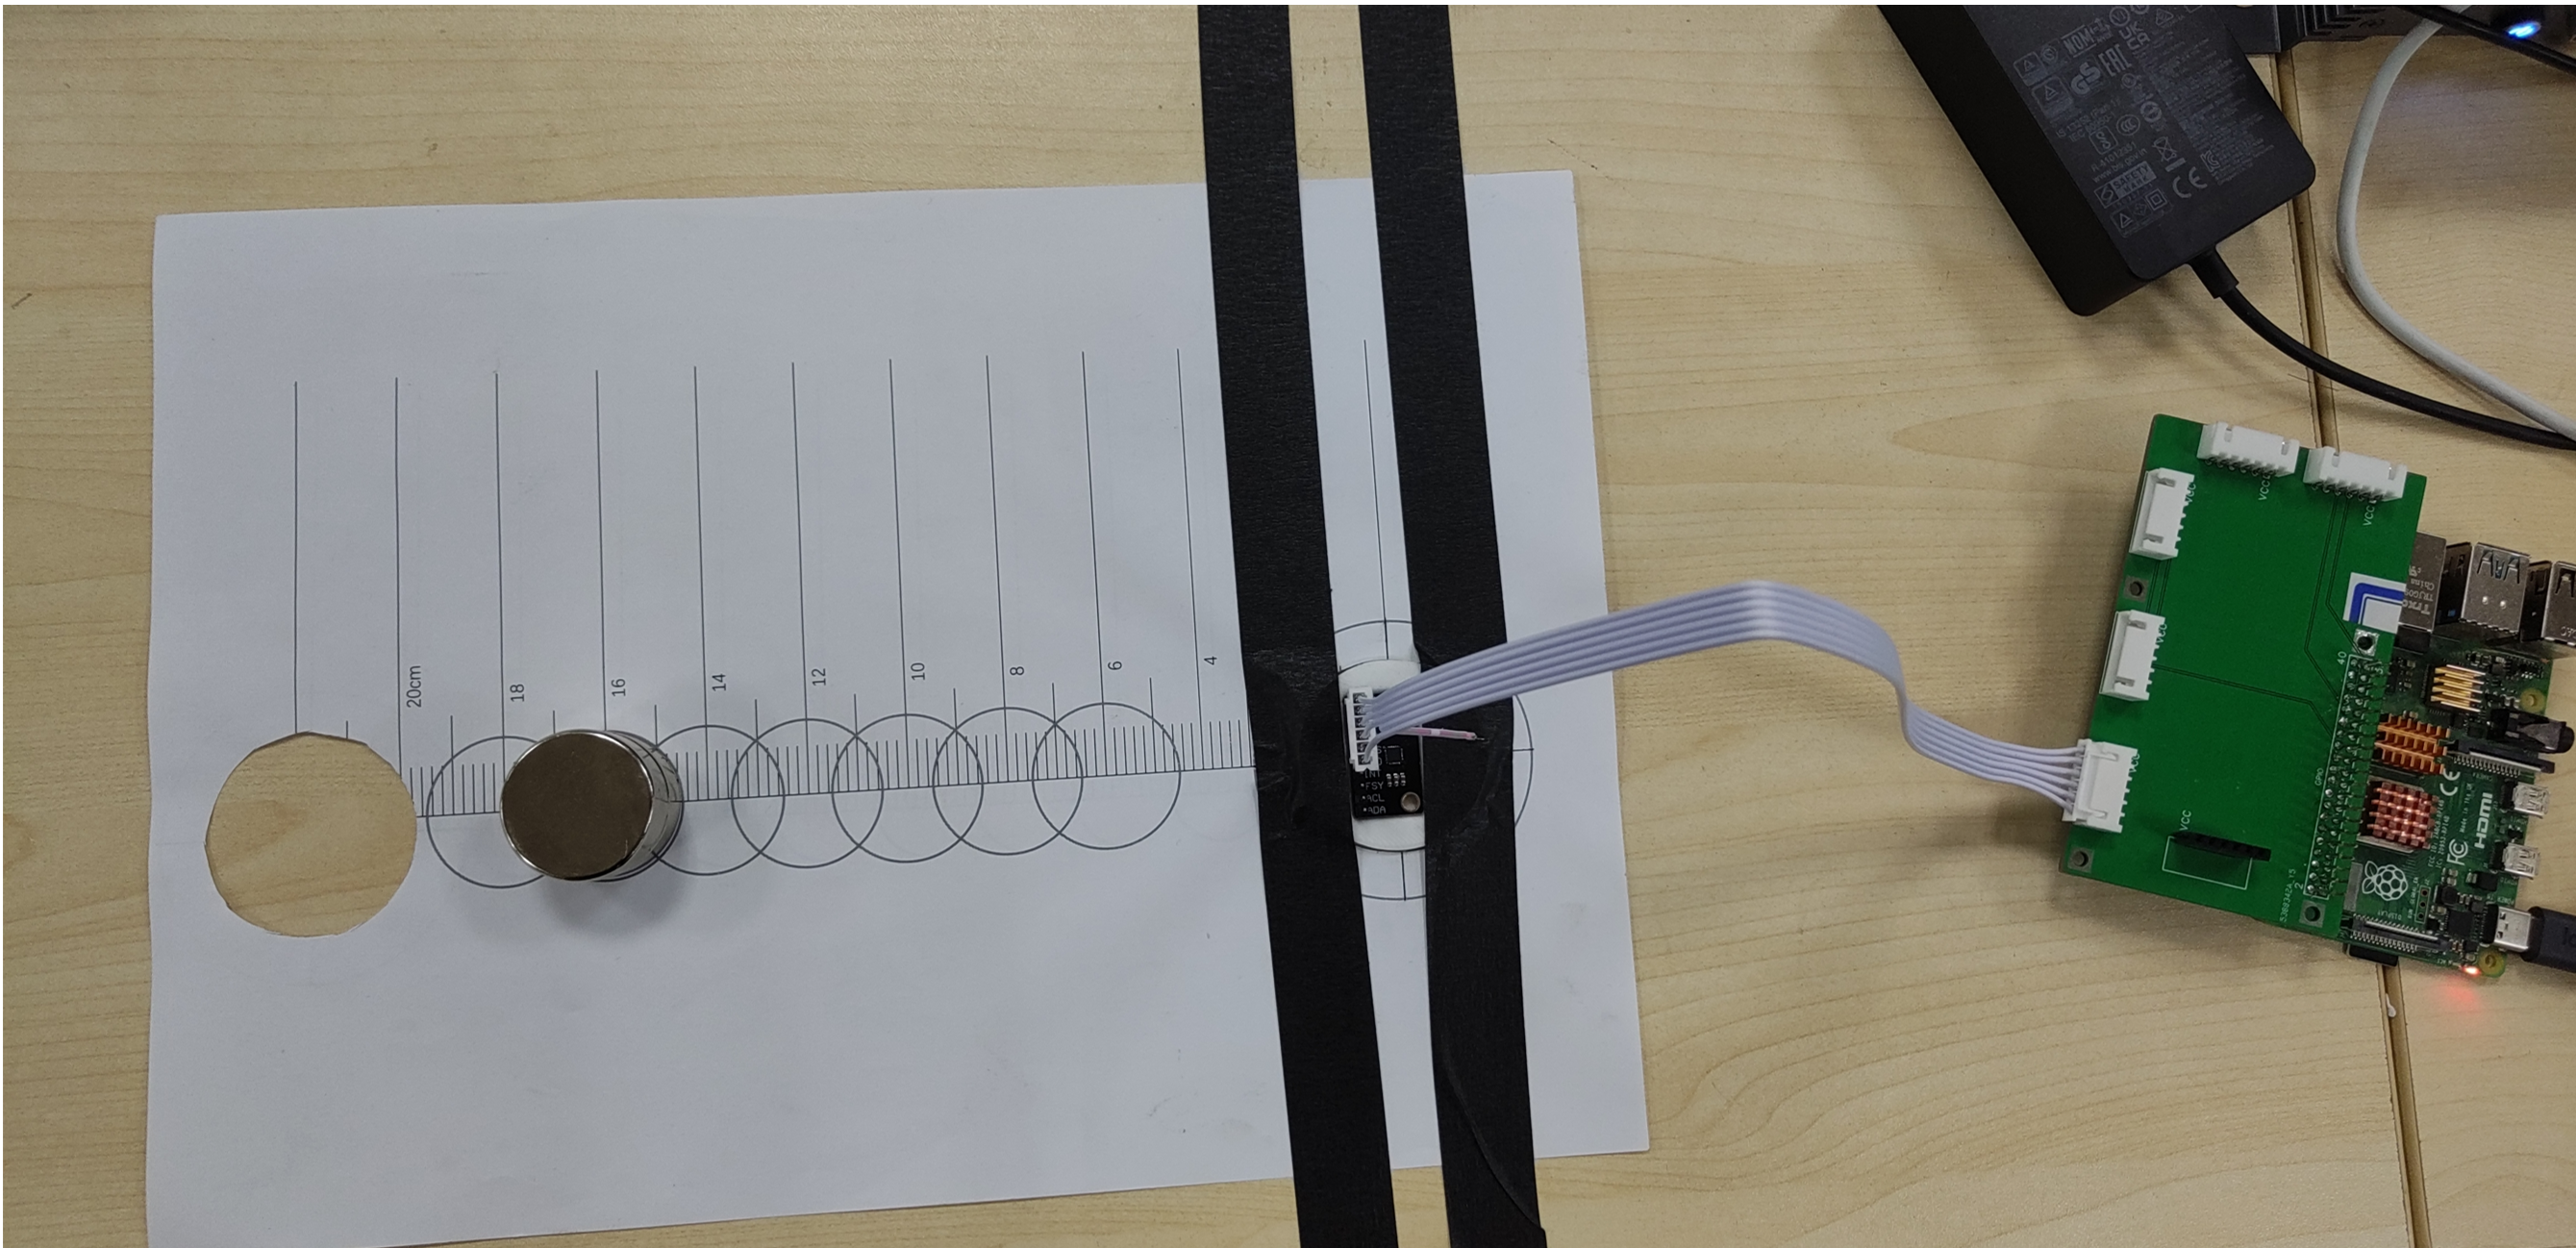
\includegraphics[width=.8\linewidth]{magnet/magnet-measure-device.png}
    \caption{\label{fig:magnet-measure-device}Magnetic Field Measurement Device}
\end{figure}

\subsubsection{数据采集与记录}
为准确测定永磁体的磁偶极矩强度,本毕设项目使用如下方法测量并记录相关数据:

首先,将一个磁传感器固定在实验室桌面上,并附上1张有距离刻度的测量纸。随后,按如下步骤进行测量并记录数据:
\begin{enumerate}
    \item 确认周围无其它磁场环境干扰后,用磁传感器测出当前的地磁强度并进行记录
    \item 在多个不同距离处测量永磁体在磁传感器位置的磁场感应强度并进行记录(使用带有距离刻度的测量纸进行读数)
\end{enumerate}

测量结果如\autoref{fig:permanent-magnet-analysis-g}所示。其中,纵坐标为在测量纸上读得的当前永磁体与磁传感器的距离,横坐标为磁传感器所测得的磁场感应强度的模长。

\begin{figure}[H]
    \centering
    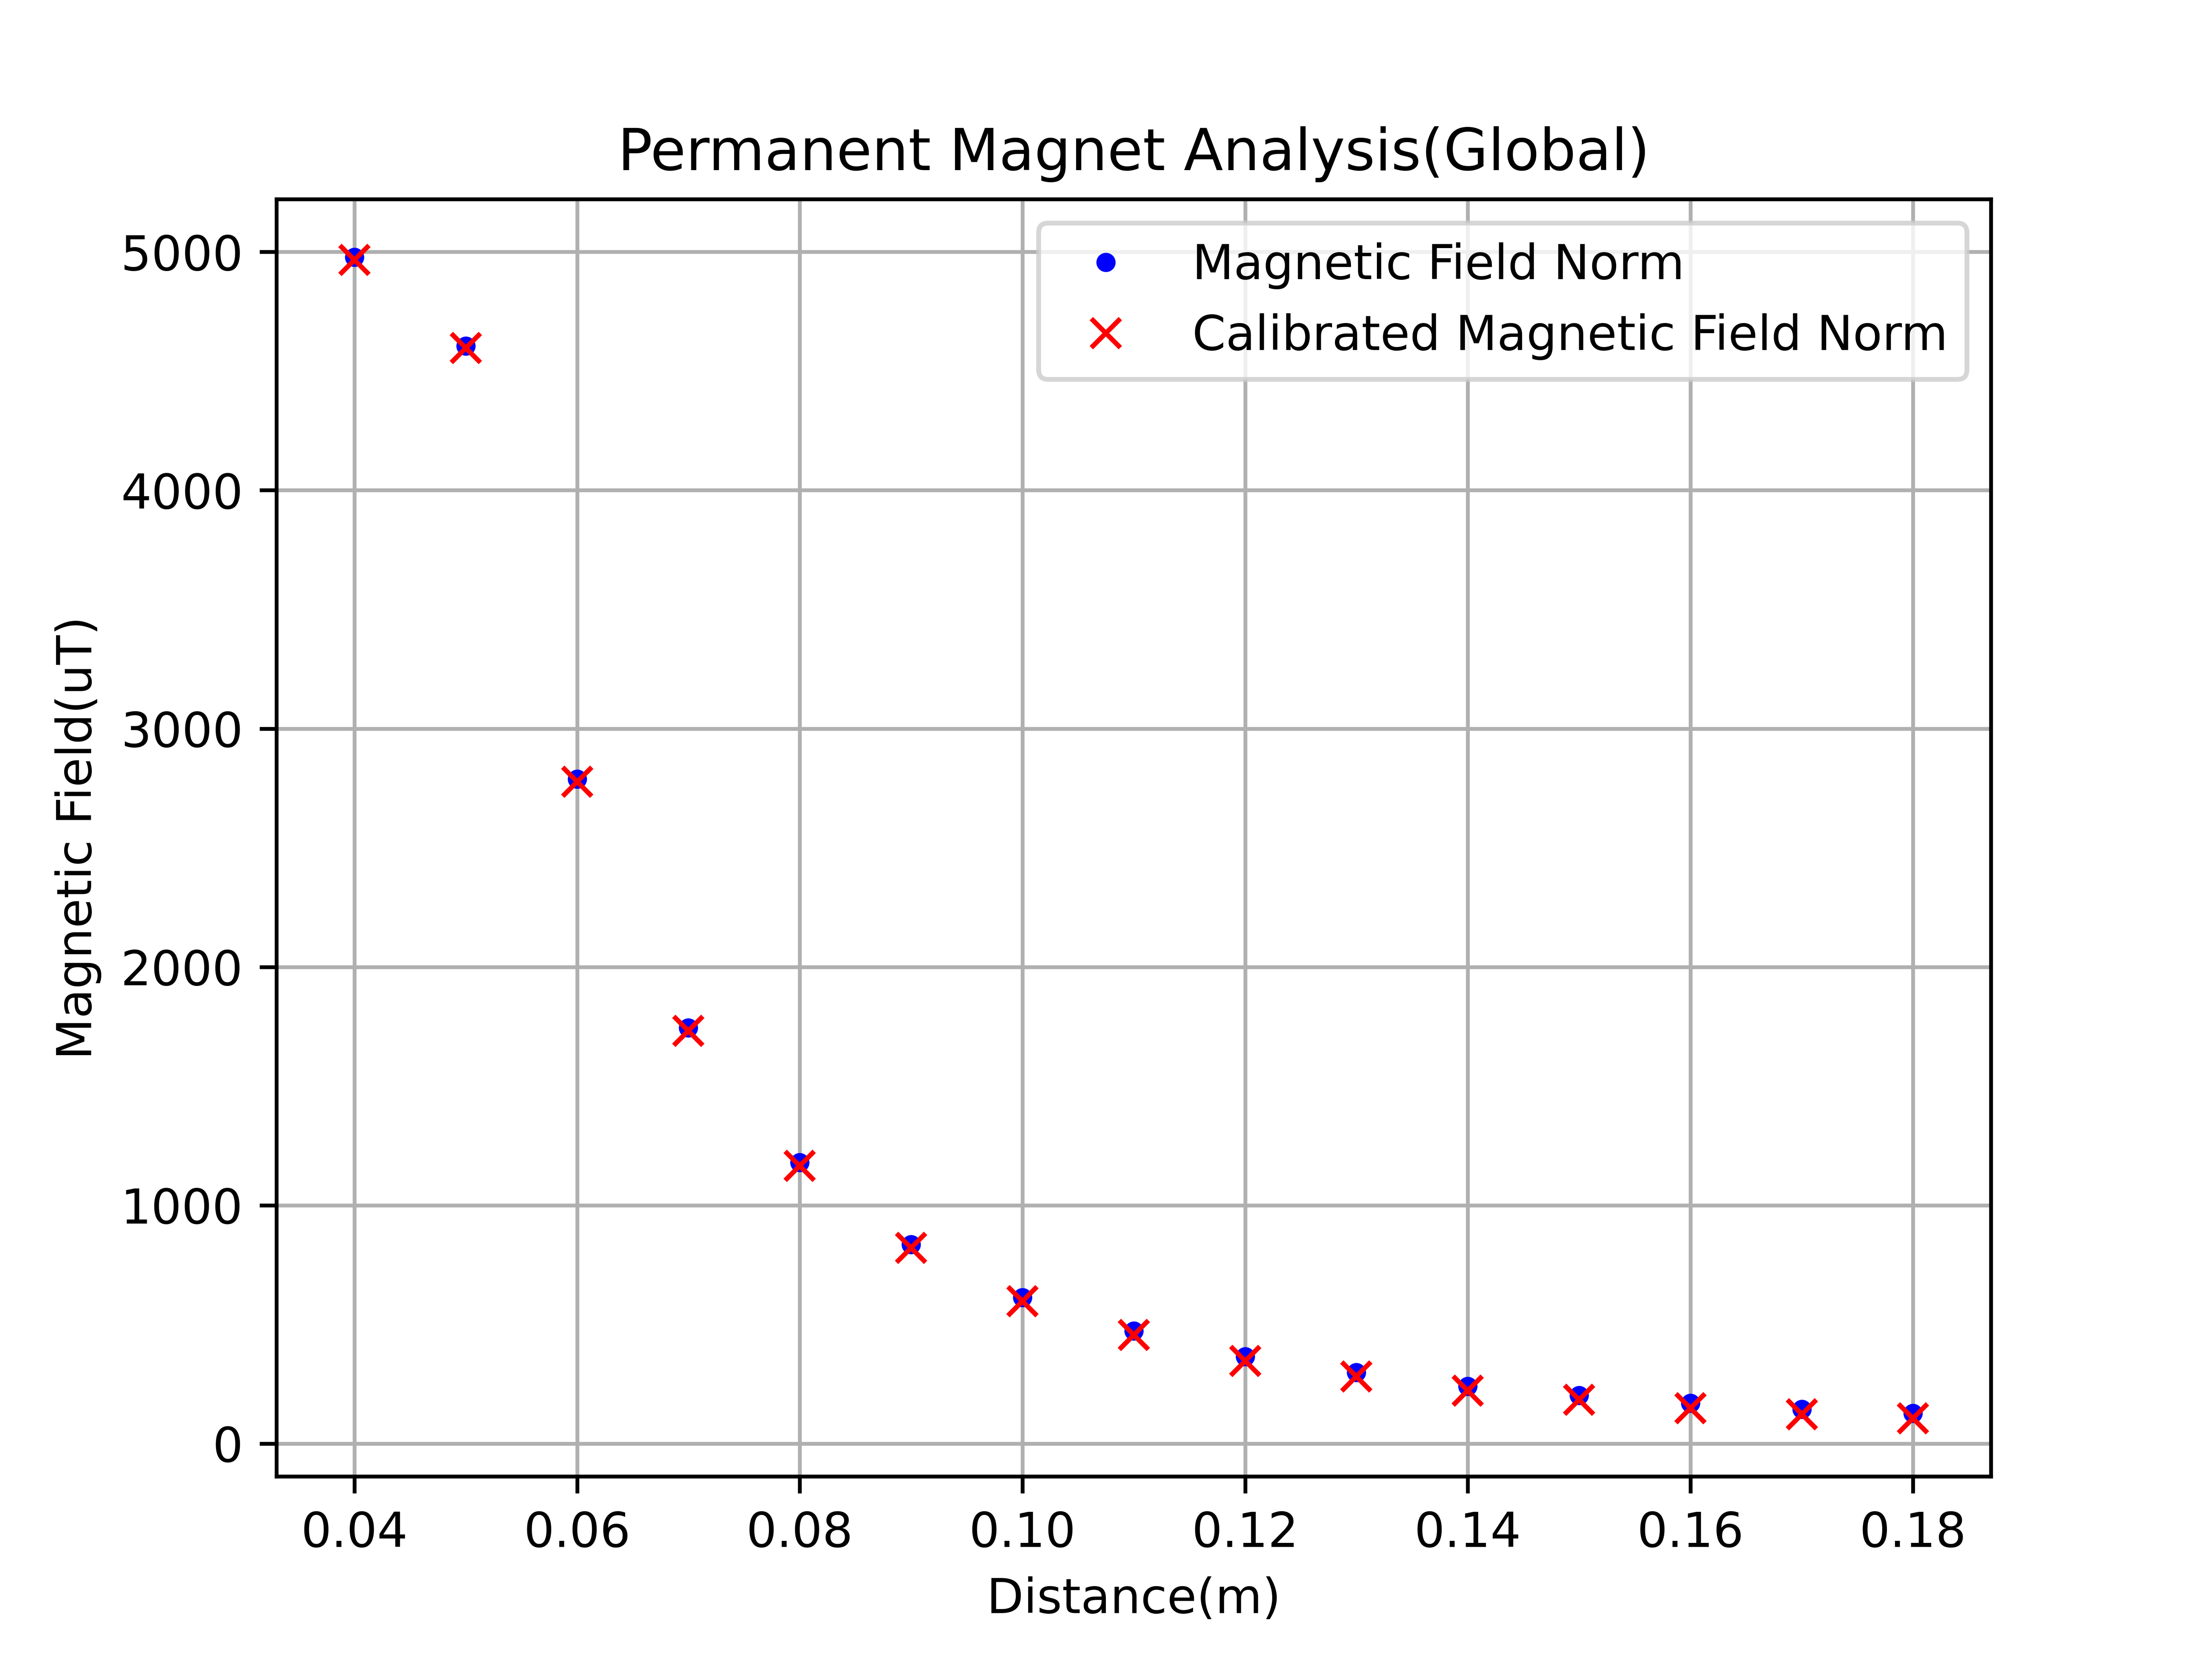
\includegraphics[width=.6\linewidth]{magnet/permanent-magnet-analysis-g.png}
    \caption{\label{fig:permanent-magnet-analysis-g}Permanent Magnet Analysis (Global)}
\end{figure} 

在\autoref{fig:permanent-magnet-analysis-g}中,蓝色的点表示未去掉地磁场影响时磁传感器所测得的磁场感应强度的模长,红色的叉则表示去掉地磁场影响之后的相应结果。
相应的回归计算及误差分析过程见下一节。

\subsubsection{数学建模与回归计算}
首先,因为在测量时,永磁体与磁传感器位于同一个平面上,故可直接令\autoref{equ:dipole-model}中的$\theta = \frac{\pi}{2}$。随后,对\autoref{equ:dipole-model}取模,可得\autoref{equ:norm-dipole-model}:
\begin{equation}
    \label{equ:norm-dipole-model}
    |f(r_m, \theta)| = \frac{\mu_0 M_m}{4\pi r_m^3}\ \ (\theta = \frac{\pi}{2})
\end{equation}

由于永磁体与磁传感器之间的距离由测量纸上的刻度读出,故其与两者之间的真实距离存在系统误差。记此系统误差为$\widehat{d}$,待测永磁体的磁偶极矩强度为$\widehat{M_m}$,建立回归模型\autoref{equ:regression-norm-dipole-model}:
\begin{equation}
    \label{equ:regression-norm-dipole-model}
    F(x, \widehat{M_m}, \widehat{d}) = \frac{\mu_0 \widehat{M_m}}{4\pi(x+\widehat{d})^3} \ (\theta = \frac{\pi}{2})
\end{equation}
其中,$\widehat{d}$和$\widehat{M_m}$为待进行回归计算的估计量。
将上一节中测得并记录的数据代入,进行回归计算,可得\autoref{equ:regression-norm-dipole-model-result}:
\begin{equation}
    \label{equ:regression-norm-dipole-model-result}
    \begin{aligned}
    F(x, \widehat{M_m}, \widehat{d}) &= \frac{\mu_0 \widehat{M_m}}{4\pi(x+\widehat{d})^3} \ (\theta = \frac{\pi}{2}) \\
    & \Longrightarrow \widehat{M_m} \approx 5.98 A\cdot m^2, \widehat{d} \approx 0.01m
    \end{aligned}
\end{equation}
由此可知,本毕设项目中使用的永磁体的磁偶极矩强度约为$5.98 A\cdot m^2$。

上述回归计算的最终效果如\autoref{fig:dipole-model-regression-with-calibrated-magnetic-field-g}所示:

\begin{figure}[H]
    \centering
    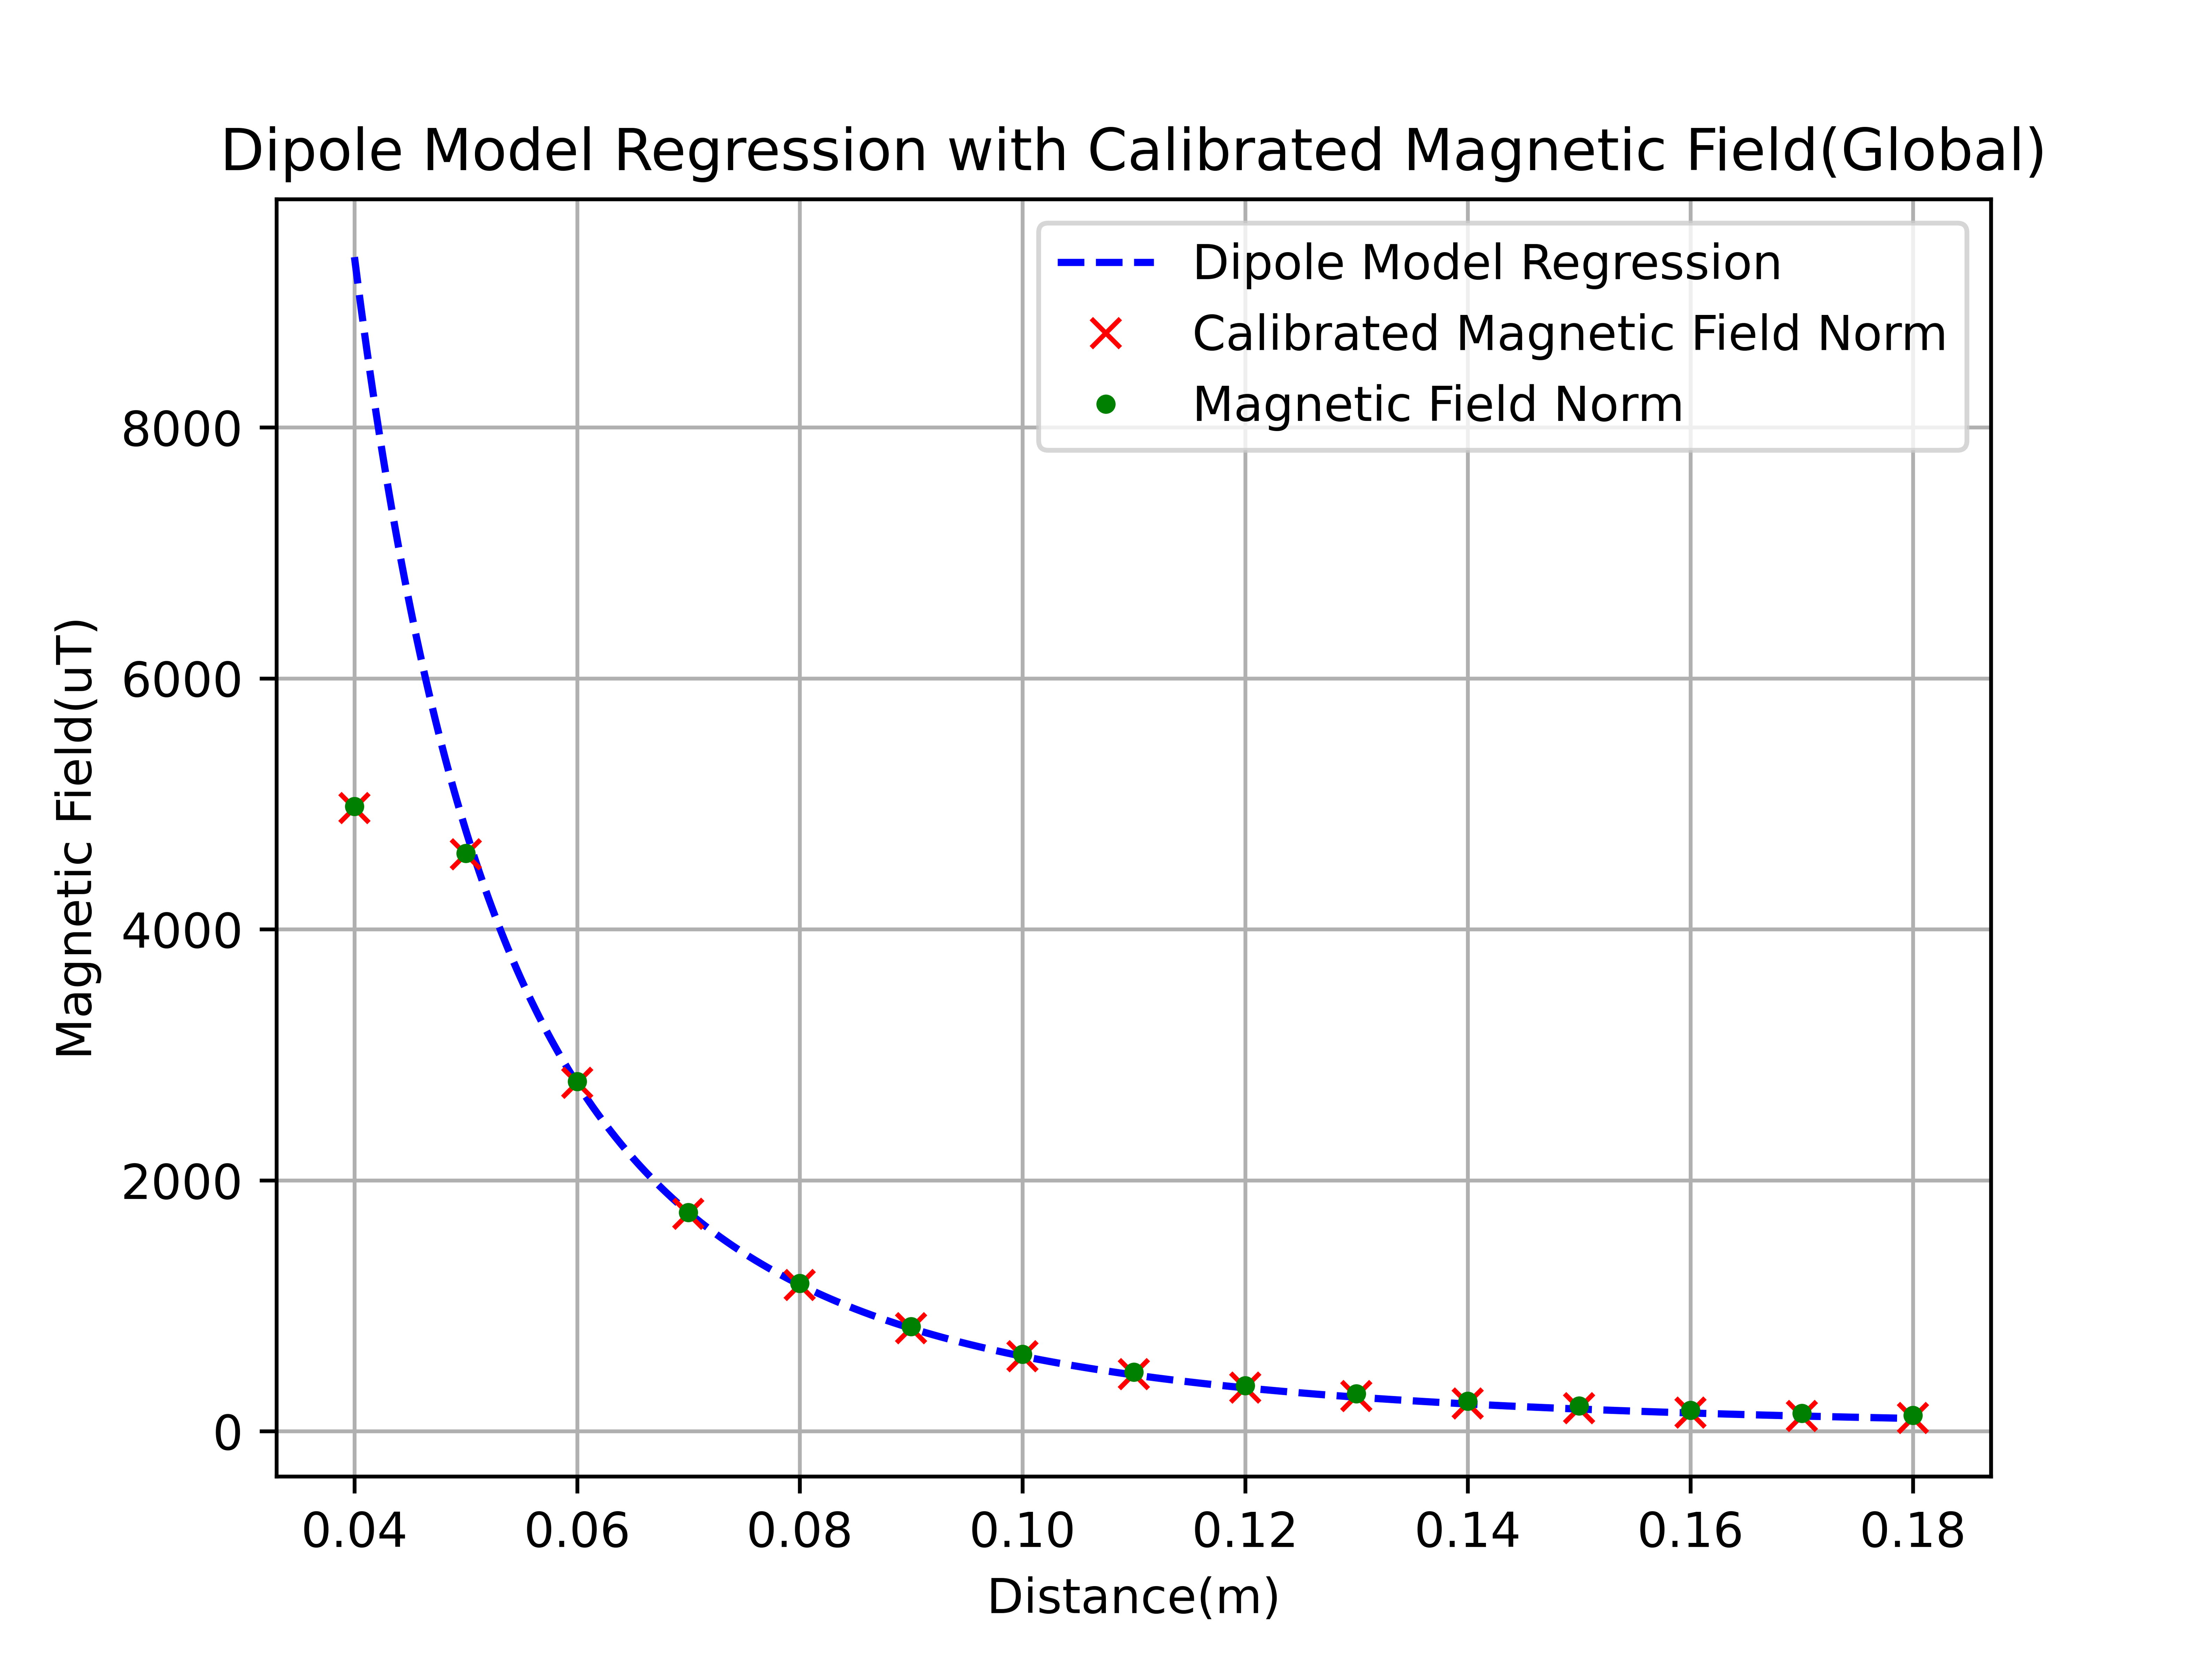
\includegraphics[width=.6\linewidth]{magnet/dipole-model-regression-with-calibrated-magnetic-field-g.png}
    \caption{\label{fig:dipole-model-regression-with-calibrated-magnetic-field-g}Dipole Model Regression (Global)}
\end{figure}

相对误差分析如\autoref{fig:relative-error-rate-under-effect-of-geomagnetic-field}所示:

\begin{figure}[H]
    \centering
    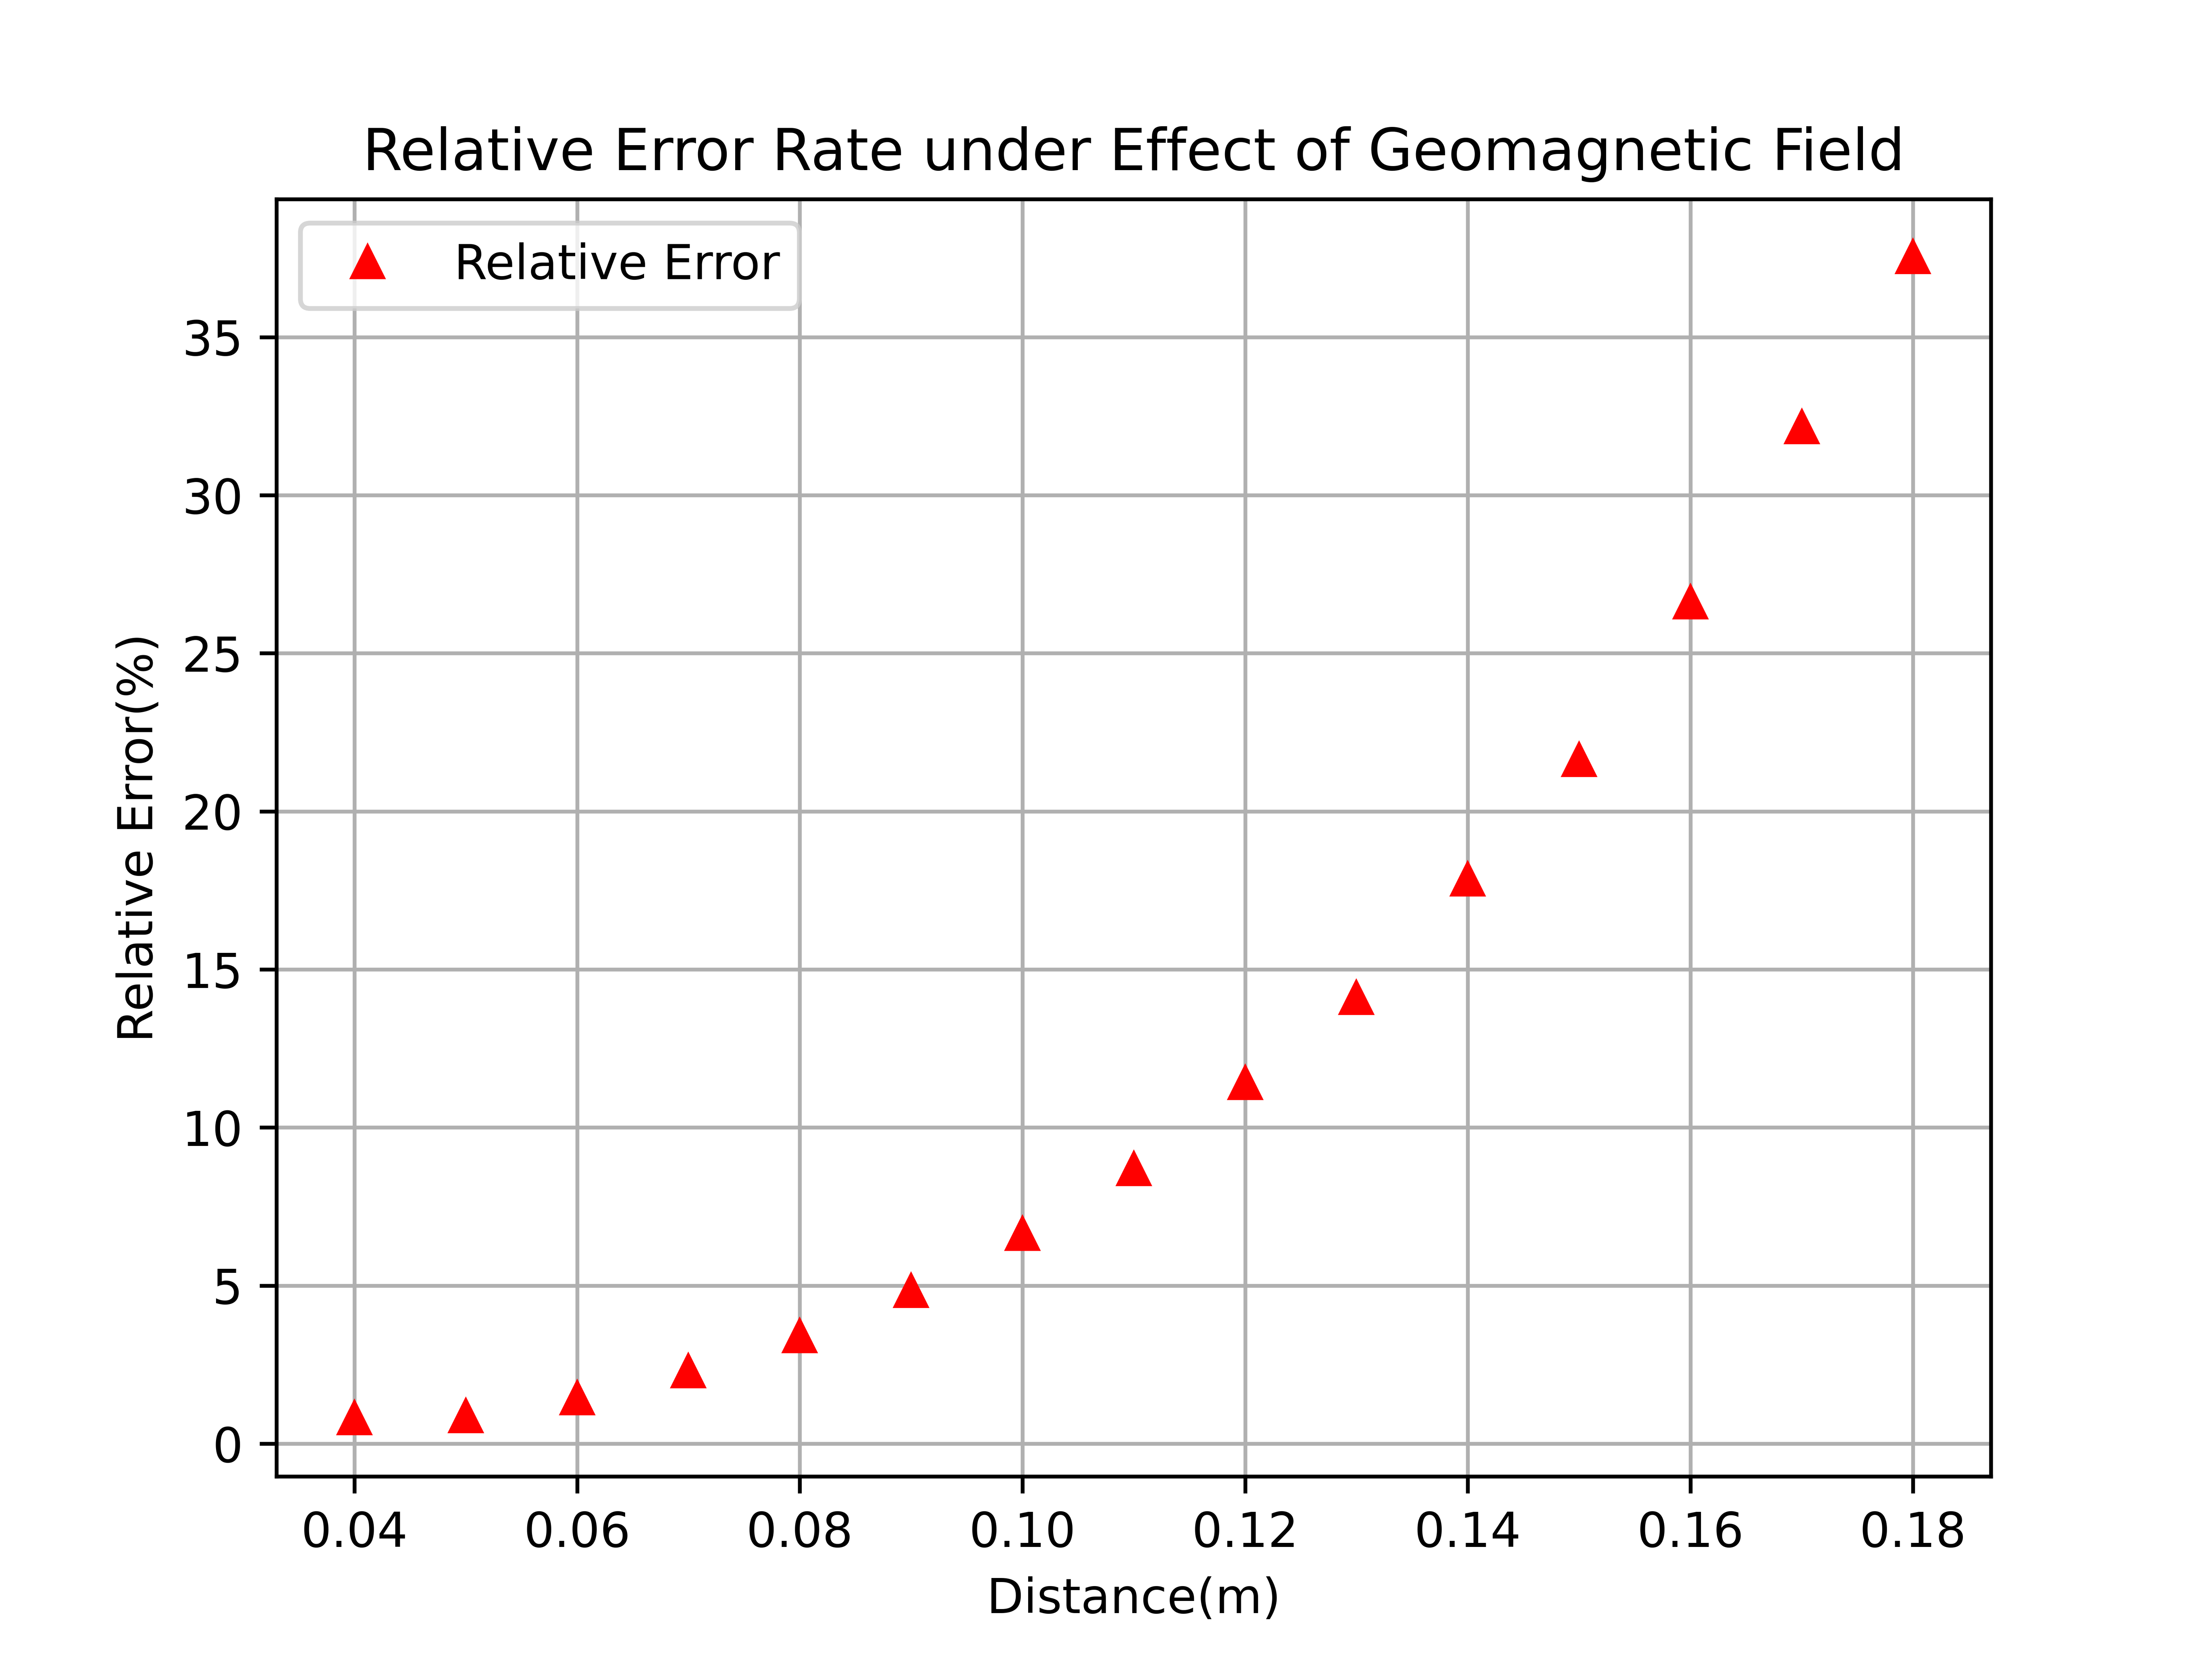
\includegraphics[width=.6\linewidth]{magnet/relative-error-rate-under-effect-of-geomagnetic-field.png}
    \caption{\label{fig:relative-error-rate-under-effect-of-geomagnetic-field}Relative Error Under Geomagnetic Field}
\end{figure}

在指尖距离手背的有效距离范围内(0.06m-0.15m),地磁场的干扰可以被忽略(见\autoref{fig:relative-error-rate-under-effect-of-geomagnetic-field});
当磁传感器与所选用的永磁体之间的距离小于0.05m时,磁传感器的测量结果饱和(±4700 μT),如\autoref{fig:dipole-model-regression-with-calibrated-magnetic-field-g}所示。

\subsection{相对位置计算}
\subsubsection{数学建模与非线性方程组求解}
当指尖传感器与手背的相对姿态$C_m^s$已知时,可以根据\autoref{equ:simplified-dipole-measurement}将磁传感器的测量输出旋转到磁铁(手背)坐标系。然后根据\autoref{equ:simplified-dipole-measurement}将$B_m^m$表示为\autoref{equ:rotated-dipole-measurement}:
\begin{equation}
    \label{equ:rotated-dipole-measurement}
    B_m^m = (C_m^s)^{-1}(A^{-1}y_{mag}^s - b)
\end{equation}
接下来,基于\autoref{equ:dipole-model},已知相对姿态$C^s_m$和$B_m^m$,可以通过求解一个非线性优化问题来估计相对位置$r_m$(如\autoref{fig:dipole-model-coordinate}所示)~\cite{mainArticle2}。优化问题的目标函数定义如\autoref{equ:r-theta-dipole-model-equation}所示:
\begin{equation}
    \label{equ:r-theta-dipole-model-equation}
    \begin{cases}
        (r_m, \theta) = argmin{||g||}_2^2 \\
        g = f(r_m, \theta) - (B_{m,h}^m,B_{m,z}^m)
    \end{cases}
\end{equation}
其中,$B_{m,h}^m$和$B_{m,z}^m$分别表示$B_m^m$的水平和垂直分量的强度。

\begin{figure}[H]
    \centering
    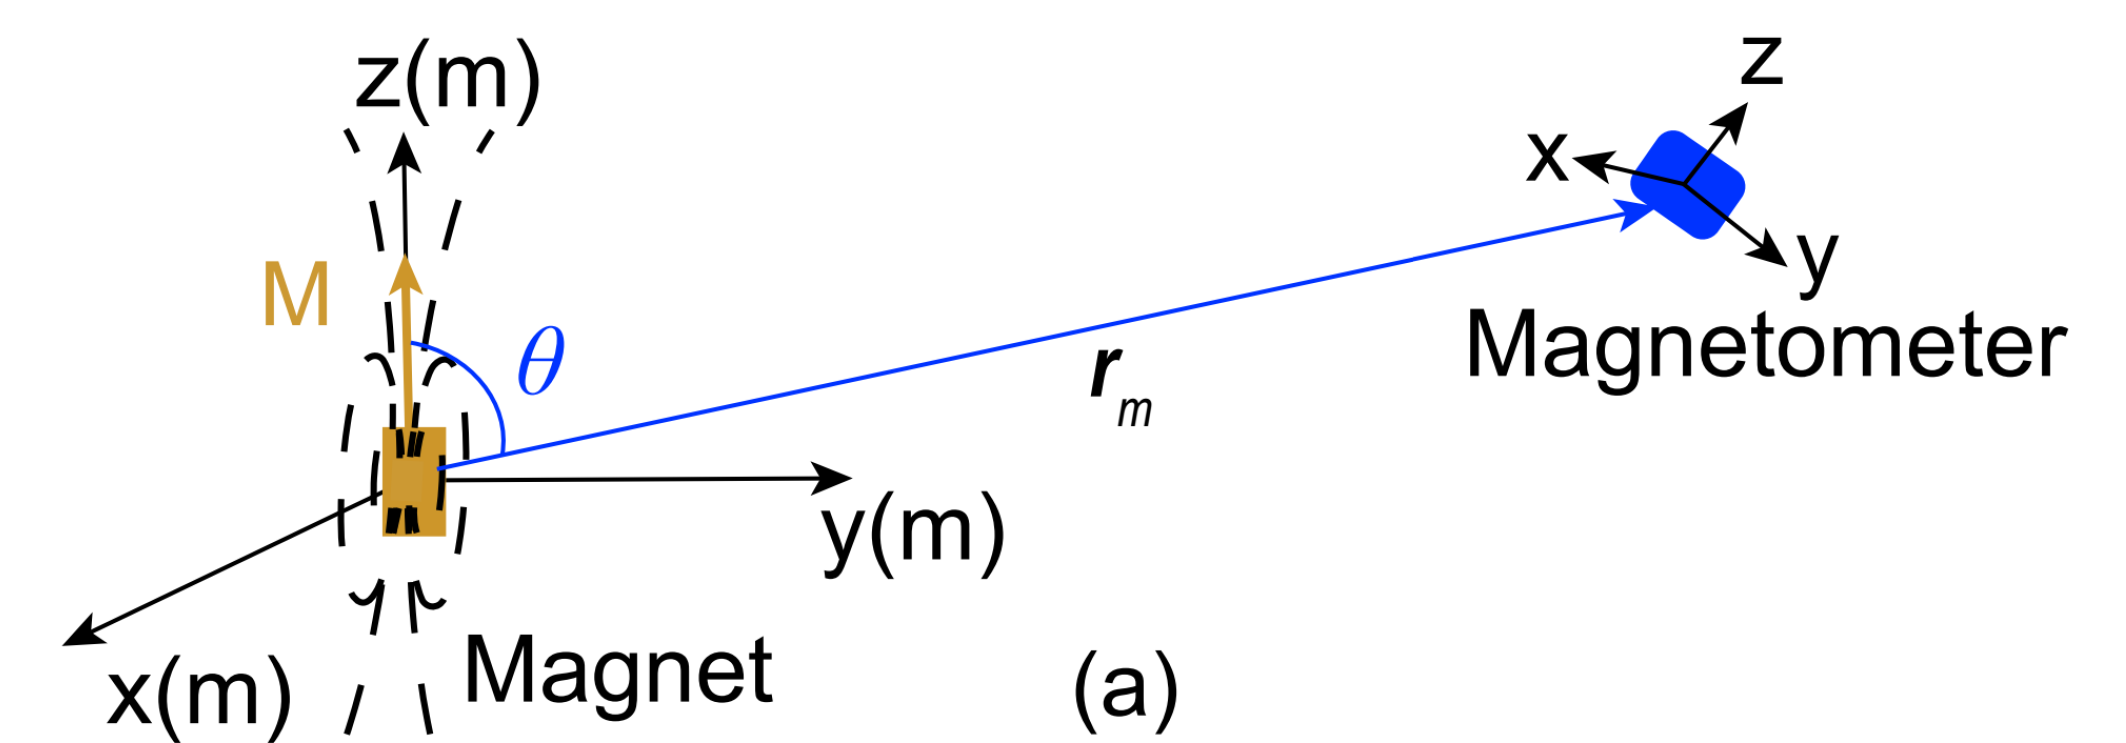
\includegraphics[width=.7\linewidth]{magnet/dipole-model-coordinate.png}
    \caption{\label{fig:dipole-model-coordinate}Magnet in the Center of A Coordinate System}
\end{figure}

显然,这是一个非线性优化问题,可以使用数值分析中的方法进行迭代求解。
\subsubsection{手动计算雅各比矩阵}
为快速、准确地求解上节中所描述的非线性方程组,在对此方程组及其解的特征进行分析后,本次毕设项目最终使用了Trust Region Reflective Algorithm来迭代求解此非线性方程组,从而计算出手指相对于手背的相对位置
为进一步提高此算法的收敛概率与收敛速度,该线性方程组的雅各比矩阵被手动求出(如\autoref{equ:manual-jacobian-matrix}所示)并应用于求解器中。
\begin{equation}
    \label{equ:manual-jacobian-matrix}
    J_g = \frac{\partial{f}}{\partial{{(r_m, \theta)}_m}} = [\frac{\partial{f(r_m,\theta)}}{\partial{r_m}}\ \ \frac{\partial{f(r_m,\theta)}}{\partial{\theta}}]
\end{equation}

以下是本次毕设使用Python中的Scipy包利用Trust Region Reflective Algorithm求解此非线性方程组的核心代码,如\autoref{code:solve-dipole-model-equation}所示
\begin{lstlisting}[%
    language={Python},
    caption={Solve Dipole Model},
    label={code:solve-dipole-model-equation}
]
from scipy.optimize import least_squares
import numpy as np
...
# Define least equation
def equationFunction(x, magRou, magZ):
    return np.array([K * 3 * np.sin(2 * x[1]) / (2 * np.power(x[0], 3)) - magRou, K * (3 * np.cos(2 * x[1]) + 1 ) / (2 * np.power(x[0], 3)) - magZ])
# Define Jacobian matrix
def calculate_jac(x):
    return np.array([
        [-9 * K * np.sin(2 * x[1]) / (2 * np.power(x[0], 4)), 3 * K * np.cos(2 * x[1]) / np.power(x[0], 3)],
        [-3 * K * (3 * np.cos(2 * x[1]) + 1) / (2 * np.power(x[0], 4)), -3 * K * np.sin(2 * x[1]) / np.power(x[0], 3)]
    ])
...
# Solve equation with bounds limit
result = least_squares((lambda x : equationFunction(x, magRou, magZ)), initX, calculate_jac, bounds=([0, 0], [np.inf, np.pi / 2]))
\end{lstlisting}

\subsection{实时性能}
配合前几章中详述的此毕设项目中自行开发的库,使用Python中的Scipy包在树莓派4B平台上利用Trust Region Reflective Algorithm实时求解多个手指传感器相对于手背的相对位置,最终获得的相对位置更新速率大于50Hz。

\cleardoublepage
\section{动态追踪与手势识别}
\subsection{针对多个手指的动态位置追踪}
如上一章所述,通过软硬件之间的紧密协作与配合,整体系统能够以超过50Hz的频率实时求解5个位于指尖的传感器相对于手背的位置。
对于每一个位于手套指尖的传感器而言,对其求解得到的$r_m$与$\theta$如\autoref{fig:solved-r-theta-diagram}所示

\begin{figure}[H]
    \centering
    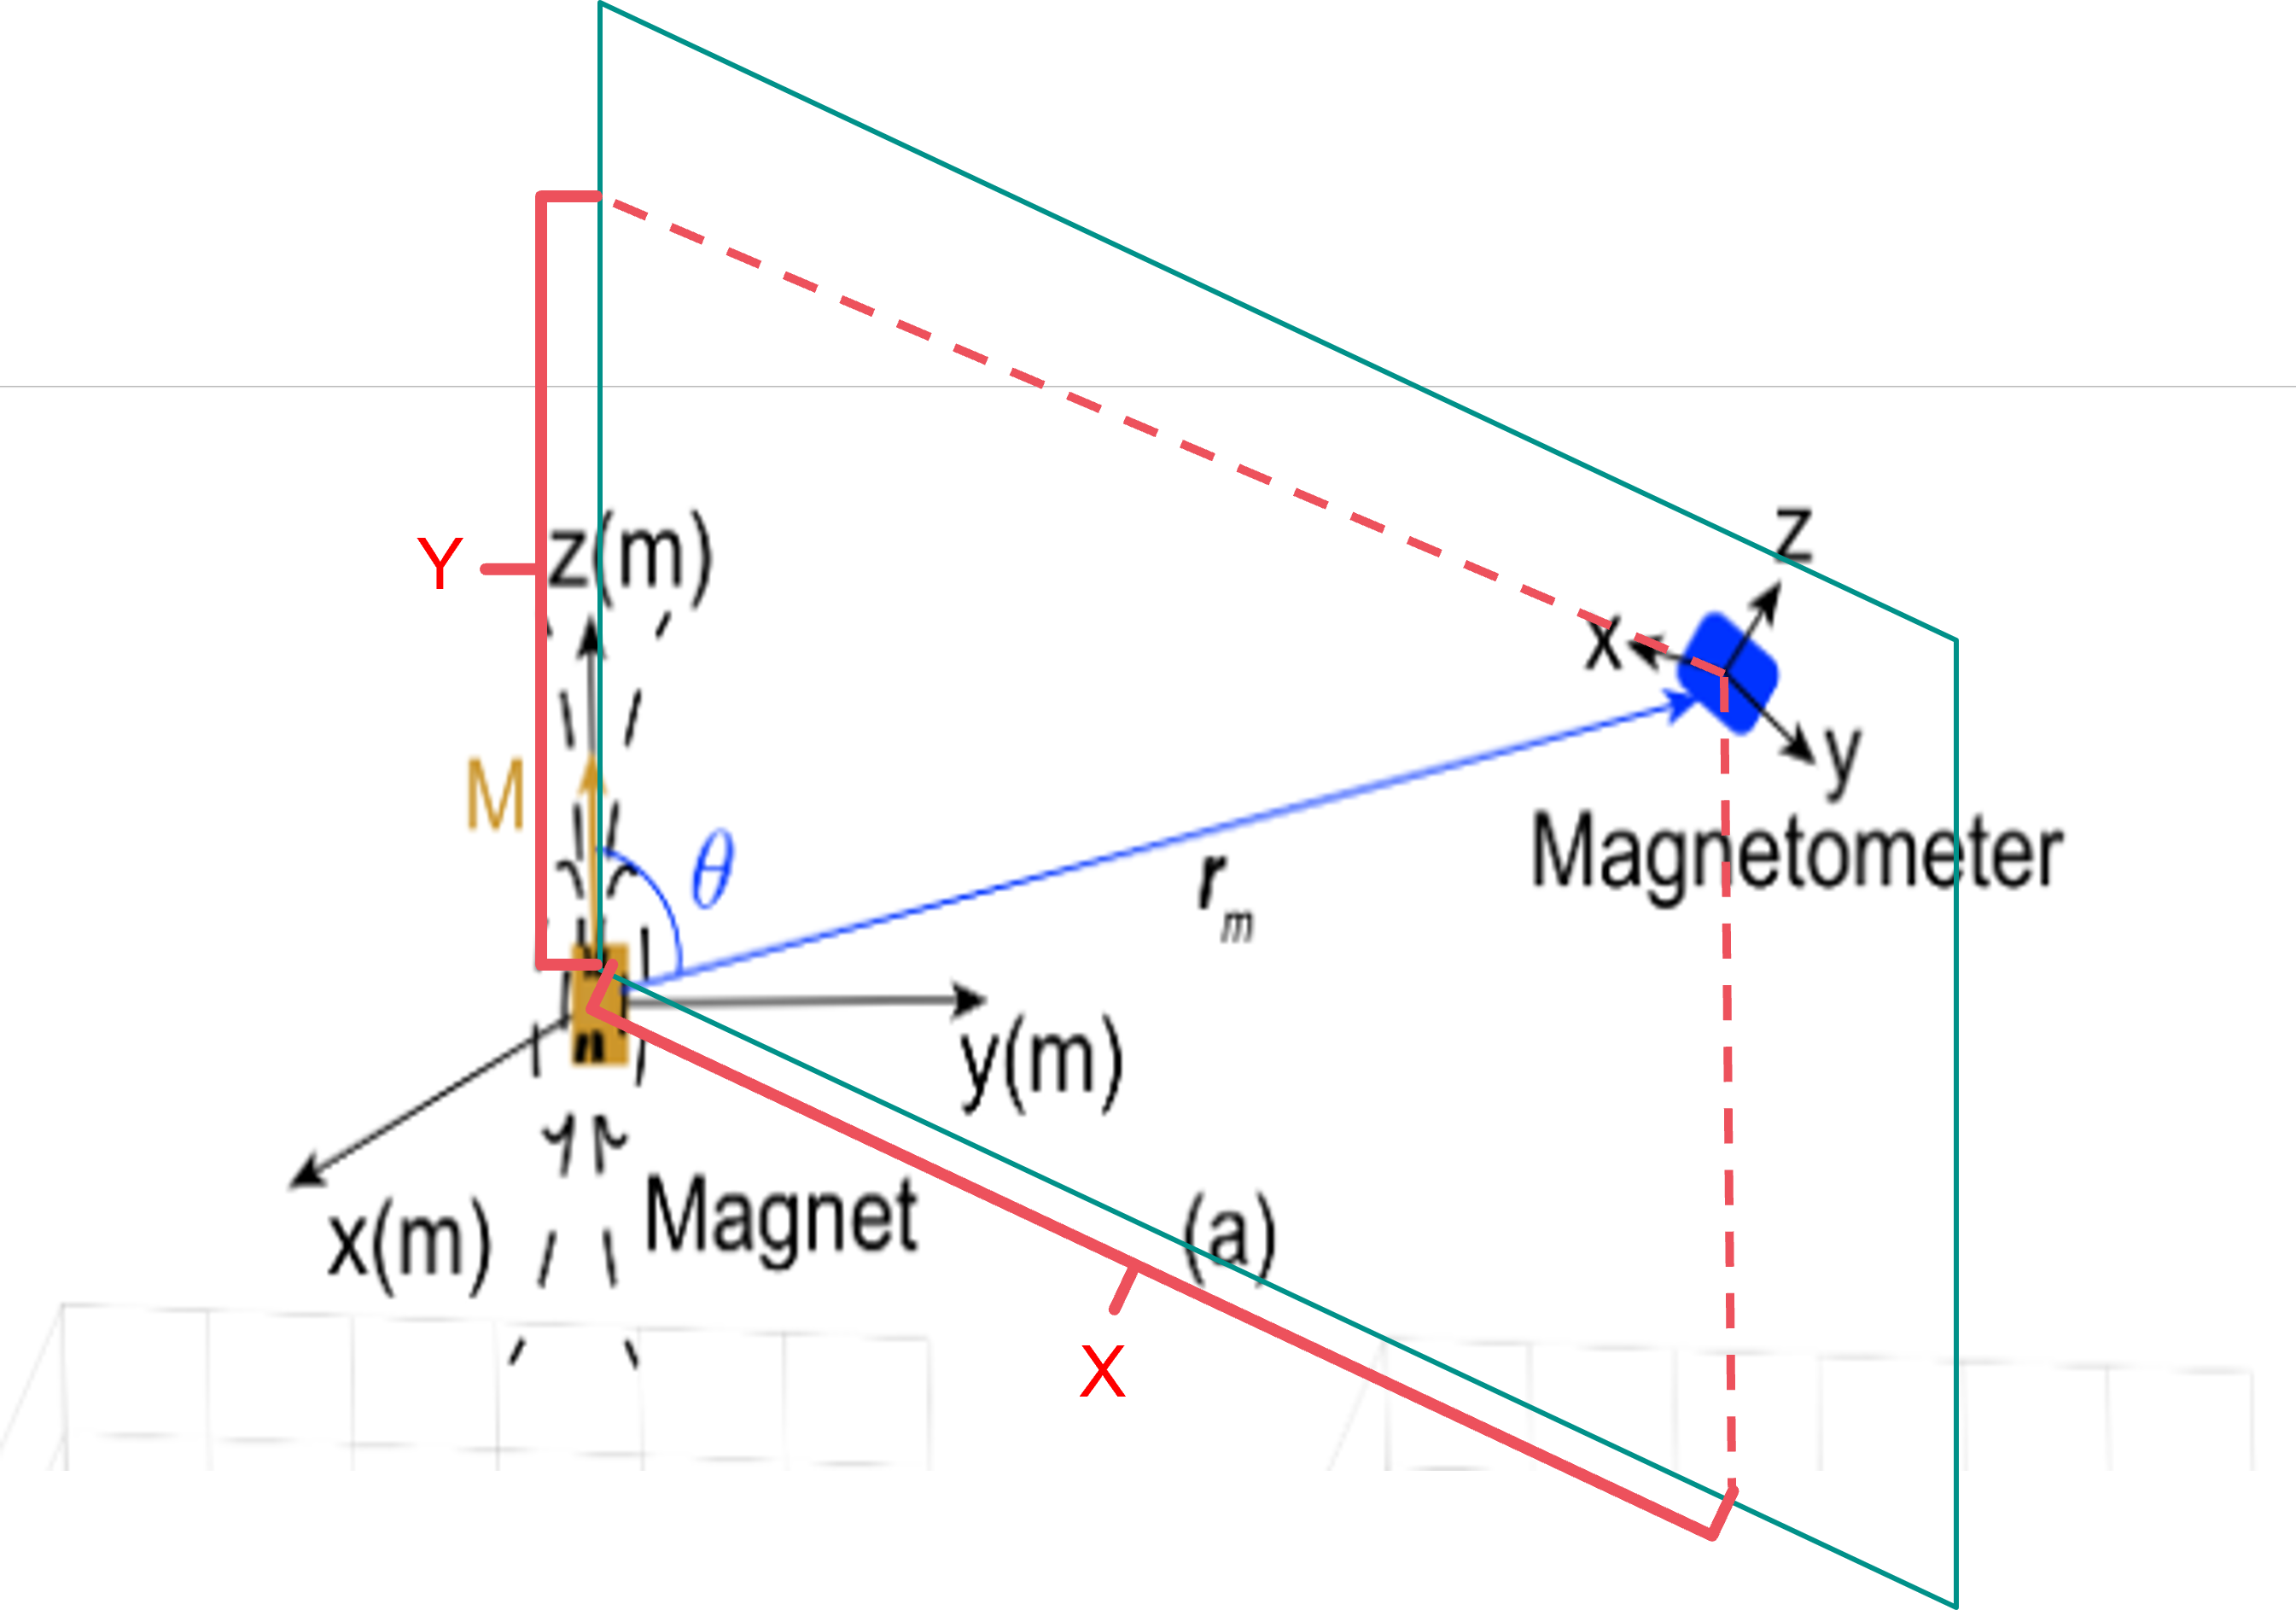
\includegraphics[width=0.8\linewidth]{gesture/solved-r-theta-diagram.png}
    \caption{\label{fig:solved-r-theta-diagram}Calculated Relative Position under Coordinate System}
\end{figure}

以动态追踪两个传感器为例,其在一定时间内累积的定位轨迹图如\autoref{fig:two-sensors-tracking}所示。其中,横坐标代表$r_m \times \sin{\theta}$,纵坐标代表$r_m \times \cos{\theta}$,单位均为cm

\begin{figure}[H]
    \centering
    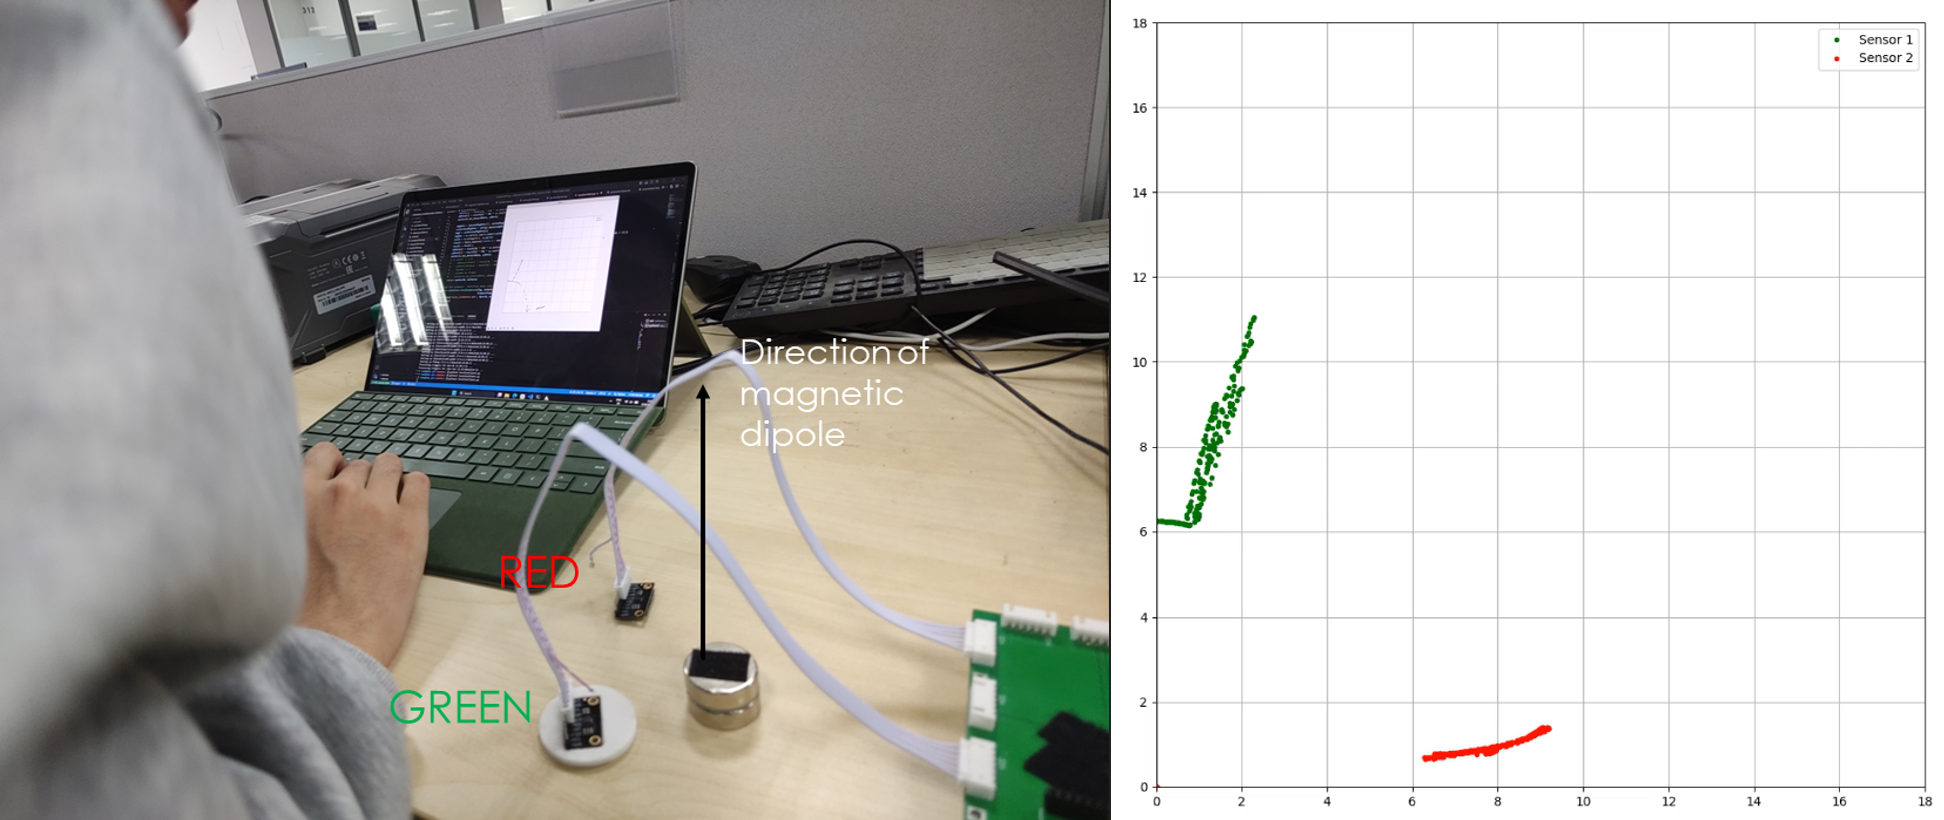
\includegraphics[width=\linewidth]{gesture/two-sensors-tracking.png}
    \caption{\label{fig:two-sensors-tracking}Dynamic Tracking of Two Sensors}
\end{figure}


\subsection{使用深度学习进行实时手势识别}
本毕设项目的其中一个可选目标是实现对多种手势的实时识别。
前几章所做的主要工作及后续的实时手势识别流程如\autoref{fig:repeat-subsequent-program-structure}所示

\begin{figure}[H]
    \centering
    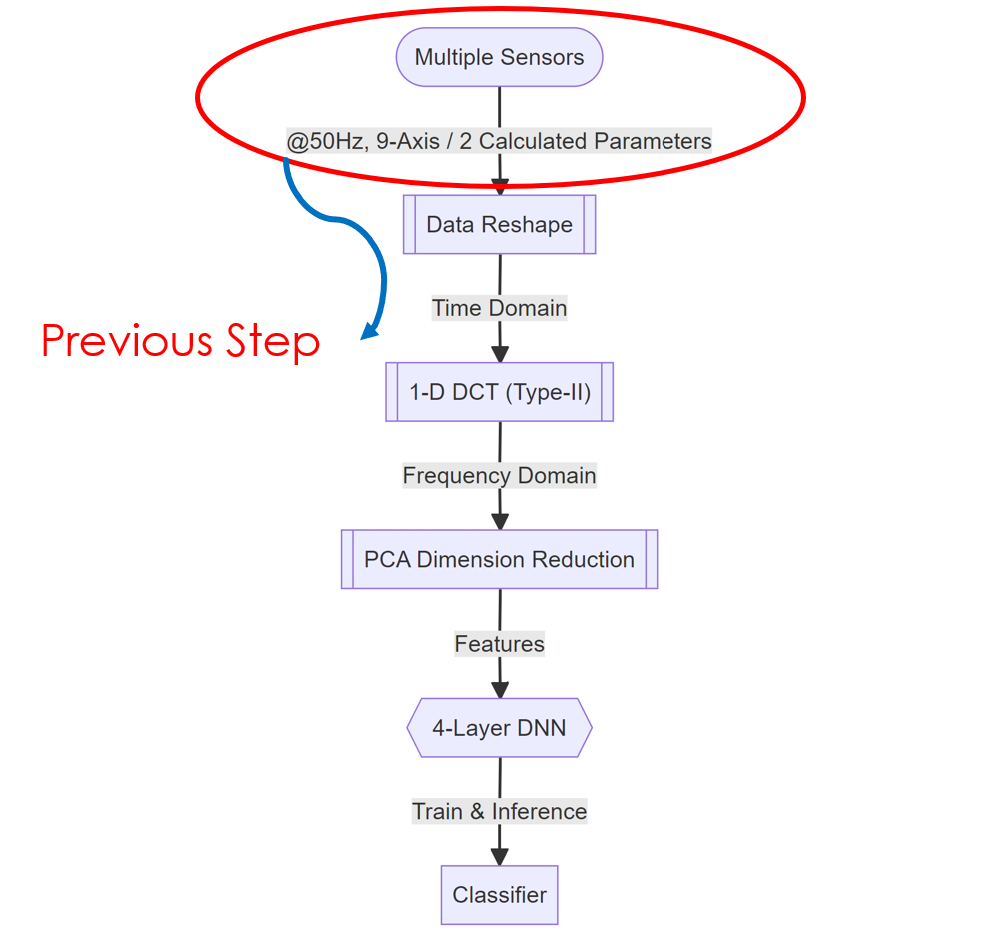
\includegraphics[width=0.5\linewidth]{software/subsequent-program-structure.png}
    \caption{\label{fig:repeat-subsequent-program-structure}Subsequent Dynamic Tracking and Gesture Recognition}
\end{figure}

在本毕设项目中,实时手势识别过程中的第一步是使用Raspberry Pi和I2C总线从实验手套读取传感器数据。传感器数据包括每个位于指尖的传感器相对于手背的相对位置信息。然后对这些数据进行处理和分析,以进行实时手势识别工作。

本节的主要工作及结果强依赖于本毕业设计项目中前几章的成果,是基于整个自底向上构建的智能手指运动追踪系统的综合实际应用
总体而言,本节展示了在此毕设项目上努力而取得的综合成果,突出了智能手指运动追踪系统在实时手势识别应用中的实用性和有效性。

\subsubsection{数据采集与记录}
如前所述,得益于整体系统的高性能与稳定实现,在戴上本项目中特制的手套后(见\autoref{fig:entire-device-front}),5个分别位于不同手指指尖上的传感器相对于手背的相对位置数据能够以超过50Hz的频率被实时更新与读取。
为此,我以Emoji表情包中的手势作为参考,从中选取了15个较为典型的手势作为实时手势识别的目标。这些手势如\autoref{fig:emoji-full-gesture}所示:

\begin{figure}[H]
    \centering
    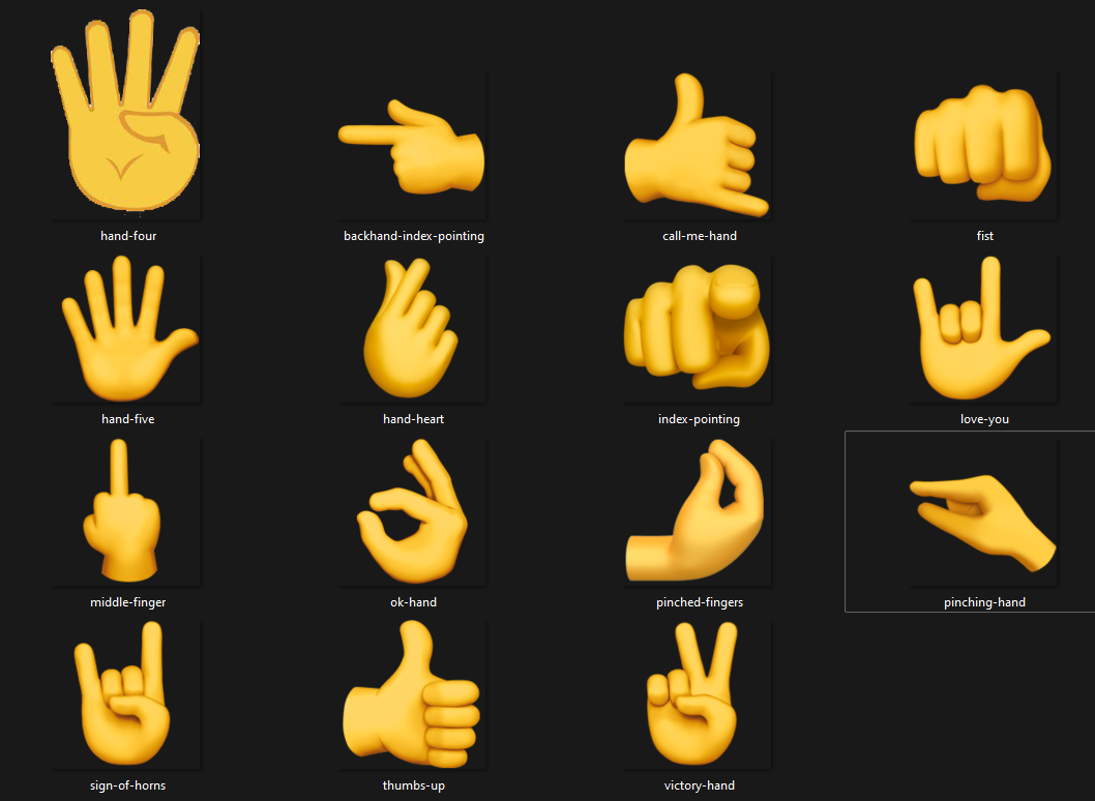
\includegraphics[width=.6\linewidth]{gesture/emoji-full-gesture.png}
    \caption{\label{fig:emoji-full-gesture}15 Reference Emoji Gestures}
\end{figure}

随后,戴上手套,分别作出相应的15个手势(参照选定的15种Emoji手势),并使用Python程序以固定50Hz的频率同时采集5个位于指尖的传感器的相对位置并记录。
在采集手势数据时(如\autoref{fig:collect-gesture-data}所示),为了保证所采集到的数据的通用性与泛化性,需要让手套在各个方向上进行运动变换(平移、旋转)。每个手势的数据采集时间控制在2分钟。

\begin{figure}[H]
    \centering
    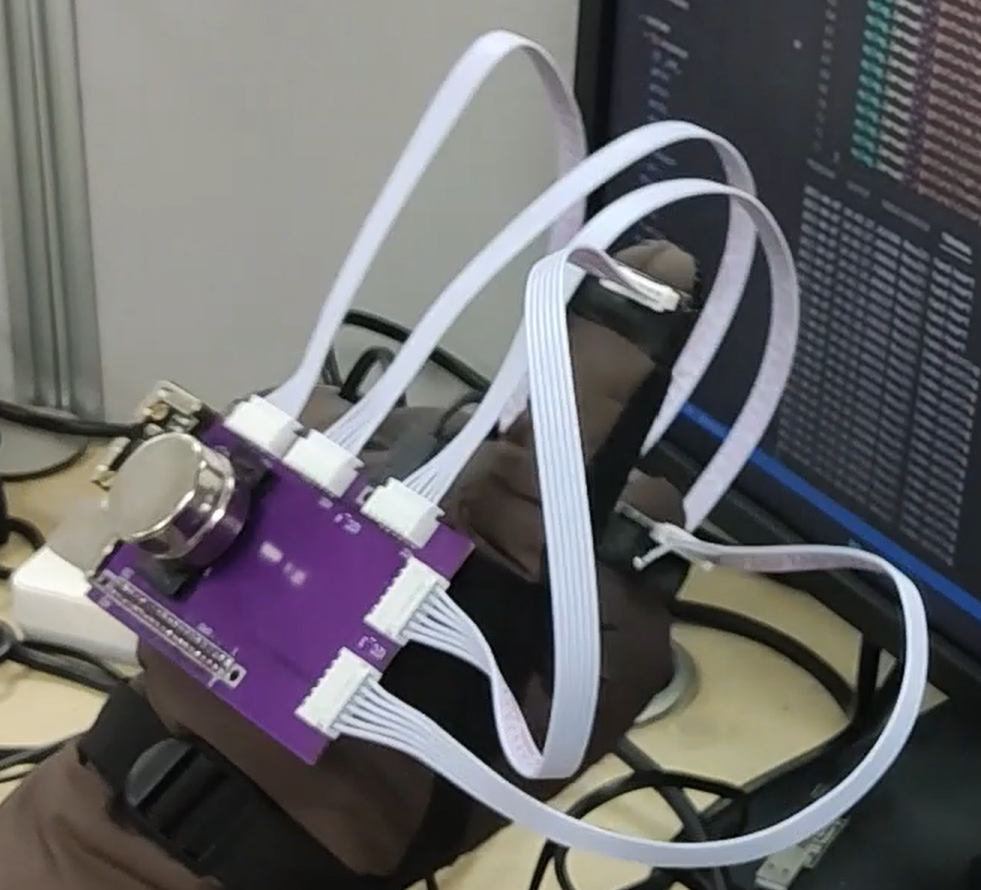
\includegraphics[width=.5\linewidth]{gesture/collect-gesture-data.png}
    \caption{\label{fig:collect-gesture-data}Collect Gesture Data}
\end{figure}

最终采集到的手势数据以二进制Numpy Array的格式进行保存(如\autoref{fig:gesture-numpy-array}所示):

\begin{figure}[H]
    \centering
    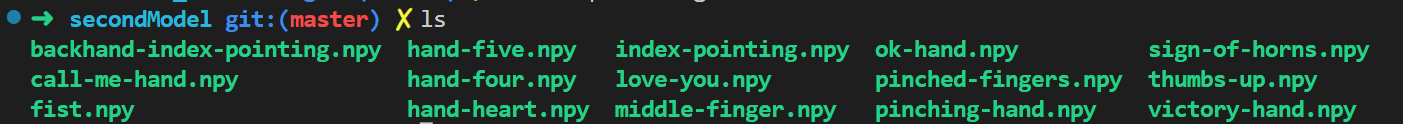
\includegraphics[width=.8\linewidth]{gesture/binary-gesture-data.png}
    \caption{\label{fig:binary-gesture-data}Saved Gesture Data}
\end{figure}

\subsubsection{数据预处理与数据集构建}
在正式训练前,需要先对采集到的数据进行预处理并构建相应的训练数据集与测试数据集。在本毕设项目中,训练集与测试集的比例为8:2:
\begin{enumerate}
    \item {\bfseries 数据分帧}:考虑到手指与手的运动,为了减小最终识别结果的波动率,提高识别结果的准确度,在数据预处理的过程中取每25个采样点为一个时间片(0.5秒),采用overlap的方式对原始数据集进行分帧。后续的手势识别流程均基于时间片进行
    \item {\bfseries DCT}:为了更好的捕捉手势识别时手指与手的动态信息与特征,对上一步中切分完毕的时间片做1维DCT(Type-II),从而将原始的时域数据映射到频域(如\autoref{fig:partial-data-after-dct}所示)
    \item {\bfseries PCA降维}:PCA是一种常用的数据降维技术,它可以将高维数据集转换为低维空间数据集,同时保留原始数据集的最重要的信息。但由于本项目中数据集的特征维度本就不大(50维),故最终并没有使用PCA降维。尽管如此,考虑到后续可能会使用具有更高维度特征,保留更多信息量的数据采集方法,此步骤应在整体流程中进行保留。
    \item {\bfseries 归一化}:对前几步处理完的数据在每一个特征维度上进行归一化,以确保训练过程中模型的收敛与稳定。
    \item {\bfseries 数据集与测试集划分}:随机抽取80\%的数据作为训练集,20\%的数据作为测试集,并使用Pytorch提供的API构建训练过程中使用的Dataset与Dataloader
\end{enumerate}

\begin{figure}[H]
    \centering
    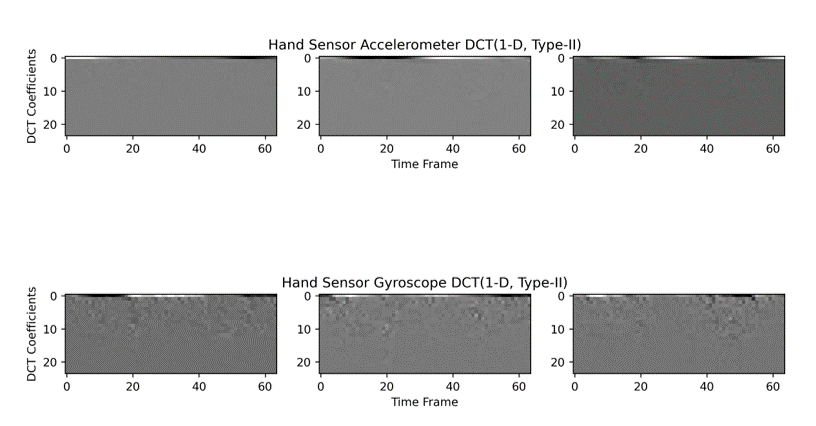
\includegraphics[width=.8\linewidth]{gesture/partial-data-after-dct.png}
    \caption{\label{fig:partial-data-after-dct}Data After 1D-DCT (Type-II, Partial)}
\end{figure}

\subsubsection{实时手势识别}
使用Pytorch构建一个简单的神经网络并使用前几节中构建的数据集进行训练,以最终执行实时手势识别任务(15分类)。由于数据的特征较为明显,故即使使用非常简单的全连接神经网络执行分类任务,其在训练集与测试集上的准确度也非常可观(如\autoref{fig:training-result}所示)。
同时,考虑到此模型将会被部署在树莓派4B平台上(算力资源有限),为保证手势识别结果的实时性,最终模型的规模和计算量不应过大。故权衡之下,本毕设项目中没有使用更高级、更复杂的模型来进一步提升识别准确度。

\begin{figure}[H]
    \centering
    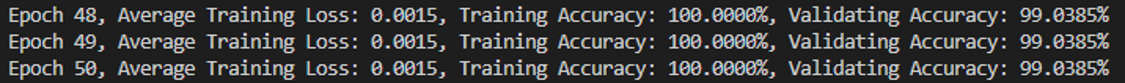
\includegraphics[width=.8\linewidth]{gesture/training-result.png}
    \caption{\label{fig:training-result}Training Result}
\end{figure}

最终,本毕设项目中的实时手势识别能够达到如下性能指标:
\begin{itemize}
    \item 50Hz+ sample frequency (6 sensors simultaneously)
    \item 2Hz+ recognition frequency
    \item Dynamic identification is possible
    \item Nearly 100\% Accuracy on Training Dataset
    \item 99\%+ Accuracy on Validating Dataset
\end{itemize}

识别效果(以其中两个手势为例)如\autoref{fig:recognition-result0}和\autoref{fig:recognition-result1}所示

\begin{figure}[H]
    \centering
    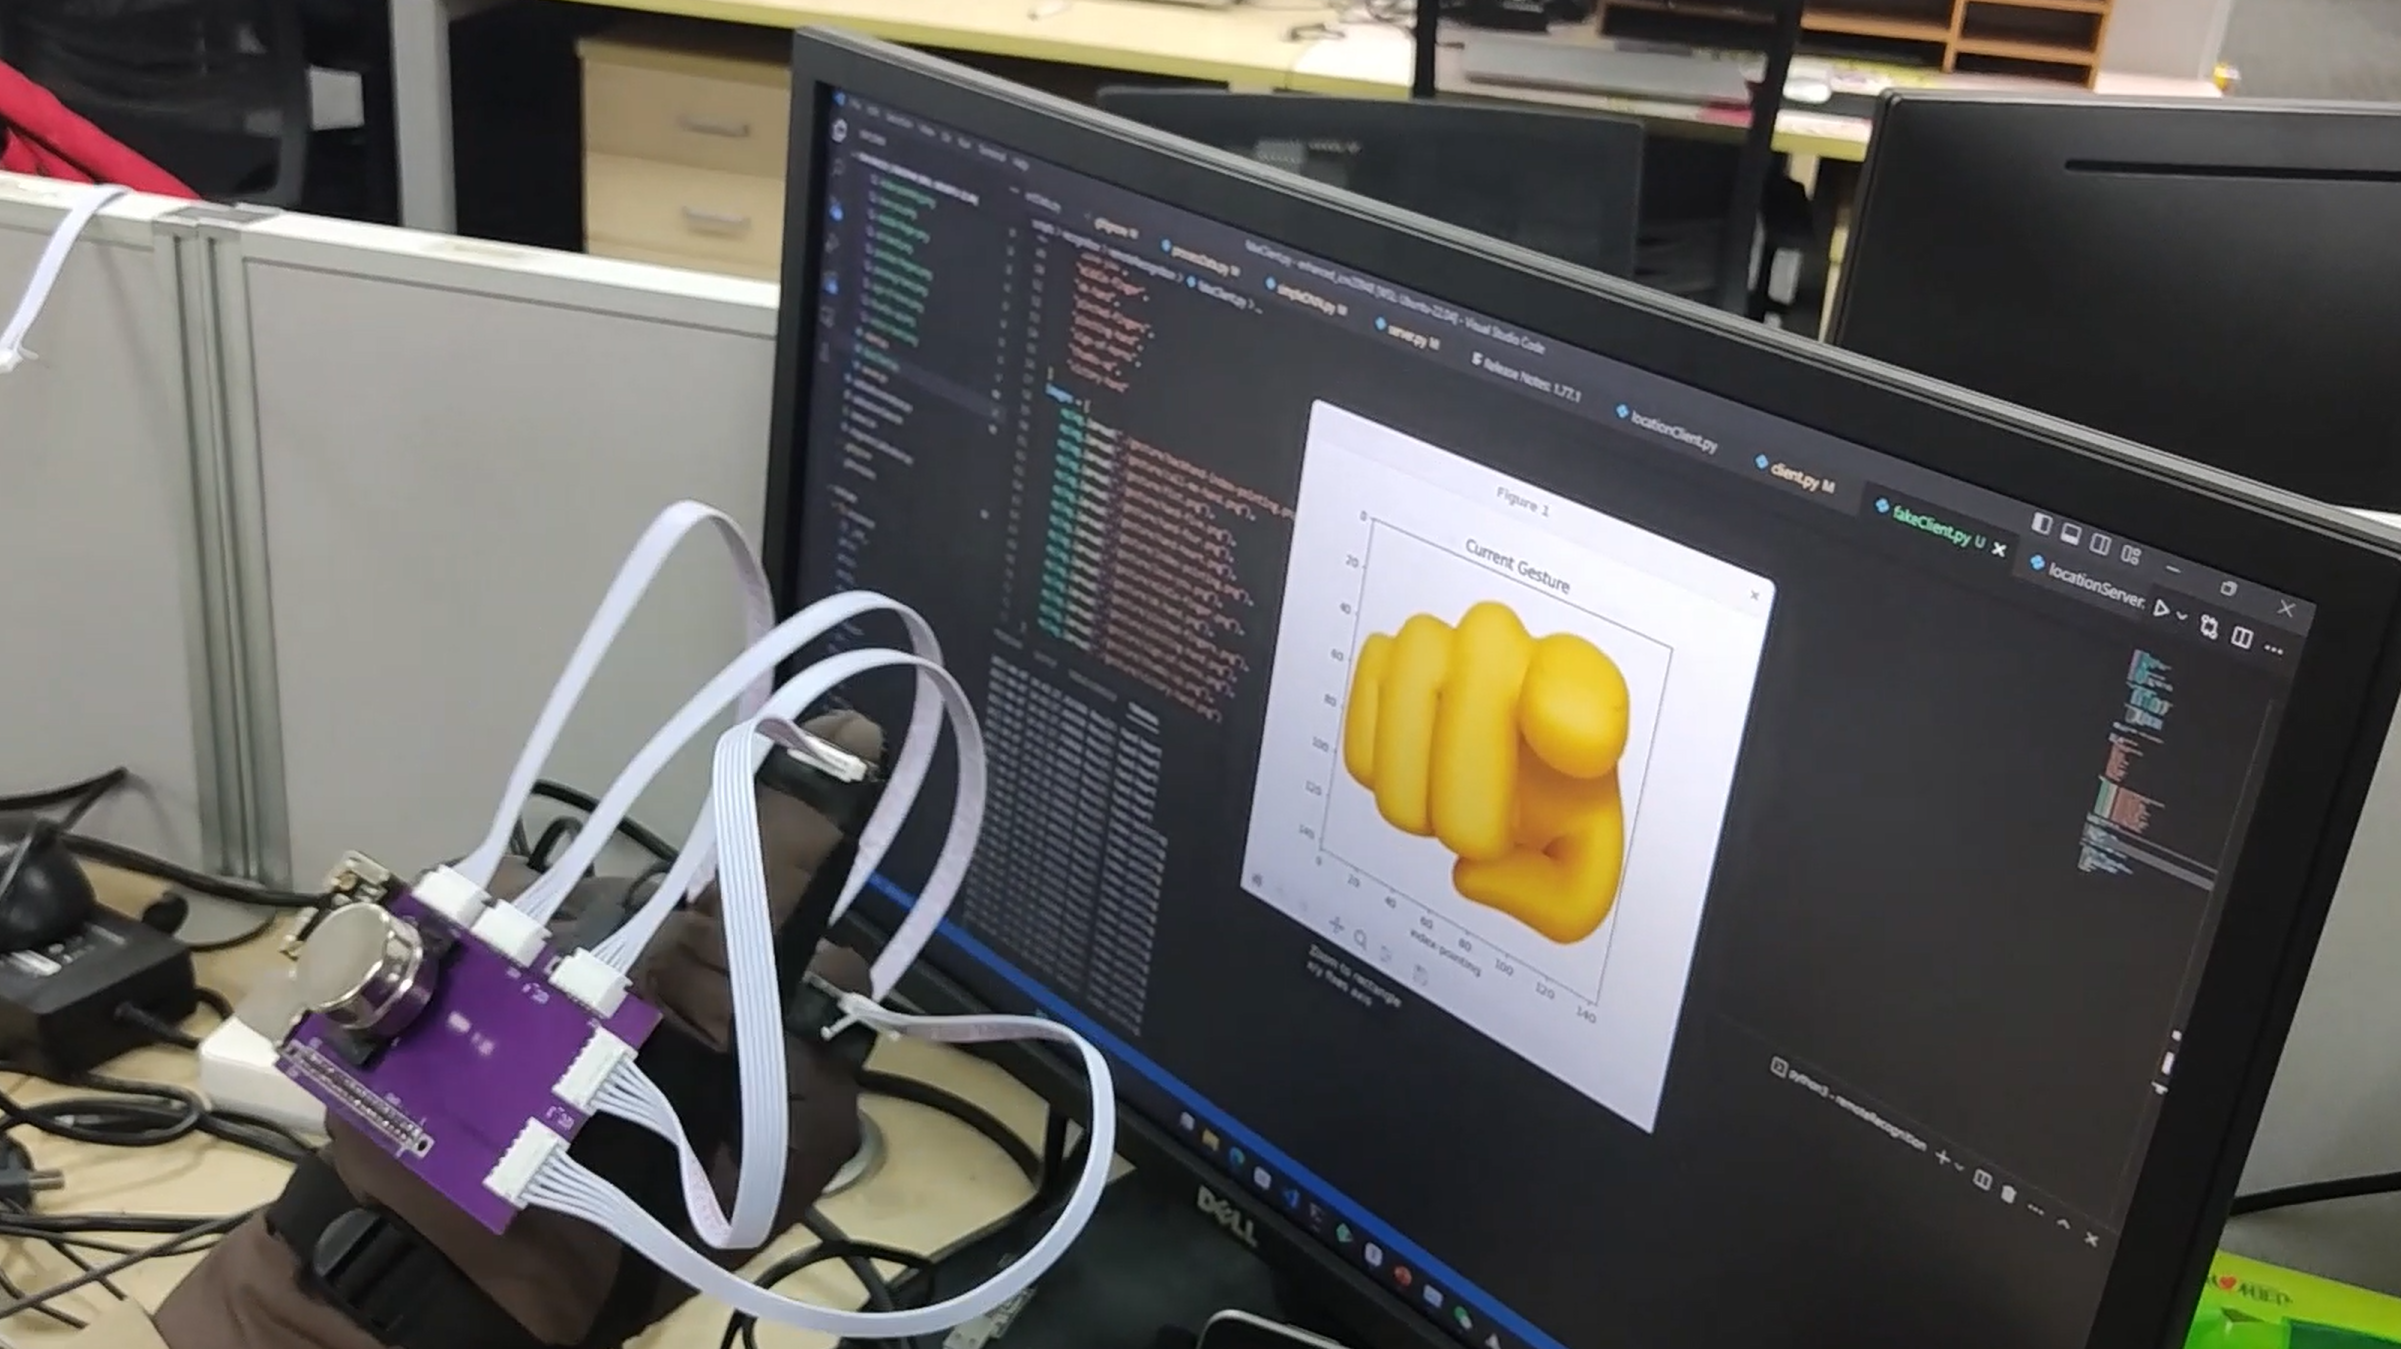
\includegraphics[width=.6\linewidth]{gesture/recognition-result0.png}
    \caption{\label{fig:recognition-result0}Real-Time Gesture Recognition Result (Index Pointing)}
\end{figure}

\begin{figure}[H]
    \centering
    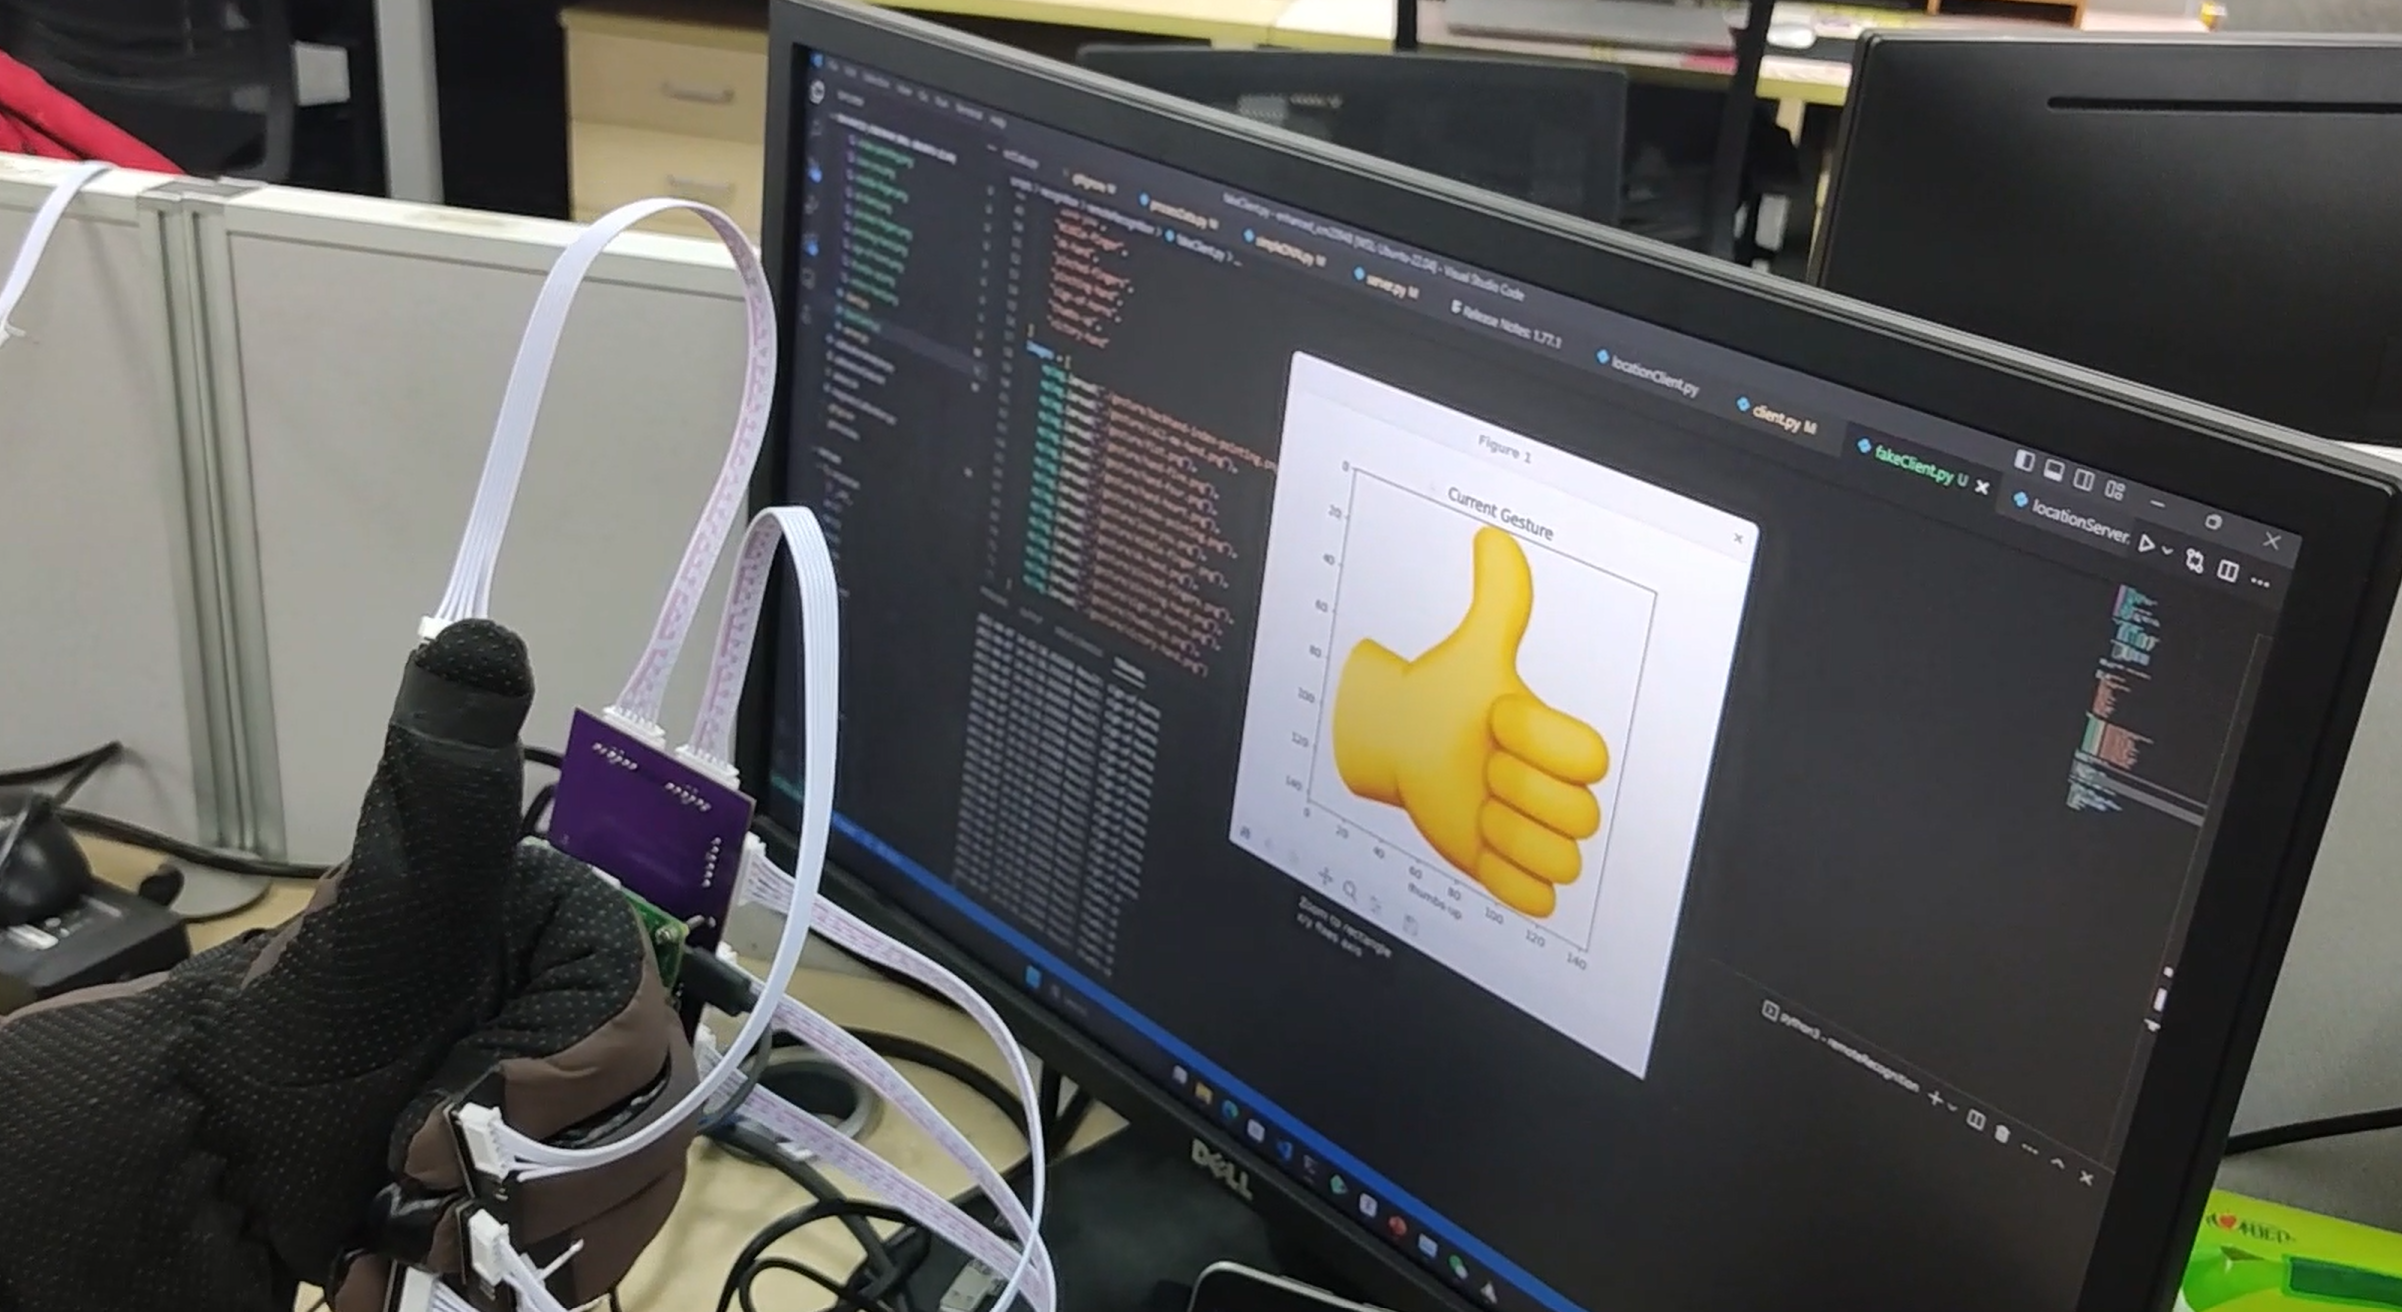
\includegraphics[width=.6\linewidth]{gesture/recognition-result1.png}
    \caption{\label{fig:recognition-result1}Real-Time Gesture Recognition Result (Thumbs Up)}
\end{figure}

\cleardoublepage
\section{总结}
总体而言,本毕设项目所做的工作可以被分为4个关键的部分:
\begin{enumerate}
    \item 开发一个使用C++后端的Python库,支持同时从多个ICM20948传感器高速读取数据(200Hz+)(并发布在GitHub和PyPI上)。
    \item 根据毕设项目的实际需求自行设计并打印了PCB电路板,以提高整体硬件系统的稳定性和集成度。
    \item 应用扩展卡尔曼滤波(EKF)算法和磁偶极子模型,动态地追踪和定位多个传感器的位置。
    \item 应用深度学习技术,支持对各种自定义手势的实时识别。
\end{enumerate}

综合起来,本毕设项目开发了一种利用多个磁传感器和惯性传感器的,低成本、高灵敏度、紧凑的智能手指运动追踪系统,并同时具有实时手势识别功能。此外,深度学习技术也被积极探索和应用,以提高实时手势识别的准确性。
此毕设项目中多传感器配置和深度学习技术的结合,为提供具有较好的灵敏度、较高的准确性和较强的经济性的多功能手指运动追踪系统做出了贡献。该系统在虚拟现实、增强现实、人机交互和生物医学工程等各个领域都有潜在的应用前景。